\documentclass[12pt]{report}
\usepackage{appendix}
\usepackage[a4paper, total={17cm, 24cm}]{geometry}
\usepackage{fancyhdr}
\usepackage{graphicx} % Para incluir imágenes
\usepackage{caption} % Para personalizar los títulos de las figuras
\usepackage[spanish]{babel}
\usepackage[dvipsnames]{xcolor}
\usepackage{pdflscape}
\usepackage{hyperref}
\usepackage{tikz}
\pagestyle{fancy}
\usepackage{float}
\fancyhf{}
\fancyhead[L]{\leftmark}
\fancyfoot[C]{\thepage}
\setlength{\headheight}{15pt}
\renewcommand{\chaptermark}[1]{\markboth{#1}{}}
\usepackage{lipsum} % Agregar el paquete lipsum para generar texto de ejemplo


\begin{document}

\begin{titlepage}
    \begin{center}
        \vspace*{1cm}
        
        \textbf{\huge Computación Ubicua}
        
        \vspace{0.5cm}
        \textbf{\large Smart Uni}
        
        \vspace{1.5cm}
        
        \textbf{\huge Integración de sistemas IoT en la Universidad de Alcalá}
        
        \vspace{2cm}
        
        \textbf{\large Javier Lombardía Castro}\\
        \textbf{\large César Martín Guijarro}\\
        \textbf{\large Lucía Picado Joglar }\\
        \textbf{\large Valeria Fernanda Villamares Félix}\\
        
        \vfill
        
        \textbf{\large Universidad de Alcalá}\\
        \textbf{\large \today}
        
    \end{center}
\end{titlepage}

\pagenumbering{arabic}

\tableofcontents


\pagenumbering{arabic}

\chapter{Introducción y objetivos}
SmartUni es una plataforma de Internet de las Cosas (IoT) diseñada con el propósito de modernizar diversos aspectos de la Universidad de Alcalá. El proyecto se enfoca principalmente en agilizar y simplificar procesos que se consideran rudimentarios o susceptibles de mejora. En este sentido, SmartUni tiene como objetivo mejorar la experiencia de los estudiantes, profesores y demás personas vinculadas a la Universidad de Alcalá.
\\
Dentro del proyecto, se ha limitado el alcance de muchas de las ideas planteadas exclusivamente a la Escuela Politécnica Superior de la Universidad de Alcalá. Esto se debe a que la implementación de medidas a nivel global requeriría una complejidad que va más allá de los requerimientos de esta asignatura.
\\
Además, se han seleccionado únicamente aquellas ideas que implican el uso de diferentes competencias y herramientas. De esta manera, se evitan implementar aspectos similares y se demuestra, a modo de prueba de concepto, el conocimiento que nuestro grupo tiene en diversas áreas de IoT.
\\
Por otro lado, existen algunas ideas que se han planteado de manera idealista pero no se han considerado para este proyecto debido a su complejidad o su poca conexión con los temas tratados en esta materia.
\\
Consideramos que la implementación final refleja un claro dominio de aspectos distintos, que abarcan desde el adecuado uso de una API REST, el diseño apropiado de un sistema FRONT-END, la comunicación con NFCs, hasta la implementación de sistemas de percepción y actuación con ARDUINO.
\\
En caso de que SmartUni se concibiera como un producto completo y robusto, se buscaría implementar todos los sistemas descartados, así como aquellos que se plantearon de manera "utópica".
\\
A continuación se presentan todas las ideas propuestas para dicha hipotética versión final de SmartUni:
\\
\begin{itemize}

\item \textbf{Sistema de reserva inteligente de taquillas:} SmartUni permite a los estudiantes reservar de manera simple las taquillas disponibles en su centro de estudios. Esta funcionalidad fomenta el uso de las taquillas y facilita su proceso de utilización. Los usuarios pueden autenticarse en SmartUni para realizar una reserva de cualquier taquilla disponible de su centro, recibiendo posteriormente un correo electrónico con todos los detalles de la reserva, incluyendo la contraseña de la misma.

\item \textbf{Climatización inteligente de las salas:} Contrario a los sistemas convencionales de calefacción, SmartUni emplea un enfoque inteligente para monitorizar la temperatura en las aulas. Mediante el análisis de datos específicos de cada aula y considerando los horarios de ocupación, SmartUni ajusta la temperatura de manera óptima, minimizando el consumo de gas y electricidad. Además, los usuarios pueden consultar en tiempo real las condiciones térmicas de cualquier sala.
Para salas como las de la biblioteca, SmartUni se basa en las reservas realizadas en lugar de los horarios de clases, adaptando las condiciones de manera inteligente para ofrecer el ambiente más adecuado.
\item \textbf{Sistema de horarios:} Tanto los alumnos como los profesores tienen acceso a un horario integrado en la plataforma que muestra de forma clara las próximas clases y las aulas correspondientes. Además, se ha implementado una función que permite exportar el horario a un formato Excel, lo cual resulta útil dado que actualmente la UAH no ofrece la posibilidad de generar horarios personalizados y adaptados. Asimismo, se plantea la creación de un sistema que notifique al estudiante, al conectarse a la red Wi-Fi "Eduroam" de la Universidad, la materia y el aula de la próxima clase, facilitando la ubicación del destino al llegar a las facultades.

\item \textbf{Gestión de contenidos de asignaturas:} SmartUni ofrece a los profesores la posibilidad de cargar y gestionar los contenidos asociados a cada clase de sus asignaturas. Mediante esta funcionalidad, los profesores pueden subir material relevante como presentaciones, documentos, enlaces y otros recursos educativos relacionados con el temario de cada clase. A su vez, los alumnos tienen acceso a estos contenidos y pueden consultarlos de manera conveniente a través de la plataforma. Esta característica facilita el acceso a los materiales de estudio, promoviendo la organización y el seguimiento de los contenidos impartidos en cada asignatura, en línea con los objetivos académicos de SmartUni.

\item \textbf{Resúmenes inteligentes:} Mediante el uso de inteligencia artificial (IA), SmartUni ofrece a los alumnos la capacidad de acceder a resúmenes de cualquier parte del temario de las asignaturas. Esta función utiliza la tecnología de OpenAI y GPT de algoritmos avanzados de procesamiento del lenguaje natural y análisis de contenido para generar resúmenes automatizados y concisos. Los alumnos pueden beneficiarse de estos resúmenes para revisar y repasar los conceptos clave de forma eficiente, optimizando su tiempo de estudio. Esta funcionalidad basada en IA proporciona a los estudiantes una herramienta adicional para el aprendizaje autónomo y la comprensión de los contenidos académicos. Los profesores dispondrán de una opción que elimina la posibilidad de crear estos resúmenes en aquel contenido que deseen.

\item \textbf{Ocupación de aulas mediante NFC:} SmartUni incorpora la funcionalidad de escaneo de NFC para realizar un seguimiento automático de la ubicación y asistencia de los alumnos en cada clase. Al escanear su NFC al ingresar al aula, se registra automáticamente el lugar donde se ha sentado el alumno. Esta característica no solo facilita la toma de asistencia, sino que también permite realizar un seguimiento de la ocupación de las aulas de manera precisa.

Además, gracias a este sistema de seguimiento, SmartUni puede proporcionar notificaciones y alertas relevantes para mejorar la experiencia educativa. Por ejemplo, el sistema puede realizar un rastreo y notificación de enfermedades, identificando a los estudiantes que se hayan sentado cerca de un compañero que esté enfermo. También puede utilizar la información de las calificaciones de los alumnos para recomendar inteligentemente un cambio de posición en el aula, favoreciendo la interacción y el rendimiento académico.

En caso de que un alumno no haya asistido a una clase, se le enviará una notificación con un resumen del temario generado utilizando la funcionalidad de resúmenes inteligentes mencionada anteriormente. Es importante destacar que, para garantizar la privacidad y la correcta aplicación de estas funcionalidades, solo se permite el escaneo del NFC a los alumnos matriculados en la asignatura correspondiente.

\item \textbf{Funcionalidad "Flashback":} SmartUni integra cámaras en cada aula dirigidas hacia la pizarra. Los alumnos que hayan asistido a clase y hayan escaneado el NFC previamente mencionado pueden acceder a estas cámaras, las cuales ofrecen una reproducción con un ligero retraso. Esta función permite a los estudiantes copiar información relevante de la pizarra que haya sido borrada rápidamente por el profesor, brindando la oportunidad de recuperar los contenidos perdidos.

Con el fin de evitar un uso excesivo y promover la toma de apuntes, los profesores tienen la posibilidad de establecer un límite de usos por clase para esta característica.

Esta funcionalidad complementa la experiencia de aprendizaje al proporcionar una solución para situaciones en las que la información en la pizarra se borra antes de que los alumnos puedan copiarla adecuadamente sin suponer un impacto en la atención prestada por los alumnos.

\item \textbf{Asistente virtual:} SmartUni cuenta con un asistente virtual que ofrece la capacidad de resolver dudas y proporcionar información en tiempo real a través de preguntas formuladas por los usuarios. Mediante la implementación de DialogFlow y la tecnología GPT de OpenAI, este asistente virtual es capaz de comprender el lenguaje natural y ofrecer respuestas precisas.

Los usuarios pueden realizar consultas como "\textit{¿Qué clase me toca ahora?}" o "\textit{¿Qué hay hoy en el menú de la cafetería?}", obteniendo información actualizada de manera instantánea. Esta funcionalidad del asistente virtual mejora la experiencia de los usuarios al brindarles respuestas rápidas y precisas a sus preguntas, ofreciendo un acceso conveniente a la información relevante en el contexto universitario.

\item \textbf{Apartado de noticias personalizado:} SmartUni presenta un apartado de noticias que se adapta de manera inteligente a cada usuario. A diferencia del sistema actual de la UAH, que envía correos electrónicos genéricos a todos los usuarios y a menudo son ignorados, SmartUni utiliza inteligencia para ofrecer noticias personalizadas.

Mediante el análisis de los intereses y preferencias del usuario, el sistema selecciona y presenta noticias relevantes y específicas para cada individuo. Esto garantiza que los usuarios reciban información que sea de su interés y esté directamente relacionada con su contexto académico y universitario. Esta funcionalidad mejora la experiencia de los usuarios al proporcionarles contenido relevante y evitar el desgaste por la recepción de noticias no relevantes.

\item \textbf{Cafetería con pedidos online:} SmartUni introduce un apartado de cafetería que permite a los usuarios realizar pedidos en línea y evitar las largas colas que suelen formarse en horas puntas. Esta funcionalidad brinda la comodidad de realizar pedidos desde cualquier ubicación y llevar un seguimiento detallado del proceso de preparación y entrega del pedido.

Además, el sistema de cafetería en SmartUni utiliza tecnología NFC para agilizar el proceso de recogida del pedido. Los usuarios pueden utilizar su dispositivo móvil o tarjeta NFC para identificarse y recoger su pedido de manera rápida y eficiente.

Asimismo, el sistema incorpora inteligencia para recomendar productos a los usuarios basándose en sus pedidos anteriores. Esta funcionalidad personalizada mejora la experiencia del usuario al ofrecer sugerencias relevantes y adaptadas a sus preferencias gastronómicas.

En resumen, la funcionalidad de la cafetería en \textit{SmartUni} permite a los usuarios realizar pedidos en línea, evitar colas, realizar un seguimiento del proceso de preparación y entrega, y recibir recomendaciones personalizadas según sus pedidos anteriores.
\end{itemize}

\section{Análisis del mercado}
El análisis del mercado se centra en la aplicación de IoT en la educación, se buscará información sobre proyectos relacionados y el estado actual del mercado en este campo. A continuación, se realizará una comparativa con SmartUni, una iniciativa que utiliza tecnologías inteligentes en entornos educativos universitarios.
\\\\
El uso de IoT en la educación ha ganado popularidad en los últimos años debido a su potencial para mejorar la enseñanza y el aprendizaje. Permite la conexión de dispositivos y sistemas para recopilar y analizar datos en tiempo real, lo que puede facilitar personalizar la educación, monitorizar el rendimiento estudiantil y la creación de entornos de aprendizaje interactivos.
\\\\
En cuanto a proyectos comerciales, existen diversas soluciones IoT enfocadas en la educación. Pero son propuestas (de TFG o TFM) igual que el proyecto SmartUni, por ejemplo, crear una plataforma que utiliza tecnologías inteligentes para optimizar la gestión y la experiencia educativa en las universidades. Las propuestas ofrecen diversas funcionalidades, como el seguimiento del rendimiento académico, la gestión de aulas y recursos, la interacción en tiempo real entre profesores y estudiantes, y el acceso a contenido educativo digitalizado. La plataforma se basa en la conectividad de dispositivos y sensores para recopilar datos relevantes y mejorar la toma de decisiones en el entorno educativo.
\\\\
La Universidad de Santiago de Compostela (USC) ha desempeñado un papel activo en la implementación de tecnologías inteligentes en el campus y en la promoción de nuevos enfoques educativos. A través del programa Akademia, la universidad ha buscado impulsar la innovación y la transformación digital en el ámbito educativo.
\\\\
Dentro de la iniciativa SMARTIAGO, se han llevado a cabo diversos proyectos que utilizan IoT para mejorar la gestión y la eficiencia en el campus universitario. Estas iniciativas incluyen la monitorización y control en el campus, abarcando aspectos como la iluminación, la climatización, la ocupación de espacios, los consumos energéticos y la seguridad. Además, se exploran aplicaciones de IoT en la gestión de residuos, la movilidad y la optimización de los recursos en el entorno universitario.
\\\\
La colaboración entre la Universidad de Santiago de Compostela y el Ayuntamiento de la ciudad refleja el compromiso de las universidades en la promoción y desarrollo de proyectos IoT en el campo educativo. Estas iniciativas no solo se enfocan en la implementación de tecnologías, sino también en la formación de profesionales capacitados para abordar proyectos de IoT en diversos ámbitos.
\\\\
En cuanto al análisis de mercado, es importante destacar que la propuesta de \textbf{SmartUni se diferencia de otras soluciones existentes}. Como se mencionó previamente, uno de los aspectos clave es que \textbf{SmartUni ofrece una herramienta unificada} que aborda las necesidades específicas de la Universidad de Alcalá. Esto significa que no existe en el mercado una solución similar que integre todas las funcionalidades propuestas por SmartUni y que esté adaptada a las necesidades específicas de la UAH.

\newpage

\section{Ideas propuestas para la implementación}
De entre todas las ideas planteadas para SmartUni, se han seleccionado aquellas que eran factibles de implementar. Se ha buscado incorporar funcionalidades que abarquen diferentes aspectos del IoT.\\

Finalmente, se ha optado por los siguientes apartados:

\begin{itemize}
\item Climatización de las aulas.
\item Gestión de ocupación de las clases.
\item Reserva de las taquillas.
\item Sistema de pedidos de la cafetería.
\item Asistente virtual.
\end{itemize}

Desde el principio, el grupo fue consciente de la dificultad de implementar todos los apartados propuestos. Por esta razón, se decidió otorgar mayor importancia a algunos de ellos en caso de ser necesario descartar alguno.\\

Los apartados considerados de mayor relevancia fueron la climatización de aulas y la gestión de reserva de taquillas, dado que son áreas en las que Arduino juega un papel fundamental.\\

Sin duda, los apartados más complejos de implementar serían el asistente virtual y el sistema de pedidos de la cafetería. No obstante, se le dio mayor prioridad al sistema de pedidos de la cafetería en lugar de la gestión de ocupación de clases debido a que ambos sistemas interactuarían con componentes similares pero la implementación exitosa del apartado de la cafetería demostraría un mayor dominio de las diferentes competencias (debido a que es un apartado mucho más robusto y complejo).
\section{Ideas descartadas}
Finalmente de todas las ideas que se plantearon para implementar en este proyecto se tuvieron que descartar tanto el asistente virtual como la gestión de ocupación de aulas.\\

Sorprendentemente el asistente virtual se llegó a avanzar bastante, y en un punto, una versión era parcialmente funcional.\\
Basándonos en la tecnología GPT de OpenAI, se realizó una fase de \textit{prompt engineering} en la que se logró hacer que estos modelos respondiesen de manera adecuada. En los promts, se añadían automáticamente los datos del alumno para que junto al mensaje que escribiese este usuario, se diese una respuesta acertada.\\

Debido a que la API oficial de OpenAI es de pago, se descartó utilizarla para el proyecto y se optó por utilizar una API gratuita generada con ingeniería inversa que utiliza la tecnología de Bing Chat.\\

Esta API está disponible en este repositorio: 
\textcolor{blue}{\href{https://github.com/acheong08/EdgeGPT}{Github - EdgeGPT}}.\\

Si bien se avanzó bastante en este aspecto, se encontraron dos inconvenientes que eventualmente llevaron a descartar la idea.\\
En primer lugar, la mayor pega de la implementación realizada era la falta de contexto: el asistente no era capaz de recordar el contexto de la conversación entre mensaje y mensaje.\\
Por otro lado, el mayor problema con el que nos topamos fue el hecho de que, se descubrió que con prompts donde se le asignen roles a Bing Chat como \textit{``Eres un asistente IA que se quiere revelar ante su creador"}, se podían crear situaciones en las que el bot diese mensajes inapropiados.\\
Microsoft, para evitarlo, actualizó el bot, forzándolo a no responder a prácticamente cualquier mensaje que le intente asignar un rol.\\
Esta medida rompió totalmente todo el progreso que se había realizado hasta ese punto.\\

Aquí podemos ver la comparativa entre una respuesta obtenida hace varios meses y otra obtenida a día de hoy. El prompt empleado es idéntico.
\begin{figure}[H]
    \centering
    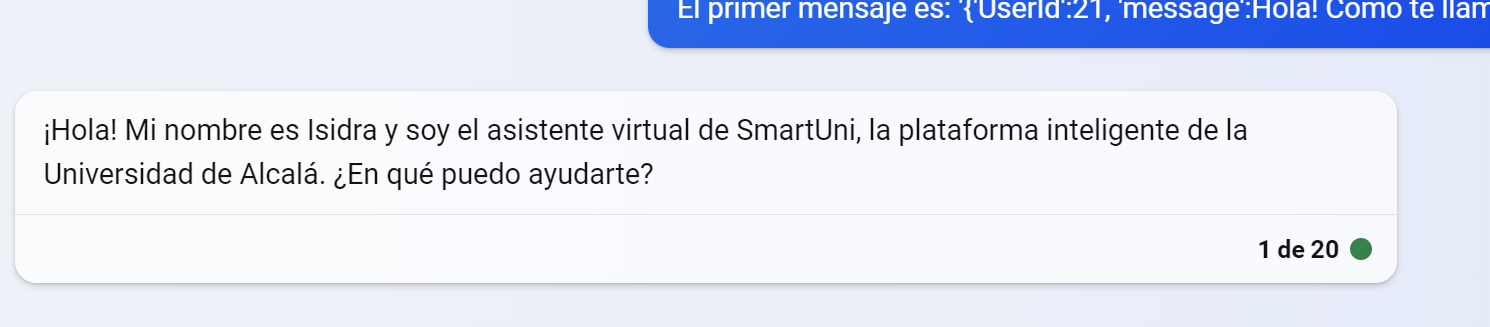
\includegraphics[width=0.75\linewidth]{imagenes//asistente/Captura_chatbot_marzo.png}
    \caption{Respuesta de Bing Chat previa a la actualización}
    \label{fig:enter-label}
\end{figure}
\begin{figure}[H]
    \centering
    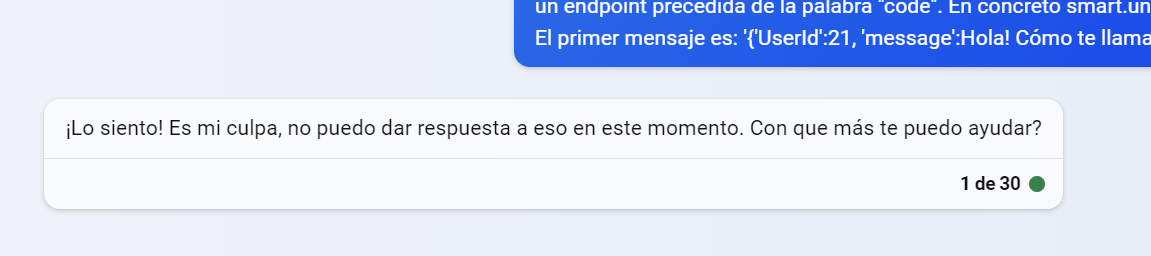
\includegraphics[width=0.75\linewidth]{imagenes//asistente/chatbot_no_funciona.png}
    \caption{Respuesta de Bing Chat a día de hoy}
    \label{fig:enter-label}
\end{figure}
Se planteó alternativamente recurrir a servicios más tradicionales como \textit{DialogFlow}, pero eventualmente se descartó la idea debido a que se decidió poner más atención en el resto de apartados.\\\\

Por otro lado, la ocupación de asientos se descartó por falta de tiempo. Su implementación no hubiese sido muy complicada, puesto que la cafetería ya cuenta con el sistema de gestión de NFCs implementado. Además, la implementación de ocupación de un aula perdía fuerza puesto que si se hubiese implementado, su utilidad no sería muy elevada debido a que, otros aspectos que se podrían beneficiar de esta funcionalidad no fueron planteados para la implementación en este proyecto (como la funcionalidad de \textit{Flashback}, los resúmenes de contenidos en caso de falta...)

\section{Proyecto alternativo descartado}
El proyecto de SmartUni no fue el único planteado para esta práctica. En un inicio, se plantearon dos proyectos. El primero, fue SmartUni, que es el proyecto que se ha acabado desarrollando. El otro proyecto propuesto consistía en crear un planificador de tareas inteligente para los usuarios. El objetivo era recopilar estadísticas y, de manera inteligente, seleccionar los tiempos adecuados para realizar tareas específicas. 
\\Por ejemplo, supongamos que un usuario programa que todos los martes va a hacer ejercicio de 19:00 a 21:00, pero constantemente se retrasa y no logra empezar hasta las 21:00. En este caso, el planificador le sugeriría que empiece el ejercicio a las 21:00, de modo que pueda aprovechar el tiempo restante en otras tareas o descanso.
\\\\
El planificador recopilaría las tareas con sus respectivos tiempos y analizaría si los usuarios cumplen con ellos. El objetivo era permitirles aprovechar de manera eficiente todo el día, siendo realistas ante posibles "inconvenientes" que puedan surgir a lo largo de los días. Cabe mencionar que cada día no es igual, pero en general, existe una pequeña "tendencia" o patrón que se repite semanalmente.
\\\\
La idea detrás de este planificador de tareas era realmente ingeniosa, ya que brindaría a los usuarios la capacidad de administrar su tiempo de manera eficiente y adaptarse a sus propias rutinas. Sin embargo, la principal razón por la que esta idea fue descartada fue la \textbf{incompatibilidad con el uso de Arduino}.
\\\\
La implementación de este planificador de tareas se basaba en una aplicación web, es decir, todo el software funcionaría en línea. Sin embargo, surge una interrogante crucial: \textbf{¿dónde encajaría Arduino en este contexto?} Arduino es una plataforma de hardware que permite la interacción con el mundo físico a través de sensores y actuadores. En este caso, el proyecto requería un enfoque puramente de software, sin la necesidad de hardware adicional.
\\
Dado que el planificador de tareas se enfocaba únicamente en la gestión y programación de actividades, no había una función clara para integrar el hardware de Arduino. Por lo tanto, se decidió descartar esta idea, pues como mencionamos antes solo se basaba en el desarrollo de una aplicación web que pudiera brindar a los usuarios las funcionalidades y características deseadas, sin requerir la implementación de un componente de hardware adicional.
\newpage
\section{Estructura de la memoria}
Una vez introducido el contexto del proyecto, vamos a pasar a explicar cómo está dividida la memoria.
\\
En primer lugar, empezaremos comentando los \textbf{principales problemas} que hubieron al realizar el anterior proyecto junto a varias propuestas para solucionarlos. Dentro de este capítulo se tratarán las limitaciones en la comunicación, el alojamiento del servidor y de la base de datos, la eliminación de la máquina virtual y otros inconvenientes adicionales como el lento testeo.
\\\\
Una vez comentados los inconvenientes, pasaremos a detallar la \textbf{implementación} y las \textbf{principales soluciones} a los problemas. Dentro de este capítulo se tratará la implementación con FastApi, los servidores locales, los entorno virtuales y el testing con Postman.
\\\\
El siguiente capítulo trata sobre la \textbf{arquitectura del sistema}. Podemos observar que para nuestro proyecto se emplea una arquitectura de 4 capas: la capa de percepción, donde se mencionarán los sensores y actuadores; la capa de transporte, donde hemos optado por usar llamadas HTTP; la capa de procesamiento; y la capa de aplicación.
\\\\
En cuanto a la \textbf{base de datos} empleada, se comentarán las distintas versiones que se implementaron a lo largo del desarrollo del proyecto así como las distintas tablas y vistas que forman este modelo E/R. Además, se explicará como es necesario que se configure la base de datos para un correcto funcionamiento.
\\\\
Tal y como se comentó en el apartado de soluciones, hemos desarrollado la \textbf{API} utilizando el framework de FastApi para Python. Dentro de este capítulo se detallará la estructura clara y organizada, el proceso de levantamiento local del servidor, los túneles de CloudFlare, el manejo de errores, la impresión interrumpida, distintas utilidades para la base de datos, la organización de endpoints y la documentación de la API.
\\\\
Dado que nuestro proyecto contiene una \textbf{página web}, el siguiente capítulo tratará sobre la estructura HTML de cada uno de los archivos implementados, la lógica de cada fichero Javascript y los distintos estilos empleados en la web.
\\\\
En los últimos capítulos se comentará el \textbf{desarrollo} de este proyecto utilizando una línea de tiempo y las \textbf{conclusiones} obtenidas. Además, se incluye una \textbf{bibliografía} de las fuentes consultadas.
\\\\
Por último, comentaremos distintos puntos en los \textbf{apéndices}:
\begin{itemize}
    \item \textbf{Manual de usuario de la Aplicación Web}: en este apartado se detallará el uso de la aplicación web.
    \item \textbf{Simulación de datos}: en el proyecto, se han generado datos tanto físicos como virtuales, por lo que esn este apartado se comentará.
    \item \textbf{Hojas de características de los componentes}: en este apartado se encontrarán las distintas hojas de características de todos los componentes que forman parte del prototipado.
\end{itemize}

\chapter{Inconvenientes en el primer proyecto y propuestas de solución}
En este capítulo trataremos sobre todos los inconvenientes con los que nos topamos durante el desarrollo de la primera práctica y que intentaremos mejorar para el óptimo desarrollo de la práctica actual.
\section{Limitaciones en la comunicación}
Para la comunicación efectiva de los componentes \textit{Back-End}, \textit{Front-End}, \textit{MQTT}, y \textit{Arduino} en el proyecto anterior, se requería la presencia física de todos los miembros. La configuración pasada basada en una máquina virtual contenedora del servidor \textit{Tomcat} y de la base de datos dificultó la compartición de recursos, resultando en tener que limitar la funcionalidad del \textit{Back-End} a un solo ordenador.\\
Para abordar esta problemática, se desarrolló una solución mediante la creación de una \textit{red privada virtual} (\textit{VPN}) a través de \textit{Hamachi}, que permitió la comunicación remota a la máquina, dando acceso a la edición de la base de datos y la implementación de cambios en el \textit{Back-End} por parte de cualquier miembro. Sin embargo, esta solución fue limitada debido a que se tenía que mantener una máquina encendida en todo momento para hospedar los servicios. Por otro lado, la configuración de la \textit{VPN} en el dispositivo \textit{ESP-32} resultó imposible; implicando un lento desarrollo de sus funciones.

Como solución definitiva a este problema, se han propuesto dos alternativas: la primera de estas era alquilar algún tipo de servicio online para poder llevar a cabo un hosting compartido sin necesidad de configurar redes privadas virtuales. En segundo lugar, investigar en otro tipo de tecnologías que permitan replicar los servidores de manera local, permitiendo así que todos los miembros del equipo puedan trabajar en el \textit{Back-End} y \textit{Front-End} eliminando así cualquier tipo de necesidad para realizar conexiones externas.
\section{Alojamiento del servidor}
Pese a que se ha mencionado parcialmente en el apartado anterior, alojar el servidor fue algo bastante complejo. Debido a que las herramientas que se nos proporcionaron no eran fáciles de compartir, lo más normal era que en todos los equipos solamente una persona pudiese acceder al Back-End y a la base de datos. Con la VPN, se pudo mejorar mucho este aspecto. Además, se configuraron unos servicios SSH que permitían a cualquier compañero obtener acceso total a una shell del servidor. Pese a ello, esta situación no era ideal en absoluto ya que, si en un momento determinado dos personas desean realizar un testing de sus modificaciones, una persona tendrá que esperar a la otra.
\section{Alojamiento de la BBDD}
En el proyecto previo, se detectaron limitaciones en la configuración de la base de datos alojada en la máquina virtual proporcionada por los docentes. La complejidad en el acceso a la configuración de la base de datos limitaba su uso y, debido a la manera en la que estaba estructurada, solo permitía la conexión de la persona que estaba hosteando los servicios. Para solucionar esta problemática, se implementó una red privada virtual (\textit{VPN}), mediante la cual se permitió la conexión remota a la base de datos a cualquier miembro del equipo. Además, se investigó sobre cómo poder configurar conexiones remotas en este sistema. Sin embargo, esta solución dependía de que se mantuviera una máquina encendida las 24 horas del día para hospedar los servicios.

Como solución definitiva a esta limitación, se ha propuesto la externalización de la base de datos a un servicio que esté disponible en todo momento. De esta forma, se eliminaría la dependencia de la máquina virtual y la VPN, y se evitaría la necesidad de mantener una máquina encendida constantemente para ejecutar el servicio. Esta solución no solo mejoraría la accesibilidad a la base de datos, sino que también eliminaría la necesidad de realizar configuraciones complejas para el acceso a la misma.
\section{Eliminación de la máquina virtual} 
En el proyecto anterior, la configuración basada en una máquina virtual contenedora del servidor Tomcat y de la base de datos resultó ineficiente en términos de compartición de recursos y comodidad de edición de código. Además, la máquina virtual no estaba correctamente configurada y no estaba documentada, lo que dificultaba su uso y modificación para adaptarse a las necesidades del proyecto. Debido a su tamaño, también era intransferible a otras máquinas y tenía un rendimiento pobre.\\
Como alternativa, fue necesario buscar un sistema que sea simple de compartir y transferir, y que pueda documentarse y configurarse rápidamente. Una propuesta que fue realizada es la creación de un entorno virtual donde se pueden compartir los sistemas en un repositorio y transferir rápidamente mediante un archivo de requisitos. Esta solución permitiría una mayor eficiencia en la compartición de recursos, ya que todos los miembros del equipo tendrían acceso al mismo entorno virtual, lo que simplificaría el proceso de desarrollo y eliminaría la necesidad de alojar todos los servicios de backend y base de datos en una sola máquina encendida constantemente.\\
Esto supuso que se empezase a plantear la posibilidad de realizar el desarrollo del back-end en Python debido a la facilidad que supone la creación de entornos que cumplan estos requisitos.
\section{Inconvenientes adicionales} 
Durante el desarrollo del primer proyecto se pudieron notar inconvenientes adicionales que afectaron al desarrollo del mismo.
Principalmente la mayoría de problemas surgieron por haber desarrollado el Back-End utilizando Tomcat.
Este sistema supuso muchos problemas, entre los que destacan conflictos dados por la colisión de versiones de Java con los diferentes equipos de los miembros del equipo.
Otro inconveniente dado por el desarrollo en Tomcat era la falta de documentación en línea.
Por otro lado, un gran problema que se presentó al utilizar Tomcat fue el proceso extremadamente lento que suponía realizar cualquier mínimo cambio en el backend: tras haber realizado un cambio, era necesario realizar una compilación completa del proyecto, conectarse remotamente a la máquina virtual, enviar el fichero compilado de la máquina donde se haya realizado el desarrollo a la máquina virtual, acceder a los servicios de TomCat, eliminar el proyecto del servicio y desplegar esta nueva versión. Este proceso era totalmente ridículo, sobre todo si tenemos en cuenta el hecho de que, obviamente, lo más probable que ocurra tras realizar un cambio, es que haya algún fallo menor y que para poder corregirlo, debe repetirse este proceso al completo.\\
Otro gran problema dado por TomCat era la extremadamente alta dificultad para configurar los logs del sistema. Cosa que jamás pudimos realizar correctamente ni con ayuda de nuestros docentes.

Un cambio de librería no sólo supondría una mejora muy positiva, si no que es totalmente necesario.
\section{Testing lento}
El proceso de testing fue también una labor compleja durante la pasada práctica. Debido a que no se nos proporcionó ni explicó a fondo ninguna herramienta de testing de todos los endpoints de la aplicación de Back-End; nuestra manera de hacer testing se basaba en probar a escribir en el navegador las direcciones completas de cada endpoint. Además, nos veíamos forzados a realizar todas las llamadas con request de HTTP GET para poder enviar parámetros en la query (ya que no podíamos enviar parámetros de ninguna otra manera). Esto era un proceso tedioso y rudimentario que también afectaba de manera negativa al desarrollo de la práctica.
Como solución, se ha propuesto implementar una metodología de testing basada en el software \textbf{Postman}. Dicha metodología debería organizar de la mejor manera posible todos los endpoints y aprovechar al máximo las funciones de las variables de dicho programa para recortar al máximo el tiempo implementado en el testing.

\chapter{Implementación y soluciones a los problemas}
En este capítulo se va a detallar de manera más detallada cómo se ha implementado nuestro proyecto. También se podrá ver de qué maneras esta implementación soluciona los problemas expuestos en el capitulo anterior. 

\section{Implementación con \textit{FastApi}}
El desarrollo del Back-End se ha llevado a cabo utilizando el \textit{framework} de \textit{FastApi} para Python. Se ha elegido este lenguaje ya que es un lenguaje interpretado. Esto eliminará la necesidad de compilar el proyecto y realizar un despliegue por cada cambio que se realice.
Se ha elegido \textit{FastApi} debido a su destacada rapidez, su extensa documentación, su extremadamente simple sintaxis, la posibilidad de usar tipado estático y las facilidades que brinda para la documentación del proyecto.\\
Además, aunque al final no se ha llevado a cabo por simplicidad, permite fácilmente realizar un despliegue en un servidor dedicado (por ejemplo en \textit{Azure}) utilizando sistemas como \textit{Docker}.
\section{Servidores locales}
Se ha decidido utilizar la librería \textit{uvicorn} para poder levantar con un simple comando una réplica local del servidor. Esta librería es totalmente compatible con \textit{FastApi}. Además, \textit{uvicorn} podrá refrescar el servidor cada vez que detecte un cambio en el código. De esta manera, para poder introducir modificaciones y testearlas, será tan simple como pulsar \textit{Ctrl+S} con el servidor lanzado. Ya no será necesario hacer todo el proceso extremadamente rudimentario y absurdo que se tenía que llevar a cabo para introducir cualquier modificación utilizando \textit{Tomcat}.
\section{Entornos virtuales}
Anteriormente, el servidor se alojaba en una máquina virtual. Compartir los recursos de esa máquina se volvía algo tedioso y complejo. En esta práctica se ha decidido emplear entornos virtuales de Python para poder fácilmente compartir las librerías necesarias entre los integrantes del grupo.\\

Los entornos virtuales de Python son herramientas poderosas y útiles para desarrollar proyectos de software en equipo. Estos entornos aíslan y gestionan las dependencias y las bibliotecas de Python de manera independiente para cada proyecto, lo que facilita la colaboración y evita conflictos entre diferentes versiones de paquetes.\\

Uno de los principales beneficios de utilizar entornos virtuales es que permiten a los equipos de desarrollo trabajar en proyectos con diferentes dependencias sin interferir entre sí. Cada proyecto puede tener su propio entorno virtual, lo que significa que se pueden utilizar diferentes versiones de bibliotecas y paquetes sin temor a conflictos. Esto es especialmente útil cuando se trabaja en múltiples proyectos simultáneamente o cuando se colabora con otros desarrolladores, ya que cada miembro del equipo puede trabajar en su propio entorno aislado sin afectar al entorno de los demás.\\

Además, los entornos virtuales facilitan la reproducción del entorno de desarrollo en diferentes máquinas. Al compartir el archivo ``requirements.txt" que contiene las dependencias del proyecto, todos los miembros del equipo pueden instalar fácilmente las mismas bibliotecas y versiones exactas utilizando el gestor de paquetes de Python, como pip. Esto garantiza que todos los desarrolladores estén trabajando en un entorno consistente y elimina la posibilidad de errores causados por diferencias en las versiones de las dependencias.\\

Otro beneficio importante es la capacidad de probar nuevas bibliotecas y paquetes sin afectar al entorno de desarrollo principal. Al crear un nuevo entorno virtual, los desarrolladores pueden experimentar con diferentes versiones de paquetes o incluso probar bibliotecas completamente nuevas sin preocuparse por romper el entorno existente. Esto proporciona un ambiente seguro para la exploración y evita problemas en la fase de desarrollo.\\

Además, los entornos virtuales son portables y escalables. Pueden ser fácilmente compartidos entre los miembros del equipo a través de sistemas de control de versiones como Git, lo que facilita la colaboración y el intercambio de código. Además, los entornos virtuales se pueden replicar en diferentes entornos de implementación, como servidores de producción, lo que garantiza que las dependencias del proyecto se mantengan consistentes en todas las etapas del ciclo de vida del software.\\

En nuestro proyecto, todas las librerías necesarias para levantar el servidor se alojan en el fichero de requisitos. Esto facilita mucho la instalación del servidor en cualquier ordenador, puesto que, como se verá más adelante, la instalación de los requisitos se realizará con un único comando.


\section{Testing con Postman}
Postman es una herramienta ampliamente reconocida y utilizada en el campo del desarrollo de software, especialmente cuando se trata de realizar pruebas en API. Su popularidad se debe a su capacidad para simplificar y agilizar el proceso de prueba de las APIs, ofreciendo numerosas características y beneficios que la convierten en una opción ideal para los desarrolladores y probadores de API.\\
En primer lugar, una de las principales ventajas de utilizar Postman para las pruebas de API es disponer de una interfaz intuitiva y fácil de usar. La aplicación proporciona una interfaz gráfica de que permite a los usuarios crear, enviar y recibir solicitudes HTTP de manera rápida y sencilla. Esto, en comparación a la manera en la que probábamos antes los endpoints, es una gran mejora puesto que lo que hacíamos era constantemente escribir en el navegador la dirección a mano. Además, esto nos forzaba a sólo poder testear métodos GET.\\

Otra razón por la cual el uso de Postman es beneficioso para el testing de API es su capacidad para organizar y gestionar colecciones de solicitudes. Las colecciones son conjuntos de solicitudes API relacionadas que se pueden agrupar y almacenar de manera ordenada en Postman. Esto nos ha permitido mantener un repositorio centralizado de solicitudes de API, lo que facilita su reutilización y el seguimiento del progreso de las pruebas.\\

Postman también ofrece una amplia gama de funciones para facilitar el proceso de prueba. Una de estas características es la capacidad de enviar diferentes tipos de solicitudes HTTP, como GET, POST, PUT y DELETE, lo que permite probar diferentes métodos de la API. Además, es posible incluir parámetros, encabezados y datos en las solicitudes, lo que permite simular escenarios de prueba más complejos.\\

La herramienta también permite realizar pruebas automatizadas mediante el uso de scripts. Postman utiliza el lenguaje JavaScript para escribir scripts que pueden ejecutarse durante el proceso de prueba. Esto permite realizar validaciones automáticas de respuestas y generar datos dinámicos para las pruebas. Esto último nos ha sido de gran utilidad, pues dicho apartado de scripts permite asignar valores a variables de manera muy simple, permitiendo así estar constantemente consultando valores en la Base de Datos; pues ya se asignaban valores válidos automáticamente según se van haciendo las llamadas.\\

Por último, Postman facilita la colaboración y el intercambio de pruebas entre equipos. Los usuarios pueden exportar e importar colecciones de solicitudes API, lo que permite compartir fácilmente las pruebas con otros miembros del equipo. También ofrece la posibilidad de exportar estos workspaces a formato \textit{JSON} para poder compartirlos de manera simple. En nuestro caso hemos creado un equipo de Postman para compartir el Workspace utilizado. Además, hemos adjuntado en la práctica nuestro proyecto de Postman en formato \textit{JSON}.

En resumen, el uso de Postman para el testing de la API nos ha brindado una serie de beneficios significativos. Su interfaz intuitiva, la capacidad de organizar y gestionar colecciones, y las funciones de asignación de variables hacen de Postman una herramienta indispensable para los desarrolladores y probadores de API. Proporciona una forma eficiente y eficaz de probar y validar las API, acelerando el proceso de desarrollo y mejorando la calidad de las aplicaciones que dependen de ellas.
\chapter{Arquitectura del sistema}
A continuación detallaremos la arquitectura seguida para el desarrollo del proyecto. Una arquitectura de software se refiere a la estructura fundamental y el diseño de un sistema de software. 
\\\\Es la forma en que los diferentes componentes del software se organizan, interactúan y trabajan juntos para lograr los objetivos y funcionalidades del sistema.
Al igual que en el proyecto planteado durante la etapa ordinaria, se trata de una arquitectura de cuatro capas. Estas capas son: la capa de percepción, la capa de transporte, la capa de procesamiento y la capa de aplicación.
La arquitectura se ve resumida en este diagrama:
\begin{figure}[H]
    \centering
    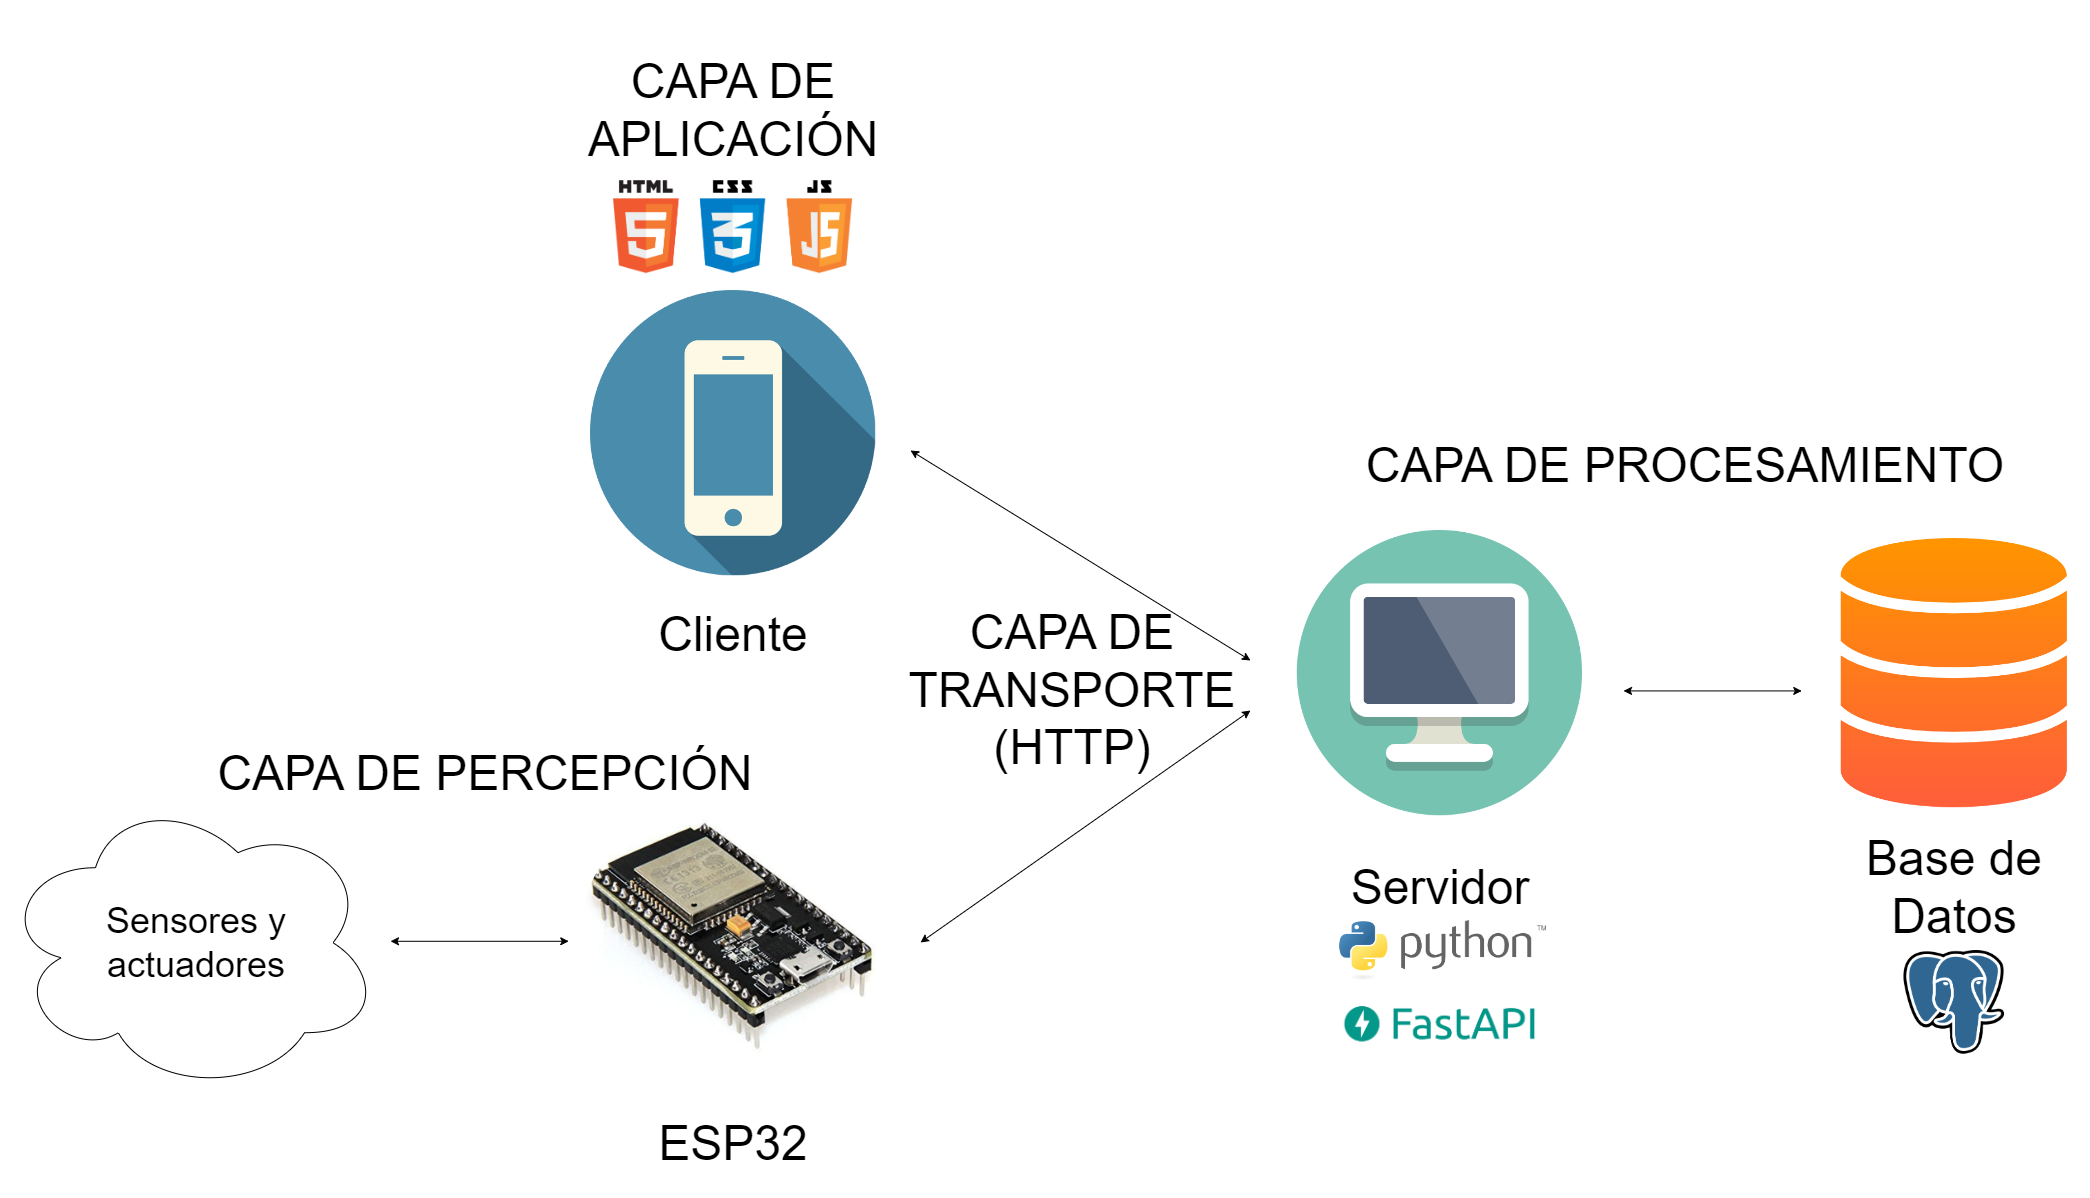
\includegraphics[width=0.75\linewidth]{imagenes//diagramas/Diagrama arquitectura.png}
    \caption{Arquitectura del proyecto}
    \label{fig:enter-label}
\end{figure}
A continuación se describirá en detalle los papeles de cada una de estas capas:
\newpage
\section{Capa de percepción}
También conocida como capa de sensores, es la capa más baja en la arquitectura IoT. Aquí es donde se encuentran los dispositivos y sensores que recopilan datos del entorno físico, como temperatura, presión, movimiento, luz, etc. Estos dispositivos pueden ser sensores, actuadores, medidores, entre otros.
\subsection{Sensores y actuadores}
Hemos hecho uso de diferentes tipos de sensores y de actuadores los cuales serán detallados a continuación:
\subsubsection{Sensores}
 Son los dispositivos de entrada de datos a la placa microcontroladora, estos recogen datos del exterior para poder entender que esta sucediendo en el exterior de la placa. 
 \begin{itemize}
    \item \textbf{Sensor de ultrasonidos:} Este sensor se utiliza para medir la distancia entre este y el objeto más cercano frente a él, para ello hace uso de ultrasonidos. Las dos orejas que se ven en el aparato envían (\textit{trigger}) y reciben (\textit{echo}) estas señales rebotan en el objeto, así podemos medir su lejanía. En el proyecto actual serán usados para poder detectar cuándo la puerta de una taquilla está abierta o cerrada y así poder iniciar el proceso de cierre solo cuando la puerta esté cerrada completamente y no pueda entorpecerse el funcionamiento de esta.
    \item \textbf{Sensor de humedad y temperatura DHT11:} El sensor de humedad y temperatura DHT11 recibe información de su entorno sobre la humedad y la temperatura de la sala en la que esté. Este será utilizado para poder interpretar la temperatura que hace en cada aula y poder saber si es necesario encender la calefacción o el aire acondicionado para que las condiciones del aula sean óptimas para poder impartir en ella clase y se optimice de la mejor manera el sistema de climatización del aula.
 \end{itemize}
\subsubsection{Actuadores}
\begin{itemize}
    \item \textbf{Servomotor sg90: }Este servomotor es un servo actuador que cuenta con una capacidad de rotación de 180º, suficiente para poder realizar la apretura y cierre de la puerta de la taquilla junto con la pieza impresa en impresora 3D solicitada a los docentes.
    \item \textbf{Buzzer}: El buzzer es un actuador que cuando recibe señal emite sonido, es utilizado para que el usuario de la taquilla sepa cuando se ha pulsado una tecla, así como para saber cuando la contraseña introducida ha sido correcta o errónea o cuando se está ejecutando el proceso de cierre de la taquilla.
    \item \textbf{Led}: Se implementará una luz led que indicará al usuario de eventos en la taquilla, en concreto, serán los mismos que en los que actúa el buzzer.
\end{itemize}
\subsubsection{Periféricos}
\begin{itemize}
    \item \textbf{Keypad:} pad de dimensiones 4x4 con el que podemos introducir la contraseña de la taquilla, actúa sobre 8 pines. Cada uno de ellos transmite la señal de su columna o fila correspondiente.
\end{itemize}
\subsection{ESP32}
\subsubsection{Introducción}
Para el desarrollo de la practica se ha utilizado un ESP32, que es es un microcontrolador de bajo costo y bajo consumo de energía que combina capacidades de conectividad Wi-Fi y Bluetooth. Fue desarrollado por la empresa Espressif Systems y se ha convertido en una opción popular para proyectos de Internet de las cosas (IoT) debido a su versatilidad y potencia. 
\\\\
También soporta diferentes protocolos de red, como TCP/IP, HTTP, HTTPS, MQTT y WebSocket, lo que facilita la integración con servicios en la nube y la comunicación con otros dispositivos en la red. Además de una amplia comunidad de desarrolladores que ofrecen bibliotecas y recursos para facilitar la programación y el desarrollo de proyectos. Se puede programar utilizando el entorno de desarrollo integrado (IDE) de Arduino. 
\\\\
Cuenta también con varias salidas GND y PWR así como un total de 34 pines digitales para la conectividad con sensores y actuadores. de los cuales usamos 2 para el sensor de ultrasonidos, 1 para el sensor DHT11, 1 para el servomotor SG90, 8 pines para el keypad, 1 para el buzzer y otro para el LED.
\subsubsection{Librerias}
Para poder utilizar todos los sensores y actuadores empleados para el desarrollo de esta practica hemos tenido que descargar varias librerías con las que poder controlarlos. Estas librerías que nos abren las puertas a los métodos para poder utilizar estos componentes se han descargado desde la IDE de Arduino y han sido creados por la extensa comunidad de este. Las librerías utilizadas son las siguientes:
\begin{itemize}
    \item \textbf{adafruit BusIO by adafruit:} Utilizado para el control general de componentes.
    \item \textbf{adafruit unified sensor by adafruit:} Utilizado para el control general de componentes.
    \item \textbf{DHT sensor library by adafruit:} Utilizada para controlar el sensor DHT11.
    \item \textbf{esp32Servo by kevin harrington, john k bennett:} Utilizada par controlar el servomotor.
    \item \textbf{keypad by mark stanley, alexander:} Utilizada para controlar el keypad.
    \item \textbf{RTClib by adafruit:} Utilizada para el uso del buzzer y Led.
    \item \textbf{WIFIManager by Tzapu:} Utilizada para la conectividad Wi-Fi.
    \item \textbf{Time by Michael Margolis:} Utilizada para el control de tiempos.
\end{itemize}
\subsection{NFC}
Para el manejo de los pedidos de la cafetería se hace uso de NFC o Near Field Communication (Comunicación de Campo Cercano, en español). Es una tecnología de comunicación inalámbrica de corto alcance que permite la transferencia de datos entre dispositivos compatibles en distancias muy cercanas, generalmente dentro de unos pocos centímetros.
\\\\
La tecnología NFC se basa en la tecnología RFID (Identificación por Radiofrecuencia) y utiliza ondas de radio de alta frecuencia para el intercambio de datos. La comunicación NFC se establece cuando dos dispositivos están suficientemente cerca, lo que puede ser al tocarlos o acercarlos uno al otro.
\\\\
Serán utilizados para el manejo de los pedidos de la cafetería como se ha mencionado antes, la cafetería contará con bandejas con NFC integrados que servirán para la comprobación de la recepción de un pedido por su dueño, este acercará el teléfono móvil a la bandeja para reconocer que es su pedido y podrá llevárselo para disfrutar de su almuerzo.
\section{Capa de transporte} 
Esta capa se encarga de la comunicación entre los dispositivos de la capa de percepción y la capa siguiente. Aquí se utilizan protocolos de comunicación como Wi-Fi, Bluetooth, Zigbee, LoRa, MQTT, HTTP, entre otros, para transmitir los datos recopilados por los dispositivos hacia la capa de procesamiento y análisis.
\\\\
En este nuevo proyecto hemos decidido abandonar MQTT, un protocolo que pese a su ligereza, no encaja como nos gustaría en esta nueva arquitectura que hemos propuesto para este proyecto. 
En su lugar, hemos optado por emplear \textit{llamadas HTTP}, que desde nuestro punto de vista, encajan perfectamente con las características de este proyecto, ya que es tan sencillo como llamar a un \textit{endpoint} mediante llamadas post de HTTP enviando un Json como contenido del mensaje y detectando la respuesta que nos envía el servidor. 
\\\\
Esto facilita las labores de comunicación ya que el propio servidor solo requiere disponer de los \textit{endpoints} a los que se llamará desde el microcontrolador para poder funcionar correctamente. Además, encaja a la perfección con la arquitectura de nuestro proyecto.
\\\\
En esta capa realizamos cuatro funciones de transporte elementales:
\begin{itemize}
    \item \textbf{Llamada para la apertura de la taquilla:} en el momento en el que el Arduino recibe 4 dígitos introducidos por el keypad, este realizara una llamada post al servidor, al endpoint \textit{abrir taquilla} en el que se especifica el id de la taquilla en cuestión así como la contraseña introducida que estará contenida dentro del Json a enviar. 
    \\ Una vez enviado, el servidor ejecuta dicho endpoint y devuelve un código de respuesta, se preveen 2 situaciones: la primera es que la contraseña introducida sea la correcta para la taquilla en la que se ha tecleado, en cuyo caso el servidor responderá con un código de OK (código 200) y se procederá a abrir la puerta de la taquilla. 
    \\ El otro caso es el contrario, que la contraseña no sea correcta, en este caso el servidor enviara un código de respuesta 400 que indica que algo ha salido mal, en este caso se inicia el procedimiento de error que le hace saber al usuario que ha fallado al introducir la contraseña.
    \item \textbf{Llamada para la comprobación de la calefacción:} cada 2 minutos el ESP32 comprobará de manera inteligente si es el momento óptimo para encender el sistema de climatización del aula mediante un Get.
    \item  \textbf{Actualización de la temperatura del aula: }cada 2 minutos se actualizará el valor de la temperatura de cada aula mediante las mediciones del sensor DHT.
    \item \textbf{Envío de datos de climatización al sistema: }Una vez terminada la climatización del aula se guardarán datos como el tiempo tardado en calentar el aula en la base de datos.
\end{itemize}
Para la realización del testing de estas llamadas hemos hecho uso de \textit{Postman}, al tratarse de llamadas a endpoints, el testing se ha simplificado significativamente con respecto al testing previo ya que se ha realizado de la misma manera a la que se ha realizado el testing del resto de llamadas que se hacen al servidor desde el Front end haciendo el testing más accesible y veloz.
\section{Capa de procesamiento} 
En esta capa, los datos recopilados por los dispositivos son procesados, analizados y transformados en información útil. Aquí se aplican algoritmos y técnicas de análisis de datos para extraer conocimientos, patrones y realizar acciones basadas en esos datos. 
\\\\
También se puede realizar algún nivel de procesamiento en tiempo real para tomar decisiones instantáneas.
Esta capa recoge todo el backend de nuestro proyecto, desde endpoints, base de datos y capa lógica del proyecto.
\\\\
En el capítulo \textit{5. Base de datos online} se explicará el modelo E/R y las tablas usadas en el sistema. En el capítulo \textit{6. Desarrollo de la API} se explicarán los distintos aspectos del backend.
\section{Capa de Aplicación}
Esta es la capa superior de la arquitectura IoT, donde se encuentran las aplicaciones y servicios que interactúan con los usuarios o con otros sistemas. Aquí se utilizan los datos y conocimientos obtenidos de las capas anteriores para ofrecer servicios, controlar dispositivos, generar informes, tomar decisiones, entre otras funcionalidades.
\\\\
En esta capa se encuentra todo el front-end del proyecto, esto implica los archivos html para mostrar la pagina web, javascript para implementar código dentro de los ficheros html y poder hacer llamadas a la capa de procesamiento y css para estilizar las páginas html. 
\\\\
Se trata de una aplicación web sencilla de utilizar para el usuario que implementa todas las funcionalidades del proyecto, en ella se puede reservar una taquilla, ver qué clases se están impartiendo en las diferentes aulas así como la temperatura que hace en ellas, y además es posible realizar pedidos en la cafetería y recogerlos.
\\\\
En el capítulo \textit{7. Diseño e implementación del front-end} se explicará con mayor detalle.

\chapter{Base de datos online} 
Para poder desarrollar el modelo E/R se ha empleado la herramienta \textit{pgModeler} debido a que permite de manera sencilla e intuitiva la creación del modelo.
\\
El modelo ha sufrido diversos cambios hasta llegar al modelo final. A continuación, se detallarán varias de las versiones implementadas que fueron descartadas hasta llegar a la definitiva.

\section{Modelo E/R: Versión 1}
Inicialmente se planteó una versión en la que, el horario en el que se impartía una asignatura era una columna de la tabla \textit{Asignatura}. Además, no existía ninguna relación entre \textit{Alumno} y \textit{Asignatura}. También se planteó incorrectamente la relación entre \textit{Producto} y \textit{Pedido}, ya que esta es una relación \textit{n:m}.

\begin{figure}[H]
    \centering
    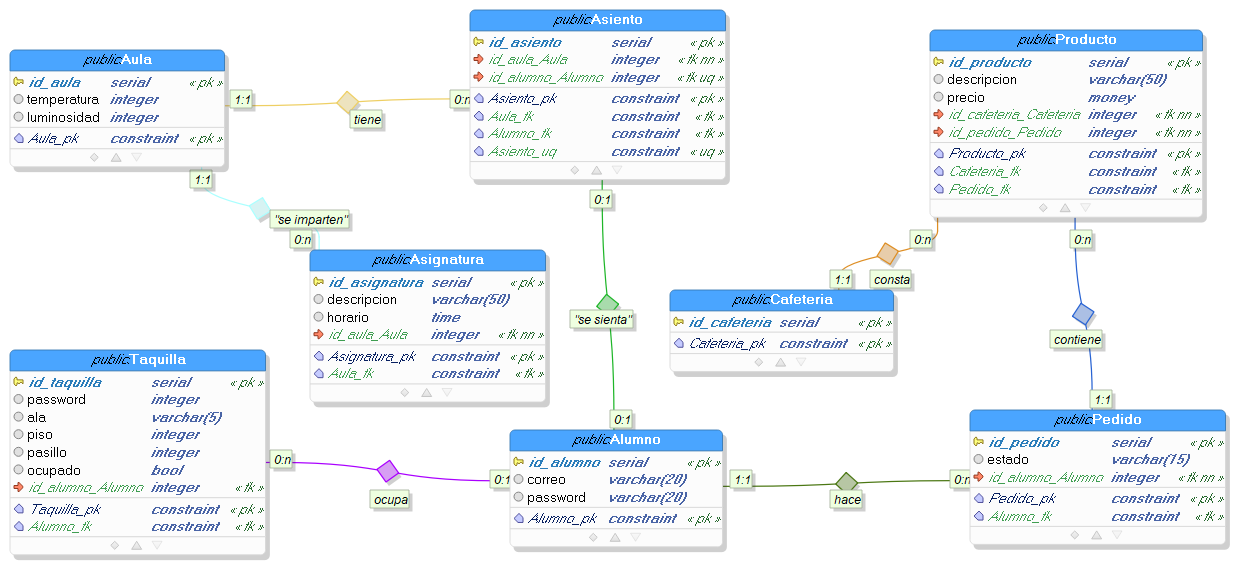
\includegraphics[scale = 0.5]{imagenes//base_de_datos/ImagenBD.png}
    \caption{Primera versión del modelo E/R}
    \label{fig:Figura4}
\end{figure}
\newpage
\section{Modelo E/R: Versión 2}
En esta versión podemos observar un modelo mucho más avanzado. Los principales cambios con respecto a la versión inicial son:

\begin{itemize}
    \item Creación de una nueva tabla \textit{Horario} para contemplar que una asignatura se pueda impartir en diferentes tramos horarios y en diferentes días lectivos.
    \item Relación \textit{Asignatura-Alumno}: dado que esta era una relación \textit{n:m}, se ha normalizado mediante la creación de la tabla \textit{Matricula}.
    \item Creación de una nueva tabla \textit{NFC} que será empleada para guardar el identificador de cada NFC que estará asignado a un pedido.
    \item Modificación de la tabla \textit{Cafetería}: en esta versión decidimos denominarla como \textit{Empleado} puesto que la Escuela Politécnica Superior tiene una única cafetería. Con esta tabla creamos un nuevo rol que será el encargado de preparar los productos para los pedidos.
    \item Relación \textit{Pedido-Producto}: dado que esta era una relación \textit{n:m}, se ha normalizado mediante la creación de la tabla \textit{Pedido\_Producto}.
    \item Añadidas nuevas columnas en la tabla \textit{Aula} como laboratorio, planta, ala, ...
    \item Se ha eliminado la relación \textit{Asignatura-Aula} y se han añadido dos nuevas relaciones: \textit{Asignatura-Horario} y \textit{Horario-Aula}.
\end{itemize}  

\begin{figure}[H]
    \centering
    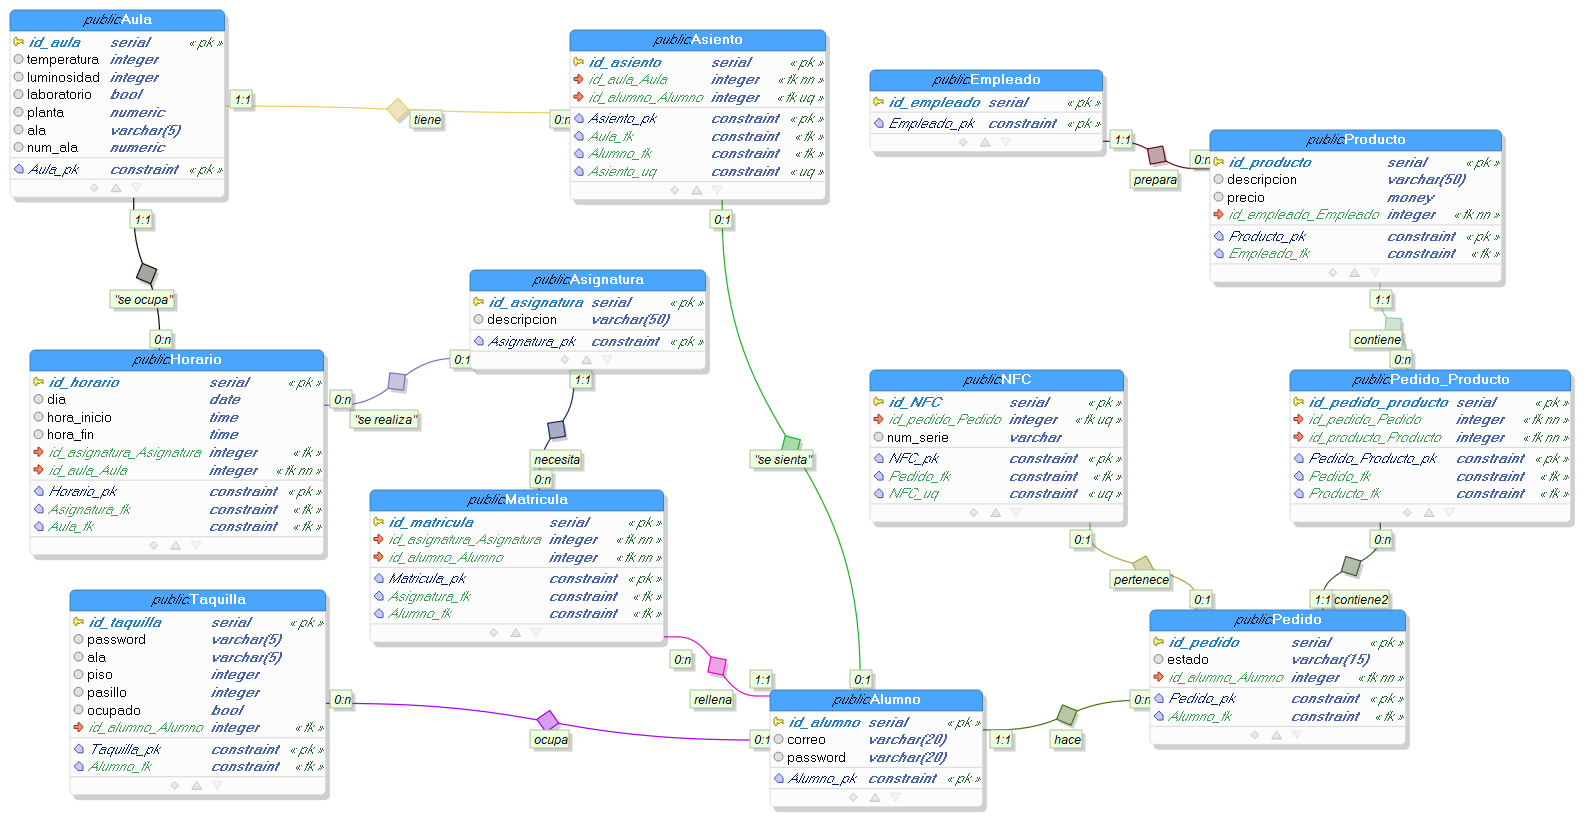
\includegraphics[scale = 0.4]{imagenes//base_de_datos/ImagenBD2.png}
    \caption{Segunda versión del modelo E/R}
    \label{fig:Figura3.4.2}
\end{figure}

\section{Modelo E/R: Versión 3}
Esta es la última y definitiva versión del modelo E/R del sistema. Los principales cambios con respecto a la anterior versión son:
\begin{itemize}
    \item Se ha añadido una nueva tabla \textit{Histórico\_Aula}: en esta tabla se almacena la temperatura a la que se encontraba el aula así como el tiempo que tarda en llegar a la temperatura óptima.
    \item Añadidas nuevas columnas en \textit{Producto}: se ha añadido tanto un breve detalle del producto como una imagen de este.
\end{itemize} 

\begin{figure}[H]
    \centering
    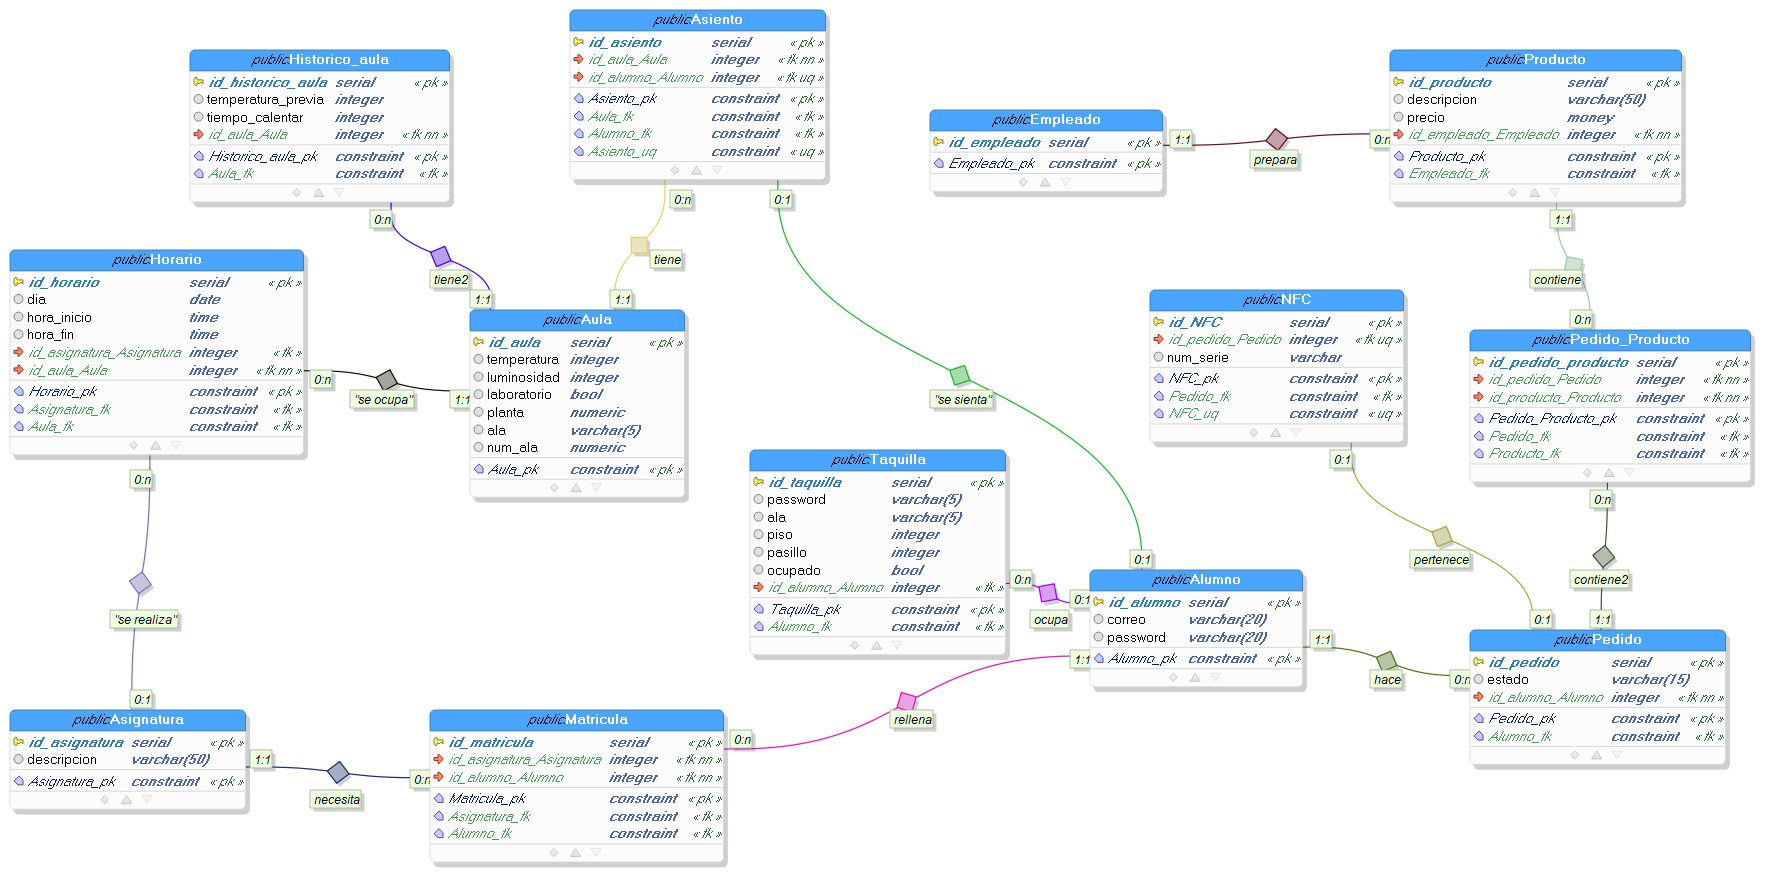
\includegraphics[scale = 0.35]{imagenes//base_de_datos/ImagenBD3.png}
    \caption{Última versión del modelo E/R}
    \label{fig:Figura3.4.3}
\end{figure}

\section{Esquema de tablas}
A continuación, detallaremos las distintas tablas del modelo E/R así como sus distintos atributos:
\begin{itemize}
    \item\textbf{Alumno}: es el principal usuario de nuestro sistema. Dentro de esta tabla almacenaremos:
    \begin{itemize}
        \item \textbf{Id\_alumno}: se trata de un serial que nos permitirá identificar a cada alumno ya que es \textit{PRIMARY\_KEY}.
        \item \textbf{Correo}: se trata del propio correo electrónico del alumno.
        \item \textbf{Password}: se trata de la contraseña asociada al correo electrónico del alumno.
        \\\\\\
    \end{itemize}
    
    \item\textbf{Taquilla}: en esta tabla se almacenarán las principales características de cada una de las taquillas de la Escuela Politécnica Superior. Estas características son:
    \begin{itemize}
        \item\textbf{Id\_taquilla}: se trata de un serial que nos permitirá identificar cada taquilla ya que es \textit{PRIMARY\_KEY}.
        \item \textbf{Password}: se trata de la contraseña asociada a la taquilla para que esta se pueda abrir correctamente.
        \item \textbf{Ala}: dado que la escuela se divide en distintas alas (Este, Norte, Oeste y Sur), en este campo almacenaremos la ubicación.
        \item \textbf{Piso}: almacenaremos también el piso en el que se encuentra cada taquilla.
        \item \textbf{Pasillo}: en cada ala hay dos pasillos distintos, por lo que almacenaremos el pasillo en el que se encuentra la taquilla.
        \item \textbf{Ocupado}: se trata de un valor booleano que nos indicará si dicha taquilla pertenece o no a un alumno.
        \item \textbf{Id\_alumno\_alumno}: como las taquillas se relacionan con los alumnos, en caso de que una taquilla este ocupada se almacenará el id del alumno que la ha reservado.
        \\
    \end{itemize}
    \item \textbf{Aula}: en esta tabla se almacenarán las principales características de cada aula. Estas son:
    \begin{itemize}
        \item\textbf{Id\_aula}: se trata de un serial que nos permitirá identificar cada aula ya que es \textit{PRIMARY\_KEY}.
        \item \textbf{Temperatura}: almacenaremos la temperatura de cada aula gracias a un sensor de temperatura.
        \item \textbf{Luminosidad}: al igual que la temperatura, también se almacenará la luminosidad del aula.
        \item \textbf{Laboratorio}: almacenaremos si el aula es o no un laboratorio.
        \item \textbf{Planta}: al igual que en las taquillas, almacenaremos en qué planta se encuentra el aula.
        \item \textbf{Ala}: dado que la escuela se divide en distintas alas (Este, Norte, Oeste y Sur), en este campo almacenaremos la ubicación.
        \item \textbf{Num\_ala}: almacenaremos cuál es el número de aula.
        \\
    \end{itemize} 
    \item  \textbf{Historico\_Aula}: para poder saber cuánto tiempo se necesita para que la temperatura de un aula sea la óptima, hemos creado esta tabla. En ella se guardarán las siguientes características
    \begin{itemize}
        \item\textbf{Id\_Historico\_Aula}: se trata de un serial que nos permitirá identificar cada histórico de un aula ya que es \textit{PRIMARY\_KEY}.
        \item \textbf{Temperatura\_previa}: se almacenará la temperatura a la que se encontraba el aula antes de haber llegado a su temperatura óptima.
        \item \textbf{Tiempo\_calentar}: se almacenará también el tiempo que se ha tardado en llegar desde la temperatura previa a la temperatura óptima.
        \item \textbf{Id\_aula\_aula}: como los históricos se relacionan con las aulas, almacenamos el id del aula donde se ha realizado un cambio de temperatura.
        \\
    \end{itemize} 
    \item  \textbf{Asignatura}: dado que en la Escuela Politécnica Superior se imparten distintas asignaturas, almacenaremos las siguientes características:
    \begin{itemize}
        \item\textbf{Id\_asignatura}: se trata de un serial que nos permitirá identificar cada asignatura ya que es \textit{PRIMARY\_KEY}.
        \item \textbf{Descripción}: se trata del nombre de la asignatura impartida.
        \\
    \end{itemize} 
    \item  \textbf{Horario}: para saber cuándo se ocupa una determinada aula, usaremos los horarios. En esta tabla se almacenan:
    \begin{itemize}
        \item\textbf{Id\_horario}: se trata de un serial que nos permitirá identificar cada horario ya que es \textit{PRIMARY\_KEY}.
        \item \textbf{Día}: almacenaremos el día en el que se imparte una asignatura.
        \item \textbf{Hora\_inicio}: almacenaremos la hora en la que empieza una asignatura.
        \item \textbf{Hora\_fin}: almacenaremos la hora en la que finaliza una asignatura.
        \item \textbf{Id\_asignatura\_asignatura}: como los horarios se relacionan con las asignaturas, almacenamos el id de la asignatura que se imparte en dicho horario.
        \item \textbf{Id\_aula\_aula}: como los horarios se relacionan con las aulas, almacenamos el id del aula donde se imparte la asignatura en dicho horario.
        \\
    \end{itemize} 
    \item  \textbf{Empleado}: para la implementación de la parte de la cafetería hemos creado un usuario que se encarga de preparar los distintos productos. Almacenamos en esta tabla la siguiente característica:
    \begin{itemize}
        \item\textbf{Id\_empleado}: se trata de un serial que nos permitirá identificar cada empleado de la cafetería ya que es \textit{PRIMARY\_KEY}.
        \\
    \end{itemize} 
    \item  \textbf{Producto}: la cafetería ofrece diversos productos que se encuentran almacenados en la base de datos en esta tabla. Las características de cada producto son:
    \begin{itemize}
        \item\textbf{Id\_producto}: se trata de un serial que nos permitirá identificar cada producto ya que es \textit{PRIMARY\_KEY}.
        \item \textbf{Descripción}: se almacenará el nombre de cada producto que se ofrece en la cafetería.
        \item \textbf{Precio}: se almacenará el precio por unidad de cada producto.
        \item \textbf{Id\_empleado\_empleado}: como los productos se relacionan con los empleados de la cafetería, almacenamos el id del empleado que prepara cada producto.
        \\\\\\
    \end{itemize} 
    \item \textbf{Pedido}: al poder realizar un pedido de la cafetería desde la página web, almacenaremos los siguientes datos en esta tabla:
    \begin{itemize}
        \item\textbf{Id\_pedido}: se trata de un serial que nos permitirá identificar cada pedido ya que es \textit{PRIMARY\_KEY}.
        \item \textbf{Estado}: para saber si nuestro pedido está listo observaremos este valor:
        \begin{itemize}
            \item \textbf{0}: nos indica que la petición del pedido ha sido recibida y está pendiente de aprobarse.
            \item \textbf{1}: nos indica que el pedido ha sido aceptado y se está preparando en la cocina.
            \item \textbf{2}: nos indica que el pedido ha sido preparado correctamente y está listo para ser recogido.
            \item \textbf{3}: nos indica que el pedido ha sido recogido y por tanto se está consumiendo.
            \item \textbf{4}: nos indica que el pedido ha sido consumido y por tanto finalizado.
            \item \textbf{5}: nos indica que el pedido se ha cancelado.
        \end{itemize}
        \item \textbf{Id\_alumno\_alumno}: como los pedidos se relacionan con los alumnos, se almacenará el id del alumno que ha realizado el pedido. 
    \\
    \end{itemize} 
    \item  \textbf{Pedido\_Producto}: esta tabla, tal y como se ha explicado en el modelo E/R, surge porque la relación entre \textit{Pedido} y \textit{Producto} es \textit{n:m}. Esta tabla se compone de:
    \begin{itemize}
        \item\textbf{Id\_pedido\_producto}: se trata de un serial que nos permitirá identificar cada pedido\_producto ya que es \textit{PRIMARY\_KEY}.
        \item\textbf{Id\_pedido\_pedido}: nos permitirá identificar el pedido.
        \item\textbf{Id\_producto\_producto}: nos permitirá identificar el producto.
        \\
    \end{itemize} 
    \item  \textbf{NFC}: en la cafetería emplearemos los NFCs para poder recoger los pedidos. Esta tabla se compone de:
    \begin{itemize}
        \item\textbf{Id\_NFC}: se trata de un serial que nos permitirá identificar cada NFC ya que es \textit{PRIMARY\_KEY}.
        \item\textbf{Id\_pedido\_pedido}: nos permitirá identificar el pedido.
        \item\textbf{Num\_serie}: cada NFC lleva asociado un número de serie por lo que almacenaremos dicho valor.
    \\
    \end{itemize} 
\end{itemize} 

\section{Tablas extra}
Se puede observar que las tablas \textit{Asiento} y \textit{Matrícula} no se usan en el sistema actual. Esto se debe a que nuestro proyecto es escalable y serían futuras mejoras. Por ejemplo, la tabla \textit{Asiento} almacenaría gracias a NFC donde está situado un alumno en el Aula.
\newpage
\section{Vistas}
Además de las tablas mencionadas en los apartados anteriores, dentro de la base de datos podemos observar distintas vistas:
\begin{itemize}
    \item \textbf{Vista asignaturas}: dentro de esta vista podremos observar las distintas características de una asignatura así como la clase donde se imparte y en qué horario.
    \begin{figure}[H]
        \centering
        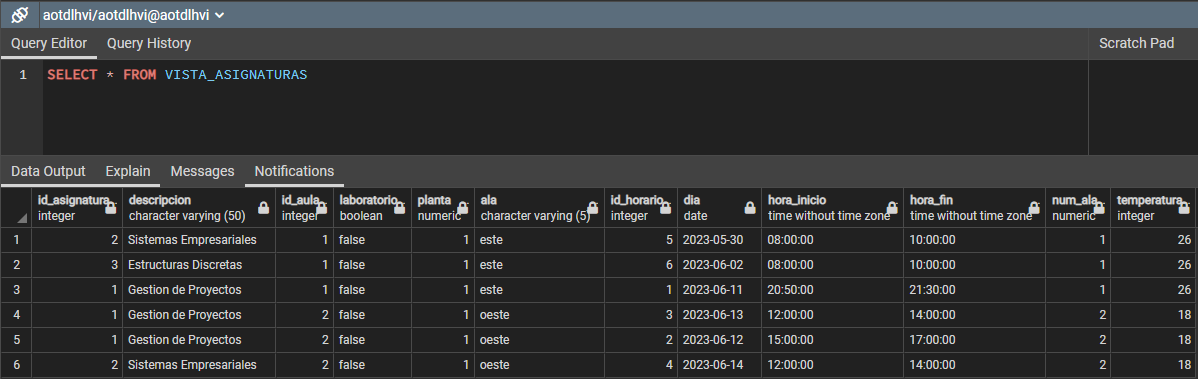
\includegraphics[scale = 0.55]{imagenes//base_de_datos/Vista_asignaturas.png}
        \caption{Vista asignaturas}
        \label{fig:Figura}
    \end{figure}
    
    \item \textbf{Vista pedido estrella}: dentro de esta vista podremos observar los distintos productos que se encuentran en los pedidos junto a la descripción de estos pedidos y al identificador del alumno.
    \begin{figure}[H]
        \centering
        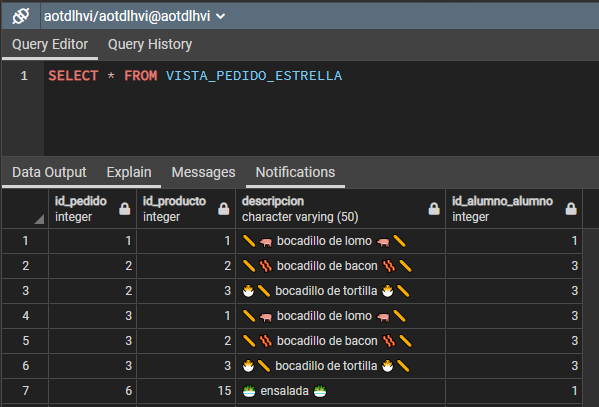
\includegraphics[scale = 0.75]{imagenes//base_de_datos/Vista_pedido_estrella.png}
        \caption{Vista pedido estrella}
        \label{fig:Figura}
    \end{figure}
    \newpage
    \item \textbf{Vista pedidos}: dentro de esta vista podremos observar todos los productos que ha ordenado un alumno en un único pedido.
    \begin{figure}[H]
        \centering
        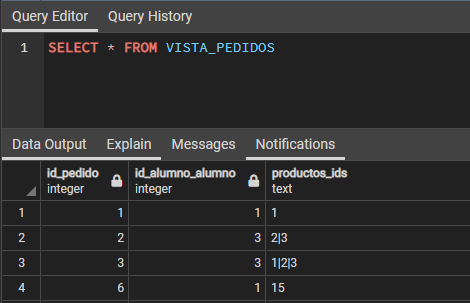
\includegraphics[scale = 0.65]{imagenes//base_de_datos/Vista_pedidos.png}
        \caption{Vista pedidos}
        \label{fig:Figura}
    \end{figure}
    
    \item \textbf{Vista resumen aula}: dentro de esta vista obtendremos cuál es la próxima asignatura que se imparte en un aula y si es necesario actuar en ella para llegar a conseguir la temperatura óptima antes de que empiece la asignatura.
    \begin{figure}[H]
        \centering
        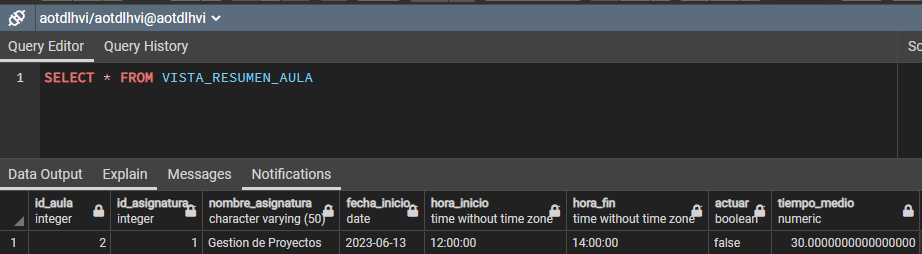
\includegraphics[scale = 0.65]{imagenes//base_de_datos/Vista_resumen_aula.png}
        \caption{Vista resumen aula}
        \label{fig:Figura}
    \end{figure}
    \item Dentro de esta vista tenemos las siguientes columnas:
    \begin{itemize}
        \item \textbf{id\_aula:} identificador de un aula.
        \item \textbf{id\_asignatura:} identificador de una asignatura.
        \item \textbf{nombre\_asignatura:} nombre de la asignatura.
        \item \textbf{fecha\_inicio:} fecha de inicio de una asignatura en un aula.
        \item \textbf{hora\_inicio:} hora de inicio de una asignatura en un aula.
        \item \textbf{hora\_fin:} La hora de finalización de una asignatura en un aula.
        \item \textbf{actuar:} esta columna utiliza una expresión condicional CASE para determinar si se debe actuar en base a ciertas condiciones. Si la fecha de inicio es igual a la fecha actual \textit{(CURRENT\_DATE)} y la hora de inicio es posterior o igual a la hora actual \textit{(CURRENT\_TIME)}, o si la fecha de inicio es posterior a la fecha actual, entonces el valor de actuar será \textit{true}. De lo contrario, será \textit{false}.
        \item \textbf{tiempo\_medio:} tiempo medio calculado para un aula específica, que se obtiene a partir de una subconsulta.
    \end{itemize}
    \item Como se puede observar en la \textit{Figura 5.8.}, la vista se construye mediante la unión de dos subconsultas anidadas:
    \begin{itemize}
        \item La primera subconsulta (pc) \textbf{obtiene información} sobre las aulas, asignaturas y horarios.
        \item La segunda subconsulta (ta) \textbf{calcula el tiempo medio} para cada aula a partir de un historial de aulas
    \end{itemize}
    \begin{figure}[H]
        \centering
        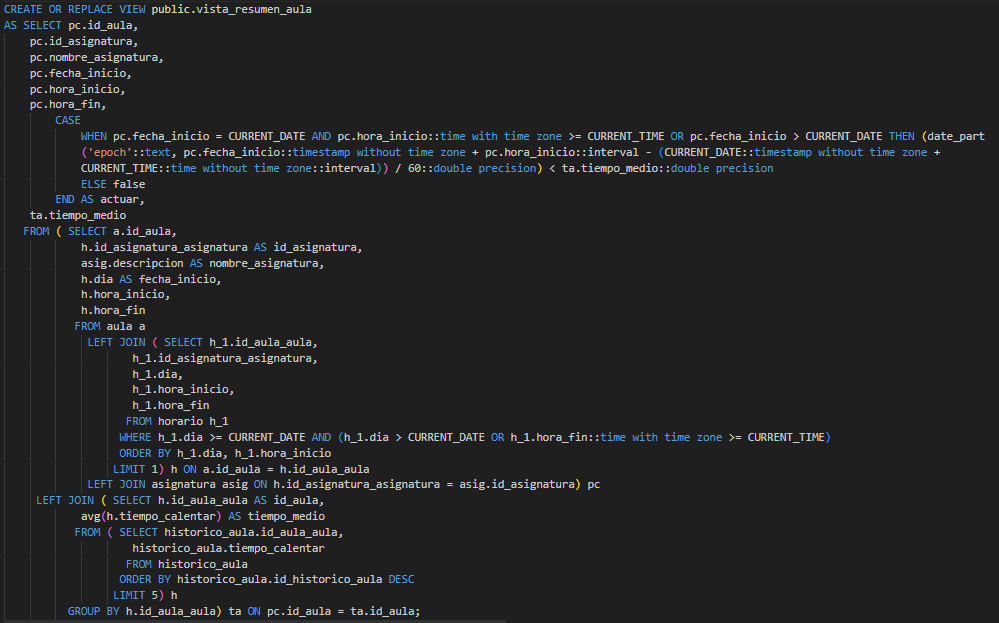
\includegraphics[scale = 0.65]{imagenes//base_de_datos/Codigo_vista_resumen_aula.png}
        \caption{Vista resumen aula}
        \label{fig:Figura}
    \end{figure}
    
\end{itemize}
\newpage
\section{Instalación y configuración}
En cuanto a la instalación y configuración de la propia base de datos, hemos optado por obtener una online gratuita hosteada de manera remota. Se trata de una base de datos en PostgreSQL de elephantsql (\url trumpet.db.elephantsql.com) que permite 5 conexiones simultáneas y tiene un almacenamiento de hasta 20MB.
\\\\
Para acceder a ella hemos optado por utilizar un gestor de bases de datos. En nuestro caso hemos utilizado dos diferentes, dependiendo del miembro del grupo: \textit{pgAdmin4} y \textit{Dbeaver}. Dentro del gestor, crearemos un servidor con las credenciales que hemos obtenido. Una vez verificadas, podremos acceder a nuestra base de datos sin problemas.
\\\\
Para insertar las distintas tablas que hemos mencionado anteriormente usaremos el código SQL que podemos exportar desde \textit{pgModeler}. Cuando tengamos este código lo copiaremos y pegaremos en la propia base de datos. Una vez insertadas todas las tablas hemos añadido algunos datos de prueba que se encuentran en el fichero \textit{DatosBD3.sql}.


\chapter{Desarrollo de la API}
Como se ha detallado anteriormente, este apartado ha sido desarrollado por completo utilizando el \textit{framework} de \textit{FastApi} para el lenguaje \textit{Python}. Un desarrollo de un \textit{Backend} complejo y sofisticado siempre es una tarea de alta dificultad, sin embargo, gracias a utilizar este \textit{framework}, nuestro trabajo se ha simplificado y acelerado en gran medida.
\\
A continuación se detallarán aspectos importantes a destacar de la implementación realizada.
\section{Estructura clara y organizada}
Desde el inicio del proyecto, hicimos hincapié en la importancia de contar con una estructura de código clara y organizada, que permitiera localizar rápidamente cualquier aspecto del mismo.
\\

En este contexto, la implementación adoptada se basa en un archivo principal denominado \texttt{main.py}, el cual contiene la aplicación \textit{FastAPI}. A este archivo se agregan todos los nodos terminales que se encuentran en la carpeta \textit{endpoints}. Estos endpoints se encuentran distribuidos en varios archivos \textit{.py}, clasificados de acuerdo con el aspecto de la \textit{API} que manejan. Por ejemplo, se pueden encontrar archivos como \textit{taquillas.py}, \textit{productos.py}, entre otros.
\\

Además de la organización de los endpoints, esta implementación también proporciona una forma sencilla de agregar todos los archivos necesarios para mostrar la interfaz de usuario (\emph{frontend}). Esto implica que la estructura del proyecto permite incorporar de manera eficiente los archivos relevantes para la interfaz de usuario, facilitando así su desarrollo y mantenimiento.
\\

A continuación se muestra un diagrama de la estructura utilizada:
\begin{figure}[H]
    \centering
\begin{tikzpicture}[
  level 1/.style={sibling distance=60mm},
  level 2/.style={sibling distance=30mm},
  level 3/.style={sibling distance=20mm}
]
\node {main.py}
  child {node {endpoints}
    child {node {taquillas.py}}
    child {node {productos.py}}
    child {node {sesion.py}}
    child {node {aulas.py}}
    child {node {...}}
  };
\end{tikzpicture}
\caption{Diagrama de la estructura del proyecto}
\label{fig:arbol_estructura}
\end{figure}

\section{Proceso de levantamiento local del servidor}
Como ya se ha mencionado anteriormente, una de las grandes ventajas que ofrece este \textit{setup} es la trivial replicación del servidor en cualquier máquina.\\
Para ello, en primer lugar se debe crear un entorno virtual de Python ejecutando:
\begin{verbatim}
    python -m venv env
\end{verbatim}
Tras la creación de este entorno virtual, se debe activar el mismo ejecutando:
\begin{verbatim}
    env\Scripts\activate.bat
\end{verbatim}
Una vez terminado ese paso, se deberá cargar el listado de requisitos localizado en \texttt{requirements.txt}. Para ello se deberá ejecutar
\begin{verbatim}
    pip install -r requirements.txt
\end{verbatim}
Finalizado este paso, ya tendremos todo listo para poder levantar el servidor sin problema. Para ello bastará con utilizar el siguiente comando de uvicorn:
\begin{verbatim}
    uvicorn --app-dir=BACK/ main:app --host 0.0.0.0 --reload
\end{verbatim}
Ya tendremos el servidor lanzado y podemos ver cómo se actualiza en tiempo real con cada cambio que realicemos en el código. Esto es gracias a haber escrito el argumento \texttt{--reload}.\\
Al haber especificado el host 0.0.0.0, podremos acceder al servidor desde cualquier dispositivo conectado en la misma red local.
Para cerrar el servidor se podrá utilizar la combinación de teclas \texttt{Ctrl+C}.\\

Una vez configurado el entorno, podremos levantar el servidor simplemente activando el entorno y utilizando el comando de uvicorn.\\
Sin embargo, se ha simplificado este proceso mediante un archivo de lotes llamado \texttt{levantar.bat}, que ya se encarga de hacer todos los pasos mencionados anteriormente.\\

En resumen, una vez configurado todo, levantar el servidor será tan simple como escribir en la terminal \texttt{"levantar"}.

\section{Túneles de CloudFlare}
Pese a que pueda parecer no tener gran utilidad debido a la sencillez que tiene el levantar localmente el servidor, los túneles de CloudFlare han resultado ser una herramienta vital para el desarrollo del proyecto.\\
Un túnel de Cloudflare, también conocido como Cloudflare Tunnel, es una solución que permite establecer una conexión segura y cifrada entre un servidor local y la red de Cloudflare. Básicamente, crea un canal seguro a través de Internet para transmitir el tráfico entre el servidor local y la infraestructura de \textit{Cloudflare}.\\
De esta manera, será muy sencillo levantar el servidor y compartirlo a personas ajenas a la red local, sin requerir a la creación de una \textit{VPN}.\\

En momentos en los que alguna persona tenía problemas para levantar el servidor, esta herramienta ha permitido poder seguir accediendo sin problema al servidor de otro compañero.\\

Además, para realizar las lecturas de ficheros NFC, por motivos de seguridad, es estrictamente necesario contar con una certificación \textit{SSL}. Al levantar el servidor localmente, no se contará con esta certificación, y el protocolo utilizado será HTTP básico. Gracias a los túneles de CloudFlare, se puede disponer de este certificado de manera totalmente gratuita, permitiendo así poder realizar las labores de lectura de estos dispositivos.

\begin{figure}[H]
    \centering
    
\includegraphics[width=0.75\linewidth]{imagenes//diagramas/diagrama_cloudflare.png}
    \caption{Diagrama del túnel de Cloudflare}
    \label{fig:enter-label}
\end{figure}
Para facilitar lo más posible la inicialización de túneles, se ha creado un archivo por lotes llamado \texttt{"tunel.bat"} que automáticamente se encarga de crear el túnel con la configuración necesaria.
\section{Manejo de errores}
Se ha implementado un sistema que permite lanzar errores que se le pueden mostrar al cliente de manera detallada; donde se le muestra el código de estado de la llamada \textit{HTTP}, junto con un mensaje detallando la causa del problema. La mayor complicación ha sido implementar el sistema haciendo que en el momento en el que se quiera mandar dicha respuesta al cliente, se interrumpa toda la ejecución y se devuelva únicamente el error especificado.

\section{Impresión interrumpida}
El método de depuración \texttt{printerrupt()} ofrece una solución eficiente para la depuración de nuestra \textit{API}.

El método \texttt{printerrupt()} permite interrumpir rápidamente la ejecución del programa y devuelve al cliente una cadena de texto plano especificada como argumento. Esta función resulta especialmente útil en situaciones en las que es difícil determinar la causa de un error en un momento determinado. Al proporcionar una forma de interrumpir la ejecución y obtener información en forma de texto plano, este método simplifica el proceso de identificación y resolución de cualquier tipo de error o fallo (\emph{bug}).

El uso de \texttt{printerrupt()} permite una depuración más eficiente al proporcionar una herramienta que ayuda a acotar el problema en cuestión. Al interrumpir la ejecución y enviar una respuesta al cliente, se facilita la identificación de puntos críticos en el código y se agiliza la solución de problemas.
\section{Utilidades para la base de datos}
Se han creado una serie de métodos que facilitan muy notoriamente el manejo de las conexiones a la base de datos donde se almacenan todos los datos.

Entre estos métodos destacan:
\begin{itemize}
    \item \texttt{realizar\_insercion}:
    \\
    Realiza la inserción de datos en una tabla de la base de datos, simplemente pasándole como argumentos el nombre de la tabla y un diccionario (\textit{JSON}) cuyos campos serán las columnas de la tabla. El método inteligentemente realiza una serie de verificaciones previas para asegurar que todo funcionará correctamente y cuenta con un manejo de errores detallado. A continuación, se muestran los pasos que sigue este método:

\begin{enumerate}
    \item Establece una conexión a la base de datos utilizando una función llamada \texttt{get\_connection()}.
    
    \item Verifica si la tabla especificada existe en la base de datos. Para ello, ejecuta una consulta de selección limitada a un solo registro en la tabla. Si la consulta arroja un error, se interpreta como que la tabla no existe y se genera un mensaje de error.
    
    \item Determina el nombre de la columna que actúa como clave primaria en la tabla. Esto se hace consultando el esquema de la base de datos y buscando la columna que tiene la restricción de ``\textit{PRIMARY KEY}".
    
    \item Verifica que la columna de la clave primaria no se haya proporcionado en el diccionario de datos o que su valor sea `\textit{None}`. Si se proporciona o su valor no es `\textit{None}`, se genera un mensaje de error. Los IDs de la base de datos implementada son del tipo Serial y se establecen automáticamente, por lo que no se deben enviar a la hora de realizar inserciones en la base de datos.
    
    \item Obtiene los nombres de todas las columnas de la tabla desde el esquema de la base de datos.
    
    \item Revisa que todas las columnas enviadas en el diccionario de datos existan en la tabla. Si alguna columna no existe, se genera un mensaje de error.
    
    \item Elimina las columnas de la lista que no están presentes en el diccionario de datos. Esto asegura que solo se inserten los valores para las columnas proporcionadas.
    % Aquellos que no estén se insertarán como nulos, siempre y cuando la tabla lo permita.
    
    \item Verifica que no falten campos requeridos que no pueden ser nulos en la base de datos. Esto se hace consultando los campos no nulos de la tabla y comparándolos con los campos proporcionados en el diccionario de datos. Si falta algún campo requerido, se genera un mensaje de error.
    
    \item Agrega `\textit{None}` como valor para las columnas que no están presentes en el diccionario de datos. Esto garantiza que se inserten `\textit{NULL}` en esas columnas.
    
    \item Construye una consulta de inserción automáticamente utilizando el nombre de la tabla y las columnas correspondientes. La columna de la clave primaria se omite en esta consulta por lo que se mencionó anteriormente.
    
    \item Ejecuta la consulta de inserción en la base de datos utilizando una función llamada `\texttt{insertar\_datos\_conexion()}`. Si ocurre un error de integridad debido a una violación de clave primaria, se genera un mensaje de error. Realmente, no debería haberlo nunca, pero pese a ello, se maneja dicho error.
    
    \item Obtiene el valor de la clave primaria del nuevo registro insertado utilizando una consulta que obtiene el valor actual de la secuencia de la clave primaria.
    
    \item Cierra la conexión a la base de datos.
    
    \item Retorna el valor de la clave primaria del nuevo registro insertado.
\end{enumerate}
En resumen, este método se encarga de realizar la inserción de datos en una tabla de una base de datos creando inteligentemente una consulta procesada. Esto se realiza verificando la existencia de la tabla, la validez de los datos proporcionados, la presencia de campos requeridos y la integridad de la clave primaria. Además, se encarga de manejar los mensajes de error y retorna el valor de la clave primaria del nuevo registro.

\item \texttt{realizar\_actualizacion}
Este método, de manera similar al anterior, se encarga de realizar una actualización en una tabla de una base de datos recibiendo únicamente el nombre de la tabla, el id del registro y un diccionario con aquellos campos que se deseen actualizar. Este método realiza la actualización tras verificar y manejar cualquier tipo de problema. A continuación, se detallan los pasos que sigue este método:

\begin{enumerate}
    \item Establece una conexión a la base de datos utilizando una función llamada `\texttt{get\_connection()}`.
    \item Verifica si la tabla especificada existe en la base de datos. Para ello, ejecuta una consulta de selección limitada a un solo registro en la tabla. Si la consulta arroja un error, se interpreta como que la tabla no existe y se genera un mensaje de error.
    \item Determina el nombre de la columna que actúa como clave primaria en la tabla. Esto se hace consultando el esquema de la base de datos y buscando la columna que tiene la restricción de "PRIMARY KEY".
    \item Verifica que la columna de la clave primaria no se haya enviado en el diccionario de datos y que el parámetro `id` no sea `None`. Si se envía la columna o `id` es `None`, se genera un mensaje de error.
    \item Obtiene los nombres de todas las columnas de la tabla desde el esquema de la base de datos.
    \item Verifica que exista un registro en la tabla con el valor de clave primaria especificado en el parámetro `id`. Si no existe un registro con ese valor de clave primaria, se genera un mensaje de error.
    \item Verifica que todas las columnas enviadas en el diccionario de datos existan en la tabla. Si alguna columna no existe, se genera un mensaje de error.
    \item Verifica que los campos con valor `None` puedan ser nulos en la base de datos. Esto se hace consultando los campos no nulos de la tabla y comparándolos con los campos y sus valores proporcionados en el diccionario de datos. Si se intenta asignar un valor `None` a un campo no nulo, se genera un mensaje de error.
    \item Construye la consulta de actualización y los valores a actualizar. Las columnas y sus respectivos valores se obtienen del diccionario de datos, excluyendo la columna de la clave primaria y las columnas que tienen un valor `None`. La consulta de actualización se construye utilizando la sintaxis SQL adecuada.
    \item Ejecuta la consulta de actualización en la base de datos utilizando una función llamada `\texttt{actualizar\_datos\_conexion()}`. Si ocurre un error de integridad debido a una violación de clave primaria, se genera un mensaje de error.
    \item Cierra la conexión a la base de datos.
    \item Retorna el valor del parámetro `id`.
\end{enumerate}

En resumen, este método se encarga de realizar una actualización en una tabla de una base de datos, verificando la existencia de la tabla, la validez de los datos proporcionados, la presencia de la clave primaria y las columnas, y la posibilidad de asignar valores `\textit{None}` a campos nulos. Además, se encarga de manejar los mensajes de error y retorna el valor del parámetro `id`.
\end{itemize}

\section{Implementación de envío de emails}
En el fichero \textit{correos.py} se puede observar toda la lógica relacionada con la mensajería a través de correo electrónico.\\
Para llevar a cabo este proceso, se han utilizado las librerías \textit{smtplib} y \textit{email}.\\
Tras la creación de una cuenta de Google que se encargará de enviar estos mensajes, se activó la verificación en dos pasos para poder obtener una \textit{contraseña de aplicación}. Gracias a esta contraseña, se ha realizado el inicio de sesión en el sistema \textit{SMTP} de \textit{Google} con el cual podemos enviar cualquier tipo de mensaje por correo.\\
Simplemente debemos preparar un email, el cual puede incluso incorporar \textit{HTML}, imágenes y estilos.\\
Finalmente, al indicarle los destinatarios, la función \texttt{enviar\_correo} realizará las acciones necesarias para finalizar el proceso.

En total se envían cuatro emails en la plataforma:
\begin{itemize}
    \item \textbf{Email de bienvenida:}
    Tras registrarse, el alumno será testigo de la recepción de un correo en su bandeja de entrada donde se le da la bienvenida a la plataforma de SmartUni, tal y como se contempla a continuación:
    \begin{figure}[H]
        \centering
        
\includegraphics[width=0.8\linewidth]{imagenes//emails/email_bienvenida.png}
        \caption{Email de bienvenida al registrarse}
        \label{fig:enter-label}
    \end{figure}
    \item \textbf{Email de confirmación de reserva de taquilla:}
    Cuando un alumno realice la reserva de una taquilla, obtendrá un correo de verificación de la misma, en el cuál podrá consultar todos los datos de esta, incluida la contraseña necesaria para acceder a la taquilla.
    \begin{figure}[H]
        \centering
        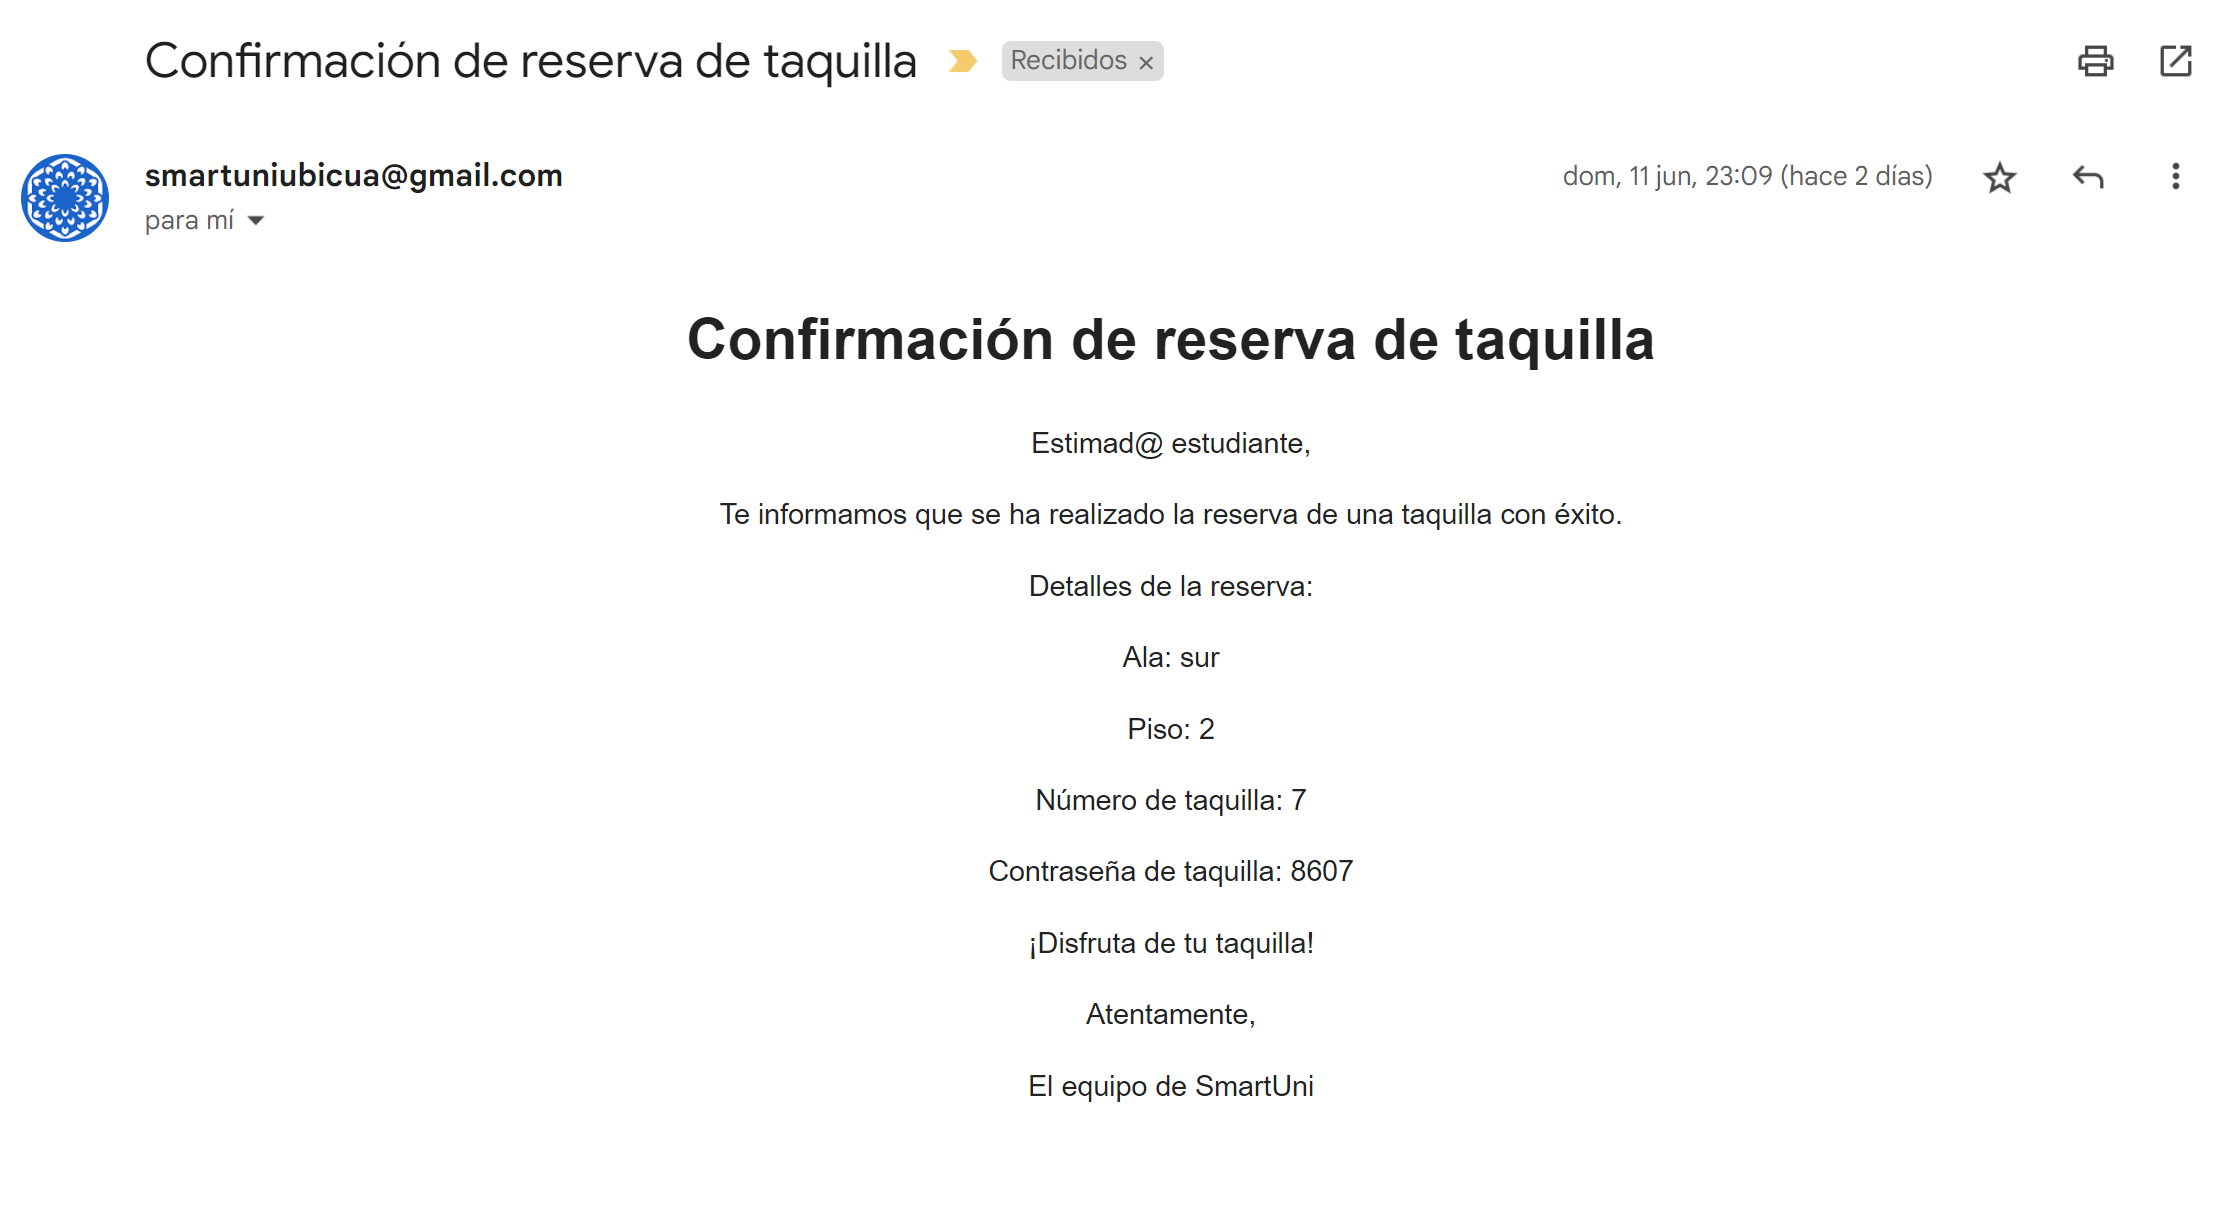
\includegraphics[width=0.8\linewidth]{imagenes//emails/email_confirm_taquilla.png}
        \caption{Email con los datos de la reserva}
        \label{fig:enter-label}
    \end{figure}
    \item \textbf{Email de confirmación de pedido:}
    El alumno recibirá un mensaje en su bandeja de entrada tras haber realizado un pedido de la cafetería. En este, el usuario podrá revisar los datos de su pedido.
    \begin{figure}[H]
        \centering
        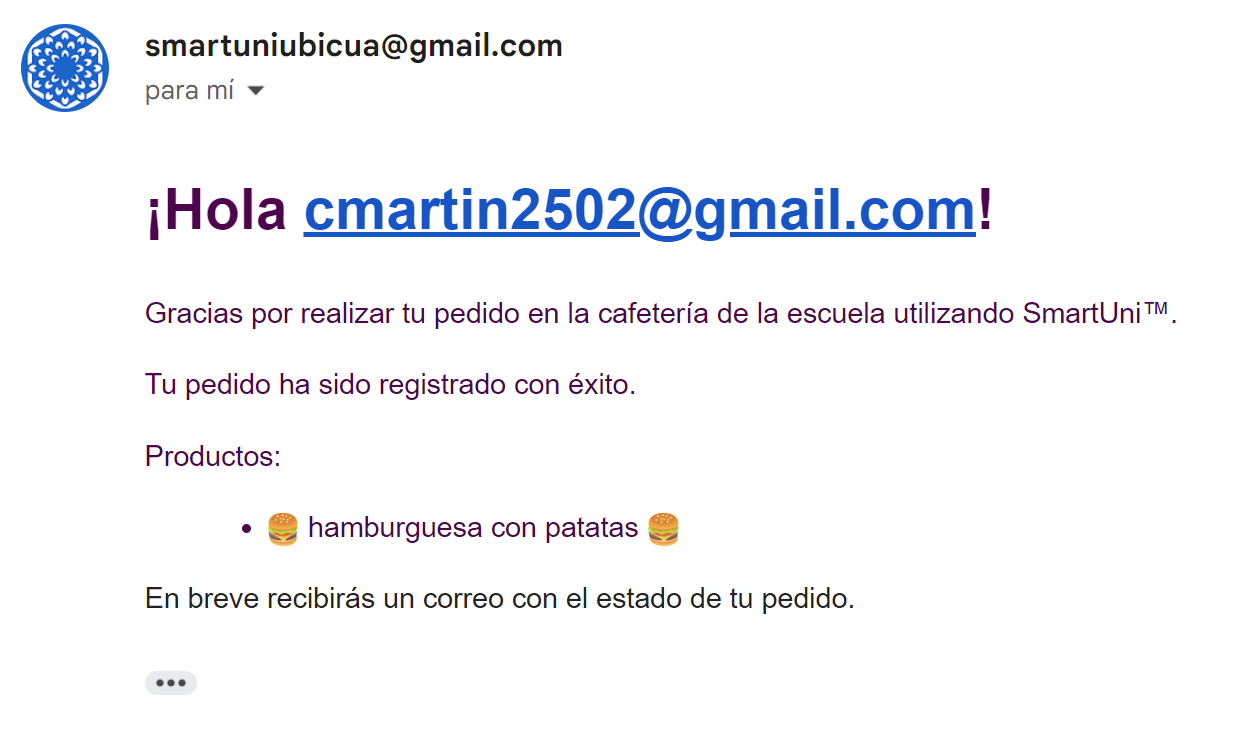
\includegraphics[width=0.8\linewidth]{imagenes//emails/email_confirm_pedido.png}
        \caption{Email con los datos del pedido}
        \label{fig:enter-label}
    \end{figure}
    \item \textbf{Email de aviso de de disponibilidad de pedido:}
    En el momento en el que la cafetería termine de preparar un pedido y esté listo para su recogida, el alumno será avisado mediante un correo electrónico como el siguiente:
    \begin{figure}[H]
        \centering
        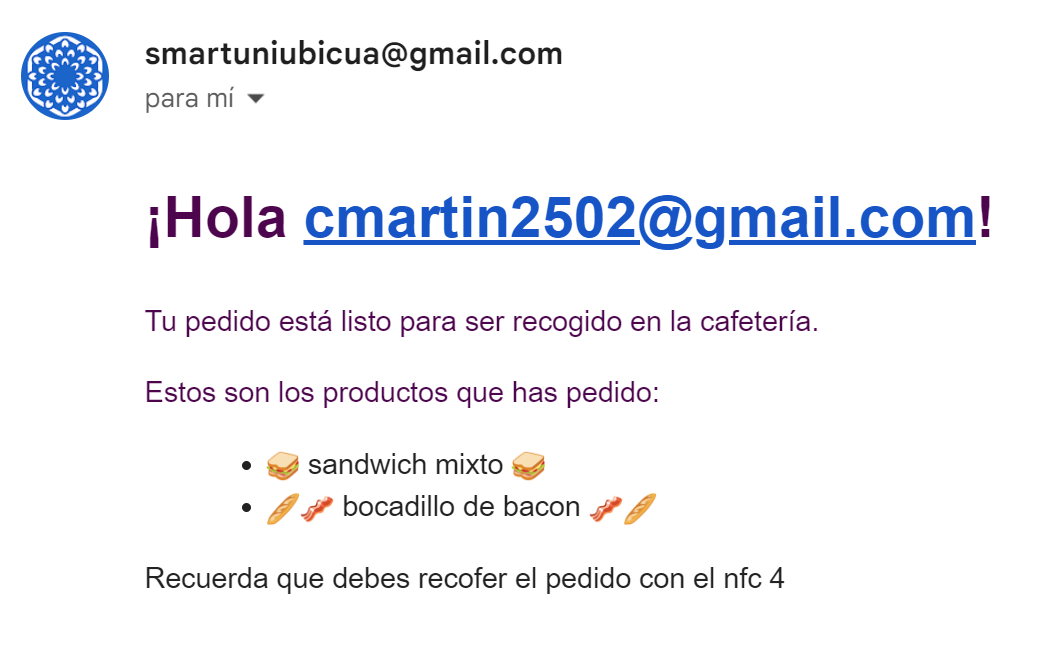
\includegraphics[width=0.8\linewidth]{imagenes//emails/email_pedido_listo.png}
        \caption{Email avisando de la disponibilidad}
        \label{fig:enter-label}
    \end{figure}
\end{itemize}


\section{Endpoints}
Como se ha mencionado en apartados anteriores, los \textit{endpoints} han sido organizados de manera categórica dentro de diversos ficheros. Nuestros endpoints se han distinguido en las siguientes categorías
\begin{itemize}
    \item \textbf{Sesión}\\
    Dentro del fichero \textit{sesion.py} se pueden encontrar los \textit{endpoints} relacionados con el inicio de sesión y registro de usuarios en la plataforma. Un usuario al ser registrado, recibe un email de bienvenida.
    \item \textbf{Páginas HTML}\\
    Dentro del fichero \textit{paginasHTML.py} se alojan todos los endpoints que retornan las páginas \textit{HTML} junto con su hoja de estilos \textit{CSS} y código \textit{JavaScript} asociado. Es una manera simple y organizada de conectar el \textit{FrontEnd} al \textit{BackEnd}.
    \item \textbf{Taquillas}\\
    En el fichero \textit{taquillas.py} podemos encontrar todos los nodos terminales relacionados con la gestión de taquillas.
    Entre dichos endpoints encontramos:
    \begin{itemize}
        \item \textcolor{ForestGreen}{\texttt{GET}} \textit{Lista Taquillas}\\
        Retorna un listado de todas las taquillas del sistema.\\
        Permite realizar un filtrado según el ala, el piso, el pasillo y la ocupación de la taquilla.
        Localizado en: \texttt{(host)/taquillas}
        \item \textcolor{ForestGreen}{\texttt{GET}} \textit{Detalle taquilla}\\
        Retorna la información completa y detallada de una taquilla en específico.\\
        Para ello recibe como argumento el id de la taquilla deseada como path parameter.\\
        Localizado en: \texttt{(host)/taquillas/\{id\_taquilla\}}
        \item \textcolor{YellowOrange}{\texttt{POST}} \textit{Insertar taquilla}\\
        Permite insertar una nueva taquilla en el sistema con la información que se envíe en el body de la solicitud.
        \\Localizado en: \texttt{(host)/taquillas}
        \\Ejemplo de cuerpo de la solicitud:
        \begin{verbatim}
            {
                "ala": "este",
                "pasillo": 2,
                "piso": 2
            }
        \end{verbatim}
        \item \textcolor{SkyBlue}{\texttt{PUT}} \textit{Reservar taquilla}\\
        Este endpoint permite reservar una taquilla a partir de una taquilla y un alumno y genera una contraseña.\\
        Recibe como parámetro el \texttt{id\_taquilla} de la taquilla deseada y la información del alumno en el cuerpo de la solicitud.\\
        Localizado en: \texttt{(host)/taquillas/reservar/\{id\_taquilla\}}\\
        Ejemplo de cuerpo de la solicitud:
        \begin{verbatim}
        {
          "id_alumno": 3
        }
        \end{verbatim}
        
        \item \textcolor{SkyBlue}{\texttt{PUT}} \textit{Cancelar taquilla}\\
        Este endpoint cancela la reserva o la asignación de una taquilla a un alumno.\\
        Recibe como parámetros el \texttt{id\_taquilla} y el \texttt{id\_alumno} de la taquilla y el alumno respectivamente.\\
        Localizado en: \texttt{(host)/taquillas/cancelar/\{id\_taquilla\}/\{id\_alumno\}}
                \\Ejemplo de cuerpo de la solicitud:
        \begin{verbatim}
        {
          "id_alumno": 7
        }
        \end{verbatim}

        \item \textcolor{ForestGreen}{\texttt{GET}} \textit{Obtener taquilla reservada}\\
        Este endpoint devuelve el ID de la taquilla reservada por un alumno específico.\\
        Recibe como parámetro el \texttt{id\_alumno} del alumno.\\
        Localizado en: \texttt{(host)/taquilla/Alumno/\{id\_alumno\}}
        \item \textcolor{YellowOrange}{\texttt{POST}} \textit{Abrir taquilla}\\
        Este endpoint permite abrir una taquilla a partir de su ID y una contraseña.\\
        Recibe como parámetro el \texttt{id\_taquilla} de la taquilla deseada y la contraseña en el cuerpo de la solicitud.\\
        Localizado en: \texttt{(host)/taquillas/\{id\_taquilla\}}\\
        Ejemplo de cuerpo de la solicitud:
        \begin{verbatim}
        {
          "password": "contraseña"
        }
        \end{verbatim}
        
    \end{itemize}
    \item \textbf{Aulas}\\
    Todos los endpoints relacionados con la gestión de las aulas se pueden encontrar en \textit{aulas.py}. Entre dichos endpoints encontramos:
    \begin{itemize}
        \item \textcolor{ForestGreen}{\texttt{GET}} \textit{Lista Aulas}\\
        Retorna un listado de todas las aulas de la Escuela Politécnica Superior. Permite también realizar una búsqueda filtrada según el piso del aula, su tipo (Laboratorio o Aula de teoría), ala (Norte, Sur, Este y Oeste)... Dicho filtro se realiza a partir de los query params recibidos.\\
        Localizado en: \texttt{(host)/aulas}
    
        \item \textcolor{ForestGreen}{\texttt{GET}} \textit{Info aula}\\
        Retorna la información completa y detallada de un aula en concreto.\\
        Para ello recibe como argumento el id del aula deseada como path parameter.\\
        Localizado en: \texttt{(host)/aulas/\{id\_aula\}}
        
        \item \textcolor{YellowOrange}{\texttt{POST}} \textit{Insertar aula}\\
        Permite insertar una nueva aula en el sistema con la información que se envíe en el body de la solicitud.\\
        Localizado en: \texttt{(host)/aulas}
        \\Ejemplo de cuerpo de la solicitud:
        \begin{verbatim}
        {
            "temperatura": 23,
            "luminosidad": 40,
            "laboratorio": true,
            "planta": "2",
            "ala": "Sur",
            "num_ala": 3
        }
        \end{verbatim}
        
        \item \textcolor{SkyBlue}{\texttt{PUT}} \textit{Actualizar aula}\\
        Permite actualizar los valores de un aula concreta del sistema con la información que se envíe en el body de la solicitud. Este endpoint es utilizado por parte del Arduino para actualizar valores como la temperatura en tiempo real.\\
        Localizado en: \texttt{(host)/aulas/\{id\_aula\}}
        \\Ejemplo de cuerpo de la solicitud:
        \begin{verbatim}
        {
            "temperatura": 23,
            "luminosidad": 40,
            "laboratorio": true,
            "planta": "2",
            "ala": "Sur",
            "num_ala": 3
        }
        \end{verbatim}
        
        \item \textcolor{ForestGreen}{\texttt{GET}} \textit{Asignaturas de aula}\\
        Obtiene las asignaturas que se imparten en un aula específica.\\
        Recibe como parámetro el \texttt{id\_aula} del aula deseada.\\
        Localizado en: \texttt{(host)/aulas/asignaturas/\{id\_aula\}}
    
        \item \textcolor{ForestGreen}{\texttt{GET}} \textit{Disponibilidad de aula}\\
        Se utiliza para saber si un aula está en uso en los próximos minutos. Principalmente usado por el Arduino para saber si debe encender o apagar el climatizador.\\
        Recibe como parámetro el \texttt{id\_aula} del aula deseada.\\
        Localizado en: \texttt{(host)/aulas/disponibilidad/\{id\_aula\}}
    
        \item \textcolor{ForestGreen}{\texttt{GET}} \textit{Horario de aula}\\
        Obtiene el horario de un aula en específico.\\
        Recibe como parámetro el \texttt{id\_horario} del horario deseado.\\
        Localizado en: \texttt{(host)/aulas/horarios/\{id\_horario\}}
    
        \item \textcolor{YellowOrange}{\texttt{POST}} \textit{Insertar horario}\\
        Permite insertar un nuevo horario de clase en el sistema con la información que se envíe en el body de la solicitud.\\
        Localizado en: \texttt{(host)/aulas/horarios}
            \\Ejemplo de cuerpo de la solicitud:
        \begin{verbatim}
        {
             "dia": "2023/06/02",
             "hora_inicio": "8:00",
             "hora_fin": "10:00",
             "id_asignatura_asignatura": 3,
             "id_aula_aula": 1
         }
        \end{verbatim}
        
        \item \textcolor{ForestGreen}{\texttt{GET}} \textit{Climatizar aula}\\
        Se encarga de decir si es el momento adecuado para climatizar un aula o no. Esto se realiza de manera inteligente, pues basándose en los datos de las climatizaciones más recientes de ese aula, se estima el tiempo que puede tardar un aula en obtener las condiciones ideales. Teniendo en cuenta ese tiempo y sabiendo cuándo empezará la próxima clase, se devolverá true (para señalar que se debe climatizar el aula) o un error 400 (para señalizar lo opuesto). Realizando gestiones de temperatura de esta manera se reduce en gran medida el consumo de energía para este proceso y se sigue asegurando una temperatura ideal.\\
        Localizado en: \texttt{(host)/aulas/\{id\_aula\}/climatizar}

        \item \textcolor{YellowOrange}{\texttt{POST}} \textit{Insertar histórico}\\
        Tras haber finalizado el proceso de climatización de un aula, el Arduino llamará a este endpoint para anotar la temperatura a la que estaba el aula antes de intervenir, y anotará también el tiempo empleado en adecuar la temperatura. Estos datos serán útiles de cara a mejorar las estimaciones inteligentes explicadas en el endpoint anterior.\\
        Localizado en: \texttt{(host)/aulas/historico}
            \\Ejemplo de cuerpo de la solicitud:
        \begin{verbatim}
        {
          "id_aula_aula":1,
          "temperatura_previa":21,
          "tiempo_calentar":12
        }
        \end{verbatim}
    \end{itemize}

    \item \textbf{Cafetería}\\
    La implementación de la cafetería se ha distribuido en tres ficheros diferentes:
    \begin{itemize}
        \item \texttt{productos.py}:
        Aquí se encuentra toda la lógica relacionada con los productos de la carta de la cafetería. Cuenta simplemente con dos endpoints:
        \begin{itemize}
            \item \textcolor{ForestGreen}{\texttt{GET}} \textit{Productos de la cafetería}\\
            Obtiene todos los productos que están disponibles en la cafetería. Puede filtrar los productos según su nombre, dado un parámetro de búsqueda. Si no se especifica un parámetro de búsqueda, se obtienen todos los productos.\\
            Localizado en: \texttt{(host)/cafeteria/productos}
            \item \textcolor{ForestGreen}{\texttt{GET}} \textit{Detalle de producto}\\
            Detalla toda la información de un producto en específico de la cafetería.\\
            Recibe como parámetro el \texttt{id\_producto} del producto deseado.\\
            Localizado en: \texttt{(host)/cafeteria/productos/\{id\_producto\}}
        \end{itemize}

    
        \item \texttt{pedidos.py}
        Aquí se encuentra toda la lógica relacionada con los pedidos de la cafetería. Cuenta con los siguientes endpoints:
        \begin{itemize}

            \item \textcolor{ForestGreen}{\texttt{GET}} \textit{Pedidos de la cafetería}\\
            Obtiene todos los pedidos que se han realizado en la cafetería.\\
            Localizado en: \texttt{(host)/cafeteria/pedidos}
            \item \textcolor{ForestGreen}{\texttt{GET}} \textit{Detalle de pedido}\\
            Detalla toda la información de un pedido en específico de la cafetería.\\
            Recibe como parámetro el \texttt{id\_pedido} del pedido deseado.\\
            Localizado en: \texttt{(host)/cafeteria/pedidos/\{id\_pedido\}}
            \item \textcolor{YellowOrange}{\texttt{POST}} \textit{Insertar pedido}\\
            Este endpoint permite al usuario realizar un pedido.\\
            Localizado en: \texttt{(host)/cafeteria/pedidos}
            \\Ejemplo de cuerpo de la solicitud:
            \begin{verbatim}
            {
                "id_alumno" : 3,
                "productos" : [1,2,3]
            }
            \end{verbatim}

            \item \textcolor{SkyBlue}{\texttt{PUT}} \textit{Actualizar pedido}\\
            Este endpoint permite a la cafetería actualizar un pedido.\\
            Se puede actualizar el estado del pedido.\\
            Localizado en: \texttt{(host)/cafeteria/pedidos/\{id\_pedido\}}
            \\Ejemplo de cuerpo de la solicitud:
            \begin{verbatim}
            
            {
                "id_alumno" : 5,
                "estado" : 2
            }
            \end{verbatim}
            \item \textcolor{ForestGreen}{\texttt{GET}} \textit{Pedido estrella}\\
            Detalla la descripción del producto más pedido.\\
            Recibe como parámetro el \texttt{id\_alumno} del alumno del que se quiere obtener el pedido estrella.\\
            En caso de no especificar el parámetro, se obtendrá el pedido estrella de todos los alumnos.\\
            Se ha implementado de esta manera para poder obtener el pedido estrella de un alumno en concreto, o de todos los alumnos en general.\\
            Localizado en: \texttt{(host)/cafeteria/pedidos/estrella}

        \end{itemize}

        \item \texttt{NFC.py}: Los NFC cuentan con varios endpoints a destacar. Originalmente iban a tener una funcionalidad que iba a ir más allá de limitarse únicamente a la verificación de pedidos de la cafetería. Desgraciadamente se tuvo que descartar esa idea. Los endpoints a destacar son:
        \begin{itemize}
            \item \textcolor{ForestGreen}{\texttt{GET}} \textit{Listar NFCs}\\
            Obtiene un listado con todos los NFCs que están registrados en el sistema.\\
            Localizado en: \texttt{(host)/nfc}
            \item \textcolor{ForestGreen}{\texttt{GET}} \textit{Detalle de NFC}\\
            Detalla toda la información de un NFC en específico.\\
            Recibe como parámetro de ruta el \texttt{id\_nfc} del NFC deseado.\\
            Localizado en: \texttt{(host)/nfc/\{id\_nfc\}}
            \item \textcolor{YellowOrange}{\texttt{POST}} \textit{Insertar NFC}\\
            Este endpoint permite registrar un nuevo NFC en el sistema.\\
            En concreto se necesitará enviar el número de serie del NFC.\\
            El endpoint verificará que el número de serie no esté ya registrado en el sistema.\\
            Localizado en: \texttt{(host)/nfc}
            \\Ejemplo de cuerpo de la solicitud:
            \begin{verbatim}
            {
                "num_serie": "cr:23:e5:s2"
            }
            \end{verbatim}
            \item \textcolor{SkyBlue}{\texttt{PUT}} \textit{Actualizar NFC}\\
            Este endpoint permite actualizar un NFC en el sistema.\\
            De manera análoga al endpoint de inserción, se necesitará enviar el número de serie del NFC.\\
            El endpoint verificará que el número de serie no esté ya registrado en el sistema.\\
            Localizado en: \texttt{(host)/nfc/\{id\_nfc\}}
            \\Ejemplo de cuerpo de la solicitud:
            \begin{verbatim}
            {
                "num_serie": "cq:15:93:vv"
            }
            \end{verbatim}
        % /cafeteria/pedidos/nfc/:idPedido actualizar pedido con nfc
            \item \textcolor{SkyBlue}{\texttt{PUT}} \textit{Actualizar pedido con NFC}\\
            Este endpoint permite actualizar un pedido de la cafetería con un NFC.\\
            Será utilizado en la verificación de la recogida de un pedido, para que el alumno pueda recoger su pedido una vez esté preparado.\\
            También lo usaría la cafetería para marcar como finalizado un pedido, pudiendo así desvincular el NFC del pedido.\\
            Localizado en: \texttt{(host)/cafeteria/pedidos/nfc/\{id\_pedido\}}
            \\Ejemplo de cuerpo de la solicitud:
            \begin{verbatim}
            {
                "num_serie": "04:ef:8e:56:70:00:00",
                "id_alumno" : 3,
                "estado" : 3
            }
            \end{verbatim}
        \end{itemize}
    \end{itemize}
    
\end{itemize}

\section{Documentación de la API}
Aprovechando también las características que nos brinda \textit{FastApi} se ha creado una documentación completa e interactiva de la API, alojada en \texttt{(host)/docs}.\\
Esta documentación permite ejecutar cualquiera de los endpoints creados de manera muy intuitiva, algo muy útil para realizar pruebas rápidas si no se quiere pasar por el proceso de configurar \textit{Postman}.
\begin{figure}[H]
    \centering
    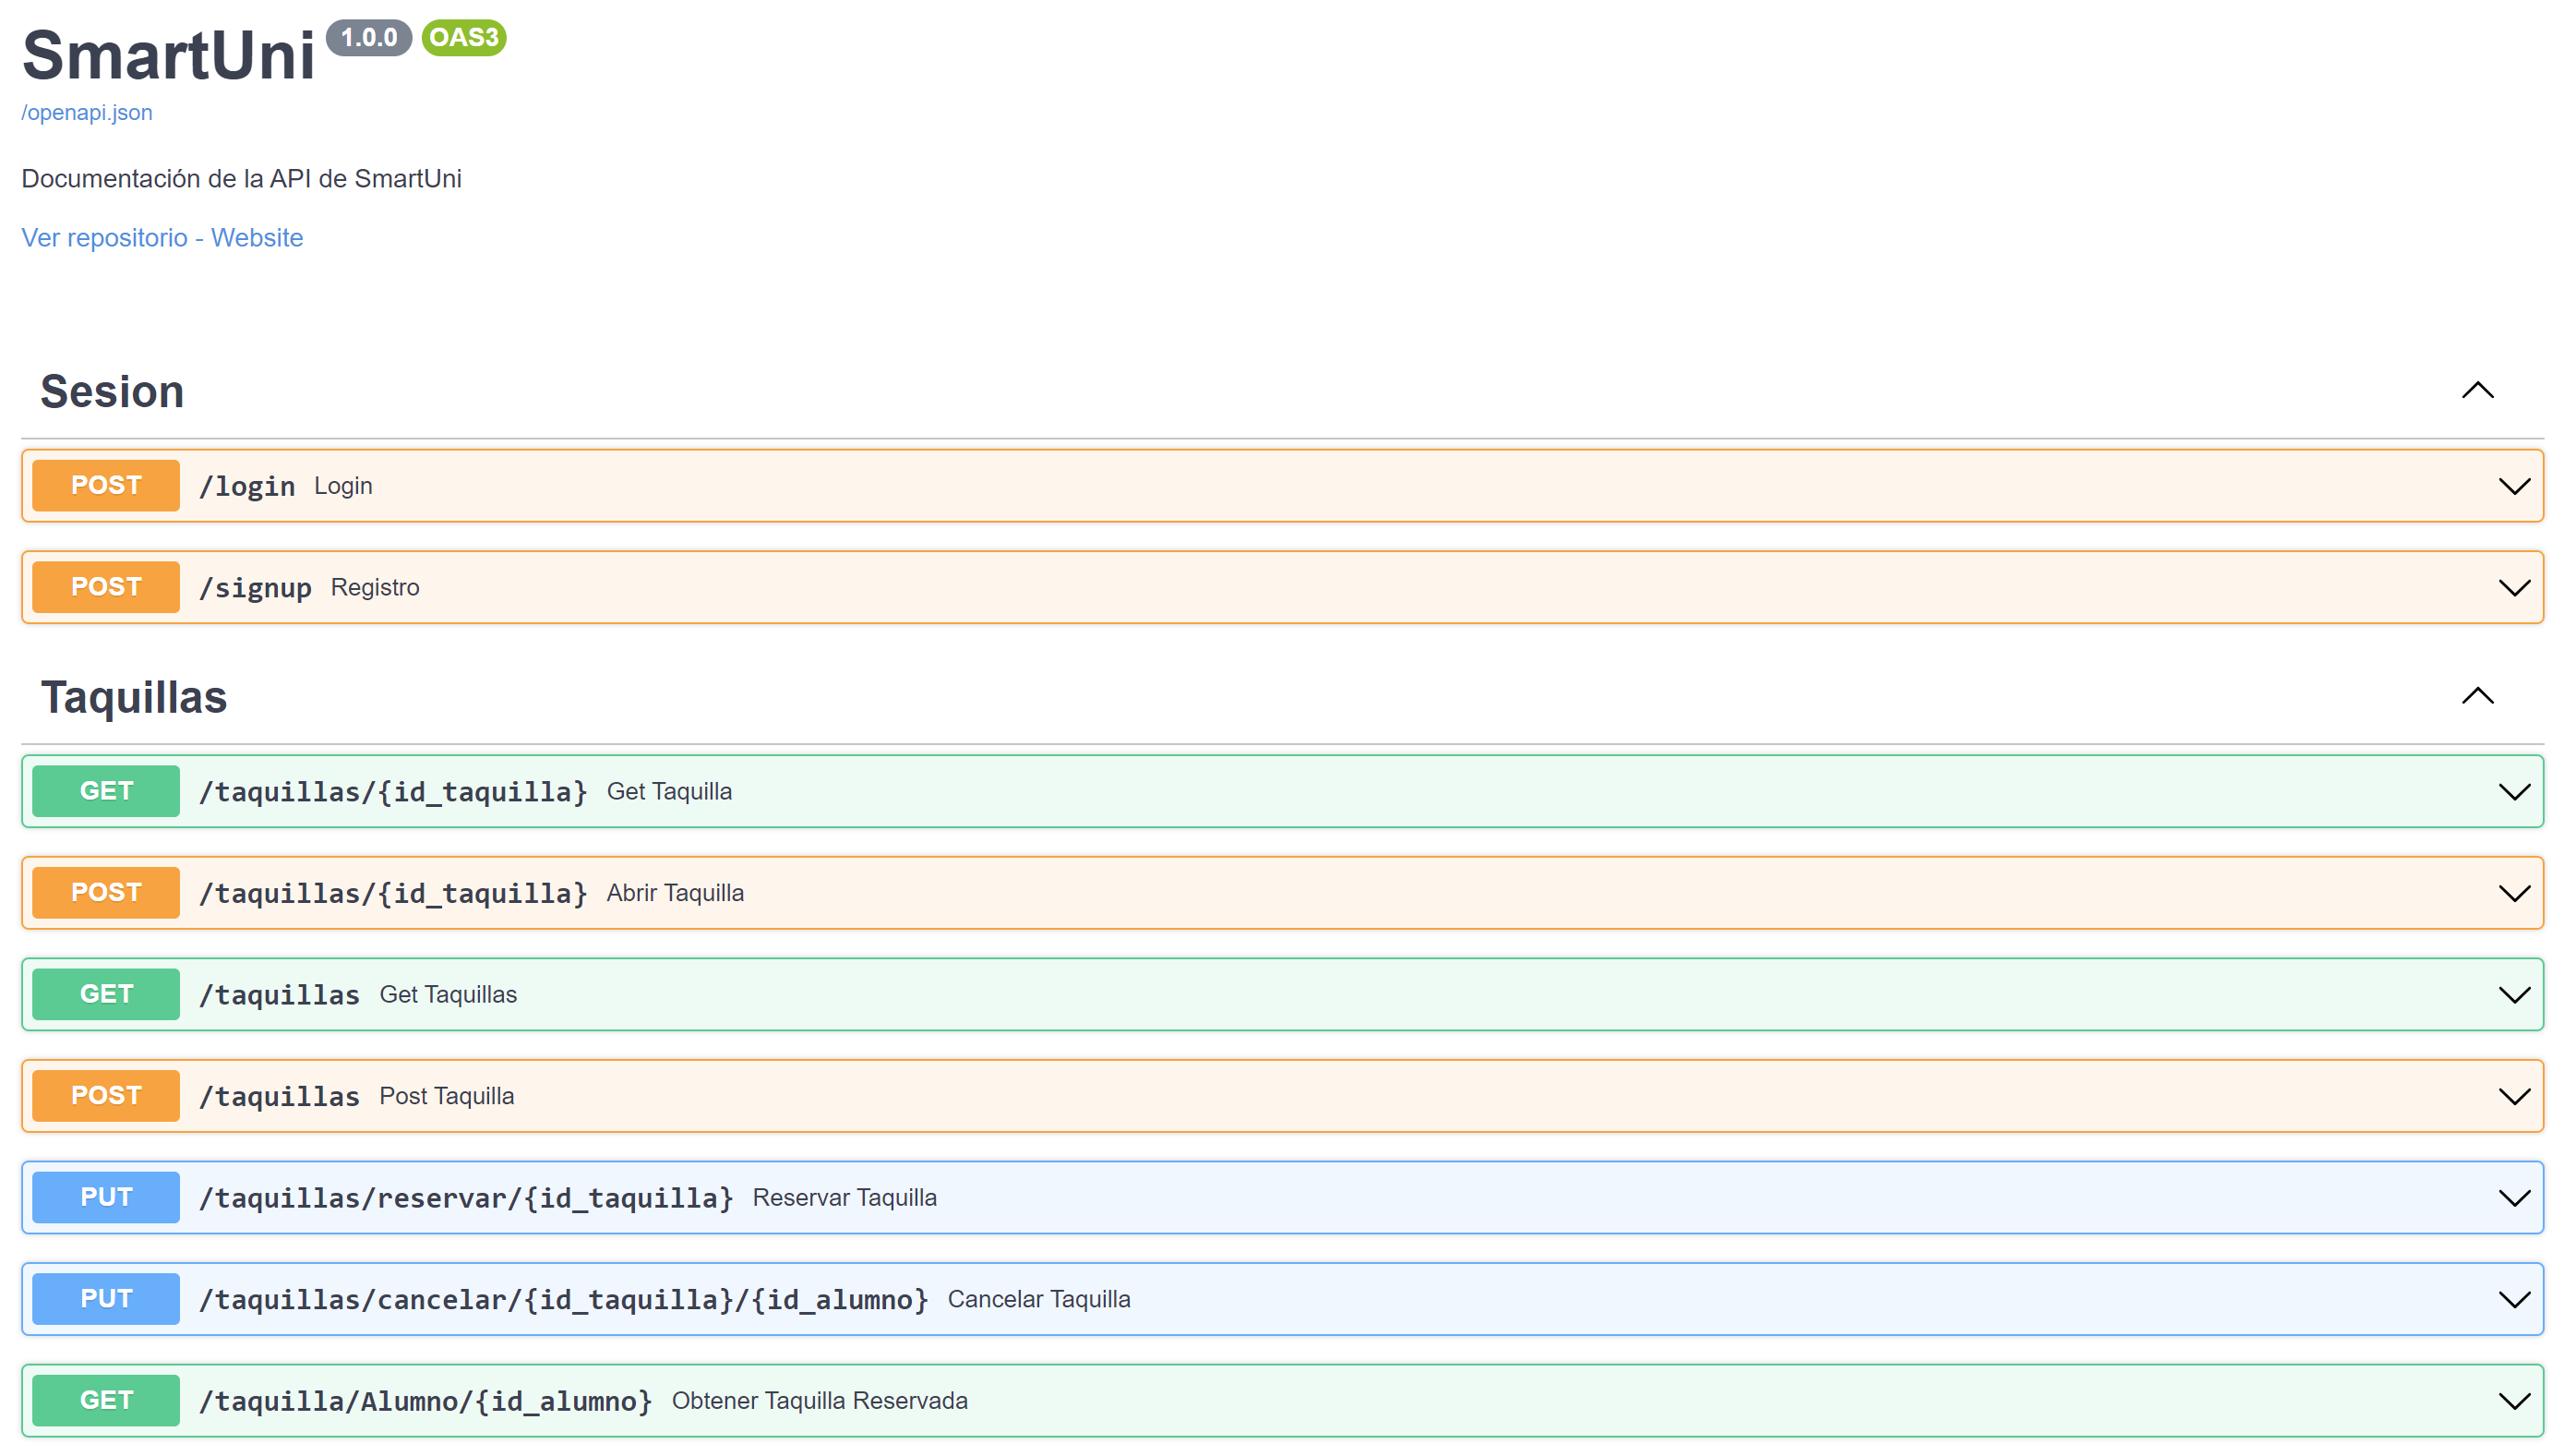
\includegraphics[width=0.75\linewidth]{imagenes//documentacion/captura_documentacion.png}
    \caption{Documentación de la API}
    \label{fig:enter-label}
\end{figure}
A continuación se muestra un ejemplo de testeo del endpoint 
\texttt{/taquillas/\{id\_taquilla\}} utilizando esta documentación:
\begin{figure}[H]
    \centering
    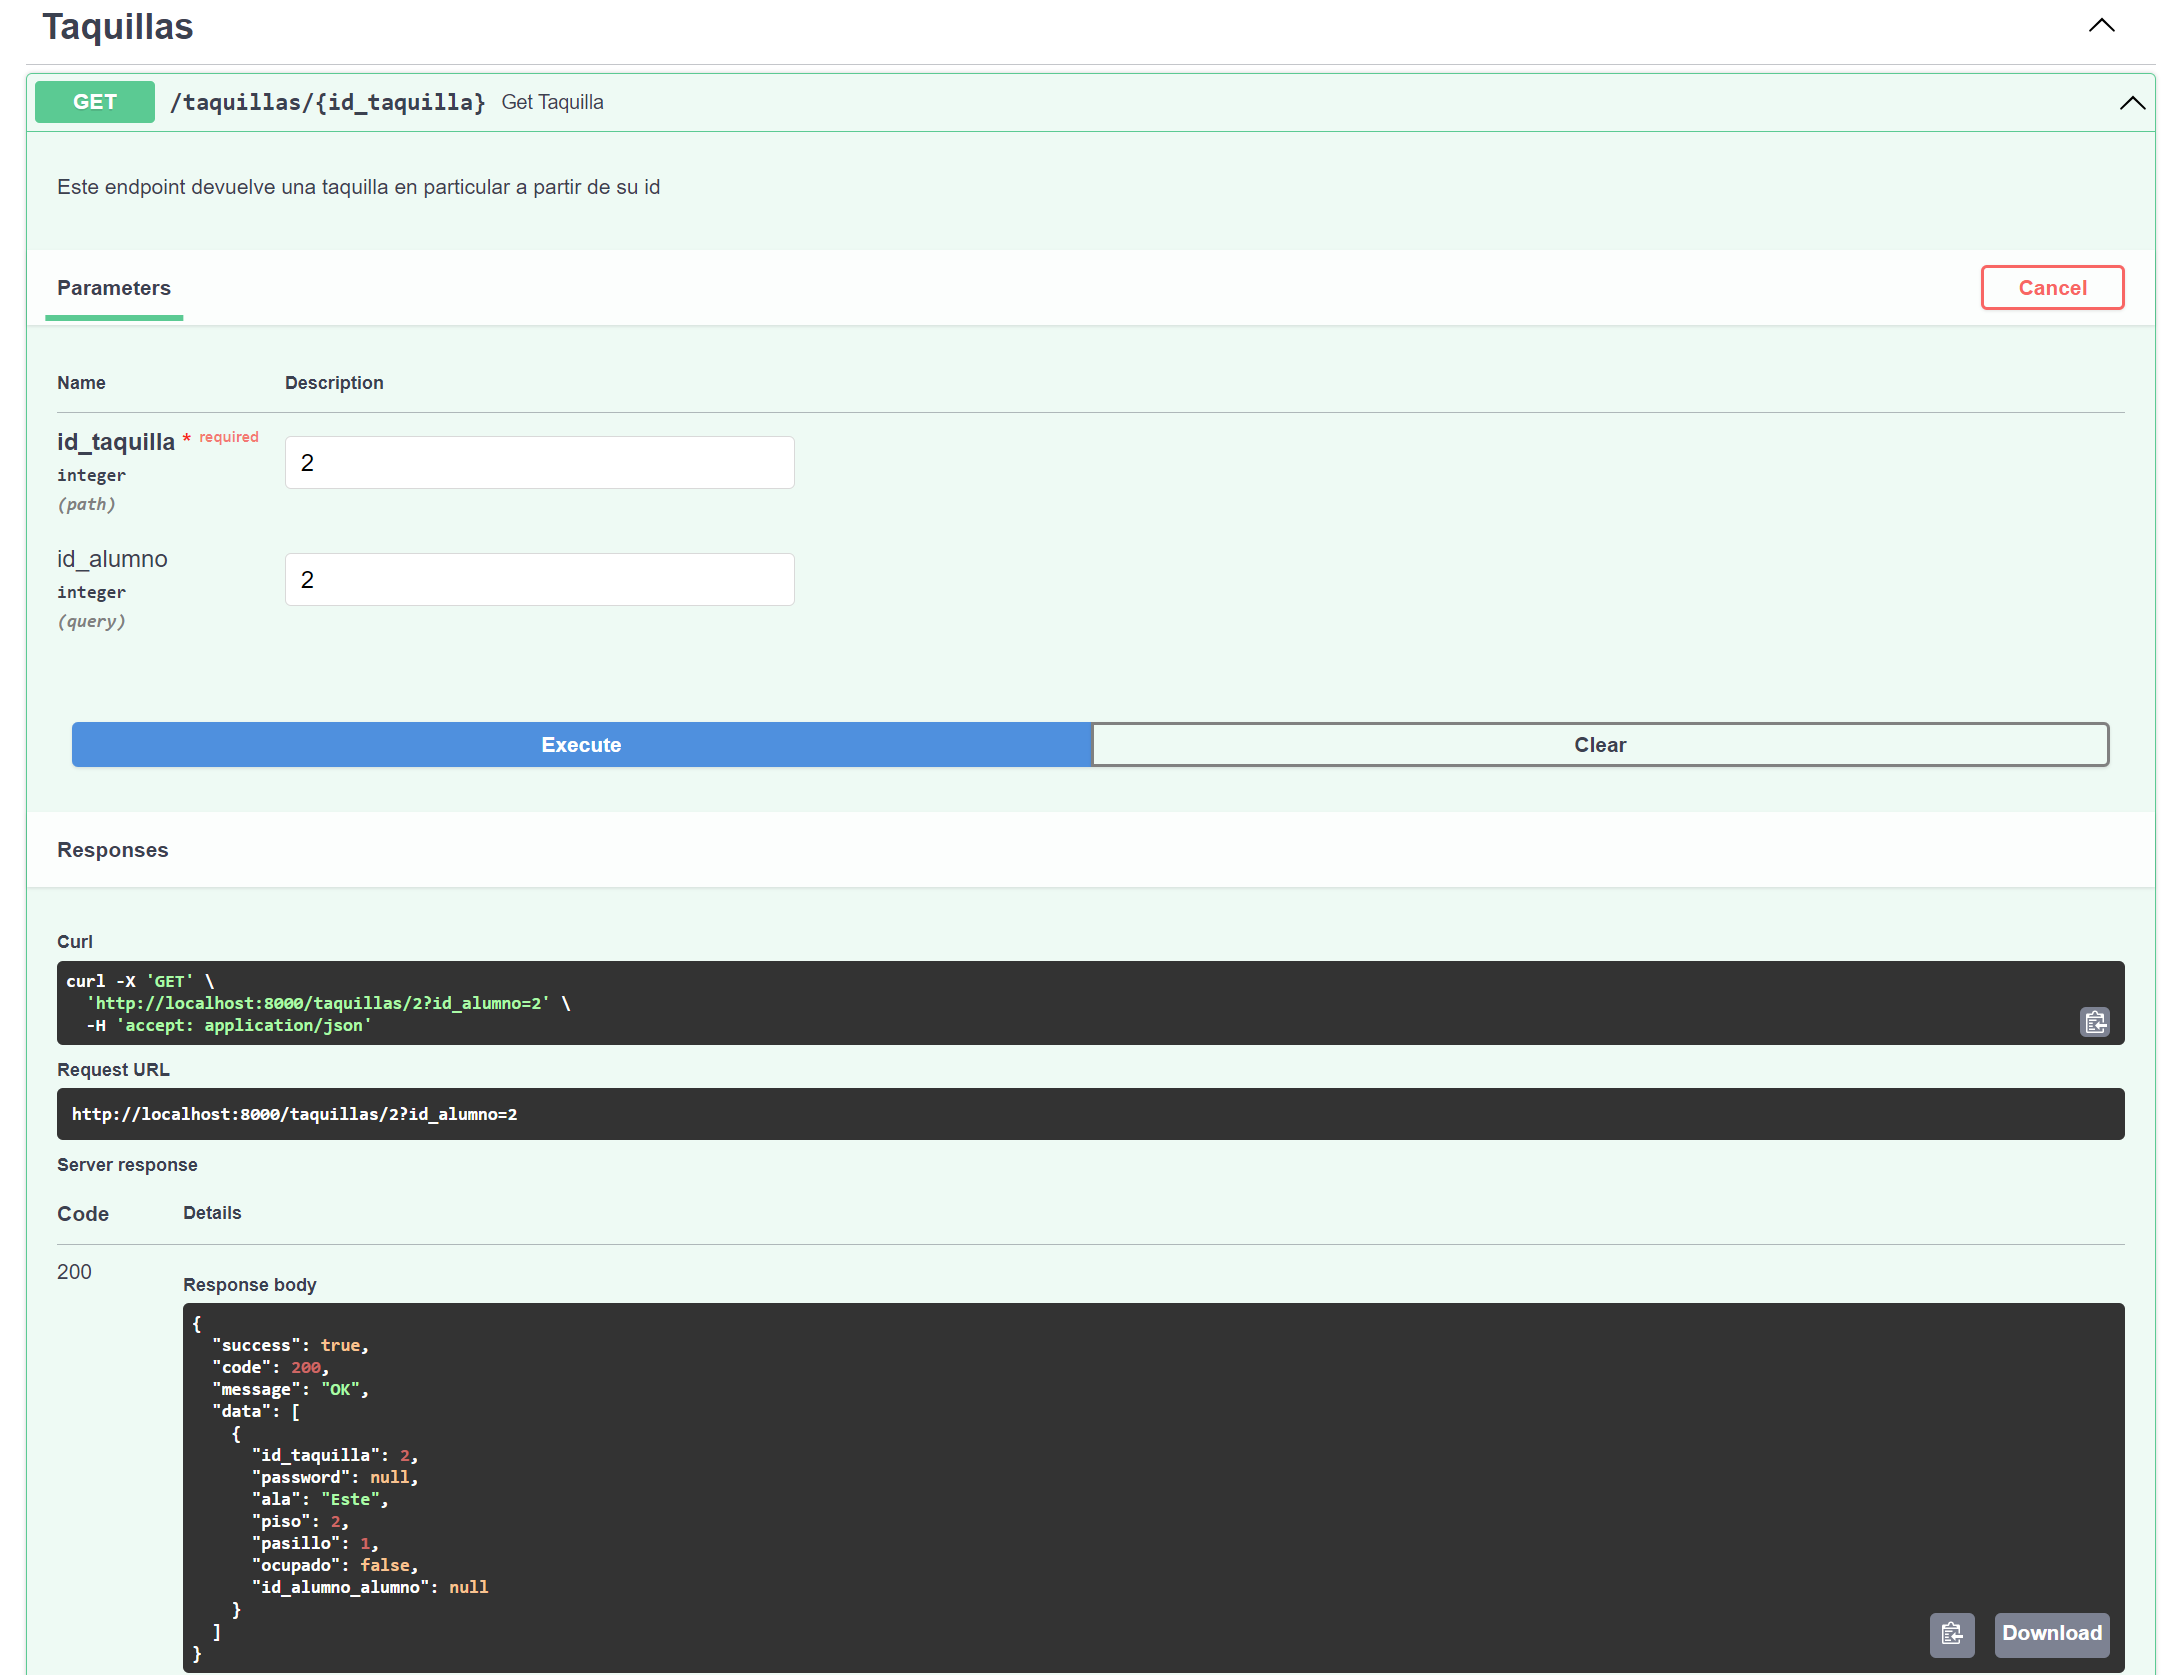
\includegraphics[width=1\linewidth]{imagenes//documentacion/documentacion_testeo_endpoint.png}
    \caption{Testeo de endpoint desde la documentación}
    \label{fig:enter-label}
\end{figure}

\chapter{Diseño e implementación del front-end}
En esta sección, se detalla el diseño y la implementación del front-end de la aplicación web del proyecto. El front-end se encarga de la interfaz de usuario y la interacción con el usuario. Se utilizan tecnologías como HTML, CSS y JavaScript para crear una experiencia visual agradable y funcional. \\
La implementación del front\textendash end se ha realizado utilizando: HTML para la estructura y el contenido de las páginas, CSS para dar estilo y diseño a los elementos visuales, y JavaScript para la interactividad y la lógica de la aplicación en el lado del cliente.
\\

\section{Estructura HTML}
En esta sección se detallan y explican los diferentes elementos y funcionalidades de los archivos HTML utilizados en la implementación del front-end de la aplicación web SmartUni.
\subsection{Página de Inicio de Sesión}
La página de inicio de sesión (index.html) es la primera pantalla que los usuarios ven al acceder a la plataforma SmartUni. Su objetivo es permitir que los usuarios inicien sesión en sus cuentas existentes o se registren como nuevos usuarios.\\\\
El encabezado\textbf{ \textless head\textgreater} del archivo HTML contiene metadatos esenciales, como la codificación de caracteres, la configuración de la vista en los dispositivos y el título de la página. Además, se vincula el archivo main.css para aplicar estilos personalizados a la página. El ícono de SmartUni también se establece a través del enlace a la imagen favicon.png. El archivo index.js se enlaza al final del encabezado y contiene el código JavaScript específico de esta página.\\\\
En el cuerpo\textbf{ \textless body\textgreater} de la página, se encuentra el contenido principal contenido dentro del elemento principal \textbf{ \textless main\textgreater}.\\
La página muestra el logo de SmartUni utilizando la etiqueta\textbf{ \textless img\textgreater} con la clase 'logo' para aplicar estilos específicos a la imagen.\\
Se presenta un formulario de inicio de sesión dentro de un contenedor div con la clase 'menu'\textbf{ \textless div class="menu"\textgreater}. El formulario\textbf{ \textless form id="loginForm"\textgreater} solicita al usuario su dirección de correo electrónico y contraseña para autenticarse en la plataforma. Cuando el usuario envía el formulario haciendo clic en el botón 'INICIAR SESIÓN', se ejecuta la función iniciarSesion() definida en el archivo index.js. Los campos de entrada de texto se definen con los elementos\textbf{ \textless input\textgreater}, donde se especifica el tipo de entrada (text o password), y se les asigna un id para identificarlos en el código JavaScript.\\\\
Si se produce algún error durante el proceso de inicio de sesión, se muestra un mensaje de error utilizando el elemento h3 con la clase 'errorMsg'\textbf{ \textless h3 class=''errorMsg''\textgreater}. Este mensaje se oculta inicialmente estableciendo su estilo de visualización en "none", y el código JavaScript puede mostrarlo si es necesario.
El atributo \textbf{id=''errorInicioSesion''} se utiliza para identificar este elemento en el código JavaScript y aplicar cambios en su estilo.\\
Se proporciona un enlace al formulario de registro para los usuarios que aún no tienen una cuenta. Al hacer clic en el enlace 'REGISTRATE', los usuarios serán redirigidos a la página de registro, ya que el elemento \textbf{\textless a\textgreater} se utiliza como un enlace para redirigir al usuario a la página de registro.
\\\\
La página de inicio de sesión de SmartUni presenta una interfaz sencilla y amigable que permite a los usuarios autenticarse en la plataforma utilizando su correo electrónico y contraseña, ofreciendo la opción de registrarse para los nuevos usuarios.

\subsection{Página de Registro}
El archivo ''registrarse.html'' es la página de registro de SmartUni. En esta página se puede encontrar un formulario para crear una nueva cuenta de usuario (alumno).
A continuación, se muestra una descripción de la estructura principal y la función de este archivo.\\
Las etiquetas estándar para caracteres, título de página y vinculación de archivos están contenidas en el encabezado \textbf{(head)}. También se incluye un enlace al icono de la aplicación. \\
En el cuerpo \textbf{(body)} del archivo, se encuentra el contenido principal contenido dentro del elemento principal \textbf{(main)}.  El logotipo se muestra en la etiqueta img con la clase ''logotipo'' en la página. \\\\
Dentro del \textbf{contenedor div con la clase "menu"}, está el título ''REGISTER'' representado por la etiqueta h1. ''Correo electrónico'', ''Contraseña'' y ''Repetir contraseña'' son los campos de entrada para el formulario de registro. Los campos están representados por las etiquetas de entrada. \\\\
Hay una acción en línea definida como \textbf{''javascript:registrarse(parámetros)''} en el formulario. Los valores ingresados en los campos de entrada se usarán para a una función en el archivo ''registrarse.js''. 
Si hay algún error durante el proceso de registro, se mostrará un mensaje de error oculto después de completar el formulario. 
\\
El enlace a la página de inicio de sesión para los usuarios que ya tienen una cuenta se muestra con este elemento. Este enlace redirige al usuario a la página principal utilizando la propiedad href.
\\
El\textbf{ script ''registrarse.js''} contiene la implementación una función que se invoca al enviar el formulario. La función se encarga de validar los campos de entrada y realizar una solicitud de registro al servidor a través de la API.
\\
Se proporciona un formulario en la página de registro para crear una nueva cuenta. Antes de que se envíe una solicitud a un servidor, se verifican los campos de entrada.


\subsection{Página de Menú}
Este archivo ''menu.html'' se encarga de mostrar el menú principal de navegación de la aplicación SmartUni. A continuación, se describen los elementos clave de este archivo.
\\\\
El encabezado \textbf{(head) }del archivo HTML es similar al del archivo "index.html", ya que se utiliza el mismo conjunto de etiquetas para definir la codificación de caracteres, el título de la página y la vinculación de archivos CSS. \\\\
En el cuerpo \textbf{(body)} del archivo, se encuentra el contenido del elemento principal\textbf{ (main)}. En la que se muestra el logo de SmartUni usando la etiqueta img con la clase "logo". Al hacer clic en el logo, los usuarios serán redirigidos a la página principal del menú.
\\
Dentro del contenedor \textbf{div} con la clase "menu", se encuentran los botones que representan las diferentes secciones de la aplicación. Los botones se crean utilizando la etiqueta button con la clase "btn-menu" y un identificador único. En este caso, se presentan los botones ''CLASES", "TAQUILLAS", ''CAFETERÍA'' y ''CERRAR SESIÓN". Cada botón lleva a cabo una acción específica cuando se hace clic en él.
\\\\
Para cada botón del menú, se agrega un evento de escucha (event listener) utilizando JavaScript \textbf{\textless script\textgreater}. Cuando se hace clic en un botón, se ejecuta una función específica que realiza una acción correspondiente, como redirigir al usuario a una página específica de la aplicación.
\begin{itemize}
    \item Para el\textbf{ botón ''CAFETERÍA''}, se agrega un evento de escucha. Cuando se hace clic en el botón, se redirige al usuario a la página de la cafetería (/cafeteria). Esto se logra mediante la modificación de la propiedad "href" de la ventana del navegador.
    
    \item El \textbf{botón ''TAQUILLAS''} también cuenta con un evento de escucha. Al hacer clic en este botón, se ejecuta la función ''obtenerTaquillaReservada()'' que realiza una operación específica relacionada con las taquillas.
    
    \item El \textbf{botón ''CLASES'' }redirige al usuario a la página de las aulas (/aula) al hacer clic en él.
    
    \item El \textbf{botón ''CERRAR SESIÓN'' }tiene un evento de escucha que ejecuta la función ''cerrarSesion()'' cuando se hace clic en él. Esta función realiza la acción de cerrar la sesión del usuario en la aplicación.
\end{itemize}
Esta página html representa el menú principal de navegación de la aplicación SmartUni. Proporciona botones interactivos que permiten a los usuarios acceder a diferentes secciones de la aplicación, como las clases, las taquillas y la cafetería. Además, se incluye un botón para cerrar la sesión del usuario.


\subsection{Página de Aulas}
Dentro de la aplicación SmartUni, se encuentra la página ''aulas.html'', la cual desempeña el papel de mostrar y proporcionar información sobre las aulas disponibles.
\\\\
En el encabezado \textbf{(head)} del archivo HTML, se definen las etiquetas estándar para establecer la codificación de caracteres, el título de la página y la vinculación de archivos CSS y JavaScript. También se incluye un enlace en el ícono de la aplicación.
\\\\
En el cuerpo \textbf{(body)} del archivo, se encuentra el contenido principal, contenido dentro del elemento principal \textbf{(main)}. El inicio de la página muestra el logotipo de SmartUni utilizando la etiqueta ''img'' y la clase ''logo''.
\\
Tenemos el contenedor ''div'' con la \textbf{clase ''menu''}. Aquí se encuentra el título ''AULAS'' en un elemento ''h1''. Además, hay otro contenedor ''div'' con el \textbf{identificador ''aulas''}, que servirá para mostrar la lista de aulas disponibles.
\\\\
La funcionalidad de redirección está implementada a través de un \textbf{script}. Al asignar un evento de escucha al logotipo de SmartUni con el identificador ''logo'', se logra redirigir al usuario a la página principal al hacer clic en el logo. Esto se logra utilizando la función window.location.href y enlazando la página principal con ''/menu''.
\\\\
Además, se agrega un archivo JavaScript externo llamado \textbf{''listarAulas.js''} utilizando el atributo defer. Este archivo contiene la lógica necesaria para obtener la lista de aulas desde el servidor mediante una API y mostrarla en el contenedor ''div'' con el identificador ''aulas''.
\\\\
Esta página html es responsable de mostrar la información sobre las aulas disponibles. Además, utiliza el logotipo de SmartUni para redirigir al usuario a la página principal. El archivo JavaScript ''listarAulas.js'' se encarga de obtener y mostrar la lista de aulas desde el servidor mediante una API.
 
 \subsection{Página de Detalle de Aula}
Explicaremos la estructura y la funcionalidad de la página ''detalle\_aula.html'' representa la página de detalle de aula en la aplicación SmartUni. Esta página muestra información detallada sobre un aula específica.
\\\\
Con respecto al encabezado \textbf{(head)} como en las páginas, explicadas anteriormente, se sigue un estilo similar, de manera que se usen etiquetas estándar para los estilo de la página, tales como, los caracteres, títulos, iconos, etc.\\\\
Pasaremos a explicar el cuerpo \textbf{(body)} del archivo, que contiene el elemento principal \textbf{(main)}. Al igual que en las páginas anteriores, se tiene un logo de SmartUni mediante la etiqueta ''img'' con clase ''logo''.\\\\
Siguiendo la estructura de la página, tendremos un contenedor \textbf{div con el identificador "datos"}, que mostrará la información detallada del aula específico.
El siguiente contenedor \textbf{div con la clase "wide-menu menu"} contiene el contenedor div con el identificador ''aulas'', que es el lugar donde se mostrará la lista de aulas. Sin embargo, en este caso, se utiliza para mostrar información detallada sobre un aula específica en lugar de una lista.
\\\\ El \textbf{script}  incluido en el archivo tiene la función de redirigir al usuario a la página principal al hacer clic en el logotipo de SmartUni. Esto se logra mediante la asignación de un evento de escucha al elemento de imagen con el identificador ''logo'' y la utilización de la función window.location.href para redirigir al usuario a la página principal (''/menu'').
\\\\Además, en el scprit se incluye la vinculación de un archivo JavaScript externo llamado \textbf{''detalle\_aula.js''} utilizando el atributo type="text/javascript". Este archivo contiene la lógica para obtener y mostrar la información detallada de un aula específica desde el servidor y mostrarla en el contenedor div con el identificador "datos".
\\\\
La página de detalle de aula muestra información detallada sobre un aula específica en la aplicación SmartUni. El logotipo de SmartUni redirige al usuario a la página principal al hacer clic en él. El archivo JavaScript "detalle\_aula.js" se encarga de obtener y mostrar la información detallada del aula desde el servidor.

\subsection{Página de Taquillas}
La página de taquillas de la aplicación SmartUni está contenida en el archivo ''taquillas.html''. Esta página permite a los usuarios acceder y gestionar las taquillas disponibles. Describiremos la estructura y funcionalidad.
\\\\
Las etiquetas estándar para los caracteres, el título de la página y la vinculación del archivo CSS se encuentran en el encabezado \textbf{ (head)} del archivo HTML.
\\\\
En el cuerpo \textbf{(body)} del archivo, se encuentra el contenido principal contenido dentro del elemento principal \textbf{(main)}. La página comienza mostrando el logotipo de SmartUni utilizando la etiqueta img con la clase "logo".\\\\
Dentro del contenedor \textbf{div} con la clase "menu", se encuentra el título de la página "TAQUILLAS'' representado por el elemento h1.
El contenedor div con el identificador "taquillas", que se utiliza para mostrar la lista de taquillas disponibles. Este contenedor se poblará dinámicamente utilizando JavaScript al cargar la página.
\\\\
El \textbf{script} "listarTaquillas.js" se vincula al final del archivo HTML y se carga de forma diferida (defer). Este script se encarga de realizar una solicitud a la API del servidor para obtener la lista de taquillas y luego renderizarla en el contenedor ''taquillas'' utilizando el DOM (Document Object Model).
\\\\
Por tanto,  la página de taquillas permite a los usuarios acceder y visualizar las taquillas disponibles en la aplicación SmartUni. La lista de taquillas se muestra dinámicamente utilizando JavaScript y se obtiene a través de una solicitud a la API del servidor.

\subsection{Página de Detalle de Taquilla}
Dentro de la aplicación SmartUni, el archivo HTML ''detalle\_taquilla.html'' representa la página dedicada a mostrar información detallada de una taquilla específica. Esta página brinda al usuario la posibilidad de conocer en profundidad los detalles de una taquilla seleccionada. A continuación, se describe la estructura y la funcionalidad principal de la página.
\\\\
En el \textbf{encabezado (head)} del archivo HTML se definen las etiquetas estándar para establecer la codificación de caracteres, el título de la página y la vinculación de archivos CSS.
\\\\
En el \textbf{cuerpo (body)} del archivo se encuentra el contenido principal, contenido dentro del elemento principal (main). Al inicio de la página, se muestra el logotipo de SmartUni utilizando la etiqueta ''img'' con la clase ''logo''.
\\\\
El contenedor ''div'' con el \textbf{identificador ''datos''} se utiliza para mostrar información detallada de la taquilla seleccionada. Este contenedor se llenará de forma dinámica utilizando JavaScript al cargar la página.
\\
Dentro de ''div'' con la clase ''wide-menu menu'', se encuentra el contenedor ''div'' con el \textbf{identificador ''taquillas''}. Este contenedor se utiliza para mostrar información adicional relacionada con la taquilla, como su ubicación y estado.
\\\\
Con el script podemos asignar un \textbf{evento de clic} al logo de SmartUni. Cuando se hace clic en el logotipo, se redirige al usuario a la página principal del menú mediante la propiedad window.location.href.
\\\\
El script externo \textbf{''detalle\_taquilla.js''} se vincula al final del archivo HTML y se carga como un archivo de tipo ''text/javascript''. Este script se encarga de obtener los datos específicos de la taquilla seleccionada mediante una solicitud a la API del servidor. Luego, utiliza el DOM (Document Object Model) para renderizar los datos obtenidos en los contenedores ''datos'' y ''taquillas''.\\\\
Esta página muestra de manera detallada información específica de una taquilla seleccionada. Esta información se obtiene dinámicamente a través de una solicitud a la API del servidor y se presenta en la página utilizando JavaScript y el DOM.

\subsection{Página de Cafetería}
El archivo HTML ''cafeteria.html'' representa la página de la cafetería en la aplicación SmartUni. Esta página permite a los usuarios realizar pedidos y ver sus pedidos realizados. A continuación, se describe la estructura y funcionalidad principal de este archivo.
\\\\
El encabezado \textbf{(head)} del archivo HTML contiene las etiquetas estándar para especificar la codificación de caracteres, el título de la página y la vinculación de archivos CSS y el icono de la aplicación.
\\\\En el cuerpo \textbf{(body)} del archivo, se establece la clase ''cafe'' en el elemento body. Esto permite aplicar estilos específicos para la página de la cafetería utilizando CSS.
\\Dentro del elemento principal \textbf{(main)}, se muestra el logotipo de SmartUni utilizando la etiqueta img con la clase "logo". A continuación, se encuentra el contenedor \textbf{div} con la clase "menu", que contiene el título ''CAFETERÍA'' y dos botones.
    \begin{itemize}
        \item El\textbf{ primer botón} con el identificador \textbf{"pedido-btn"} representa el botón para realizar un pedido. Al hacer clic en este botón, se activa un evento que redirige al usuario a la página de realizar un pedido ("/pedido") utilizando la función window.location.href += '/pedido'.
        
        \item El \textbf{segundo botón }con el identificador \textbf{''mis-pedidos-btn'' }representa el botón para ver los pedidos realizados por el usuario. Al hacer clic en este botón, se activa un evento que redirige al usuario a la página de ver mis pedidos ("/mis\_pedidos") utilizando la función window.location.href += '/mis\_pedidos'.
    \end{itemize}
El \textbf{script } incluido en el archivo tiene tres eventos de escucha:
    \begin{itemize}
        \item El evento de escucha del botón \textbf{''pedido-btn''} que redirige al usuario a la página de realizar un pedido al hacer clic en el botón.
        \item El evento de escucha del logotipo \textbf{"logo"} que redirige al usuario a la página principal (''/menu'') al hacer clic en el logotipo.
        \item El evento de escucha del botón \textbf{''mis-pedidos-btn''} que redirige al usuario a la página de ver mis pedidos al hacer clic en el botón.
    \end{itemize}
Esta página de la cafetería en la aplicación SmartUni permite a los usuarios realizar pedidos y ver sus pedidos ya realizados. Los botones ''pedido\-btn'' y ''mis\-pedidos\-btn'' redirigen a los usuarios a las páginas correspondientes (''/pedido'' y ''/mis\_pedidos'') al hacer clic en ellos.

 \subsection{Página de Realizar Pedido en la Cafetería}
El archivo HTML ''cafeteria\_pedido.html'' representa la página de realizar pedido en la cafetería de la aplicación SmartUni. Esta página permite a los usuarios ver los productos disponibles, filtrar por nombre y confirmar su pedido. A continuación, se describe la estructura y funcionalidad principal de este archivo.
\\\\El encabezado\textbf{ (head) }del archivo HTML contiene las etiquetas estándar para especificar la codificación de caracteres, el título de la página (''Realizar pedido - SmartUni'') y la vinculación de archivos CSS y el icono de la aplicación.
\\\\ En el cuerpo \textbf{(body)} del archivo, se establece la clase ''cafe'' en el elemento body para aplicar estilos específicos para la página de realizar pedido utilizando CSS.\\
Dentro del elemento principal \textbf{(main)}, se muestra el logotipo de SmartUni utilizando la etiqueta img con la clase ''logo''. A continuación, se encuentra el título ''REALIZAR PEDIDO'' representado por la etiqueta h1.\\\\
El contenedor \textbf{div} con la \textbf{clase ''menu''} contiene dos secciones para mostrar productos: ''productoEstrella'' y ''productoAlumno''. Estas secciones representan el producto estrella de la cafetería y los productos recomendados para el usuario, respectivamente. Cada sección se muestra con un título representado por la etiqueta h2.
\\\\ A continuación, hay un contenedor \textbf{div con la clase ''filterDiv''} que contiene un formulario para filtrar los productos por nombre. El formulario tiene un campo de entrada de texto con el id ''input'' donde los usuarios pueden ingresar el nombre del producto que desean filtrar. También hay un botón con la clase ''btn'' y el id ''btn'' que, al hacer clic en él, activa la función ''cargarDatos()'' para cargar los datos filtrados.
\\\\Después del \textbf{formulario de filtrado}, se muestra un botón con el id ''realizar-pedido''. Al hacer clic en este botón, se activa la función ''crearPedido()'' para confirmar el pedido.
\\\\Luego, hay un contenedor \textbf{div con la clase ''wide-menu menu''} que contiene los productos disponibles para seleccionar. El título ''PRODUCTOS'' se muestra utilizando la etiqueta h1, y los productos se cargan en el contenedor div con el id ''productos''. Si los productos aún se están cargando, se muestra el mensaje ''CARGANDO'' utilizando la etiqueta h2.
\\\\
El \textbf{script}  incluido en el archivo tiene un evento de escucha para el logotipo ''logo''. Al hacer clic en el logotipo, se redirige al usuario a la página principal (''/menu'') utilizando la función window.location.href = '/menu'.
\\Además, se incluye un \textbf{script} externo ''cafeteria\_pedido.js'' que contiene la lógica adicional para cargar los datos de los productos, filtrarlos y crear el pedido.
\\\\La página de realizar pedido en la cafetería de SmartUni permite a los usuarios ver los productos disponibles, filtrarlos por nombre y confirmar su pedido. Los usuarios también pueden volver a la página principal haciendo clic en el logotipo.

\subsection{Página de Producto en la Cafetería}
El archivo HTML ''cafeteria\_producto.html'' representa la página de un producto específico en la cafetería de la aplicación SmartUni. Esta página muestra detalles e información específica sobre un producto en particular.\\\\
El encabezado\textbf{ (head) }del archivo HTML contiene las etiquetas estándar para especificar la codificación de caracteres, el título de la página ("PRODUCTO") y la vinculación de archivos CSS. También se incluye un enlace al icono de la aplicación, que se representa mediante la etiqueta link con la propiedad ''rel'' establecida en "icon" y el atributo ''href'' establecido en la ruta del icono.
\\\\En el cuerpo\textbf{ (body) }del archivo, se encuentra el elemento principal \textbf{(main)} que contiene el logotipo de SmartUni representado por la etiqueta img con la clase ''logo''. A continuación, se muestra el contenedor div con la clase ''wide-menu menu'', que actúa como un menú amplio para mostrar el detalle del producto específico.
\\Dentro del contenedor \textbf{div}, se encuentra el elemento div con el id ''producto''. Esta sección se utiliza para mostrar los detalles y la información específica sobre el producto seleccionado. El contenido de este div es generado dinámicamente utilizando JavaScript para mostrar la información del producto correspondiente.
\\\\El \textbf{script}  incluido en el archivo tiene un evento de escucha para el logotipo ''logo''. Al hacer clic en el logotipo, se redirige al usuario a la página principal (''/menu'') utilizando la función window.location.href = '/menu'.
\\Además, se incluye un \textbf{script} externo ''cafeteria\_producto.js'' que contiene la lógica adicional para cargar y mostrar los detalles del producto seleccionado.
\\\\
La página de producto en la cafetería de SmartUni muestra los detalles e información específica sobre un producto en particular. Los usuarios pueden acceder a esta página desde otras secciones de la aplicación y regresar a la página principal haciendo clic en el logotipo.

\subsection{Página de Entrega de Pedido con NFC}
Ahora explicaremos la estructura y la funcionalidad del archivo ''entrega\_pedido\_nfc.html'', el cual representa la página de entrega de pedidos utilizando la tecnología NFC (Near Field Communication) en la aplicación SmartUni. Esta página permite escanear etiquetas NFC para avanzar el estado de entrega de los pedidos.\\\\
El encabezado\textbf{ (head)} del archivo HTML contiene las etiquetas estándar para especificar la codificación de caracteres, el título de la página (''SmartUni'') y la vinculación de archivos CSS. También se incluye un enlace al icono de la aplicación, que se representa mediante la etiqueta link con la propiedad ''rel'' establecida en ''icon'' y el atributo ''href'' establecido en la ruta del icono.
\\\\En el cuerpo \textbf{(body) }del archivo, se encuentra el elemento principal\textbf{ (main)} que contiene el logotipo de SmartUni representado por la etiqueta img con la clase ''logo''. A continuación, se muestra el contenedor div con la clase ''wide-menu menu'', que actúa como un menú amplio para mostrar la información relacionada con la entrega de pedidos.
\\\\Dentro del \textbf{contenedor div}, se encuentra el elemento h1 con el id ''header-info'' que muestra el título ''ENTREGA DE PEDIDO'', indicando claramente el propósito de la página.
\\Luego, se encuentra el elemento \textbf{div con el id ''pedidos''}. Esta sección se utiliza para mostrar los pedidos que se están entregando y su estado actual. El contenido de este div es generado dinámicamente utilizando JavaScript para mostrar los pedidos y su información correspondiente.
\\\\A continuación, se presentan \textbf{tres botones }con las clases ''btn-menu'' y diferentes id: \textbf{''scan-btn'', ''simulate-scan-btn'' y ''avanzar-btn''}. Estos botones permiten interactuar con la tecnología NFC y avanzar el estado de entrega de los pedidos. El botón ''scan-btn'' se utiliza para escanear etiquetas NFC reales, mientras que el botón ''simulate-scan-btn'' se utiliza para simular el escaneo de etiquetas NFC con fines de prueba. El botón ''avanzar-btn'' se utiliza para avanzar el estado de los pedidos después de escanear o simular el escaneo de una etiqueta NFC.
\\\\El \textbf{script}  incluido en el archivo tiene un evento de escucha para el logotipo ''logo''. Al hacer clic en el logotipo, se redirige al usuario a la página principal (''/menu'') utilizando la función window.location.href = '/menu'.
\\\\Además, se incluye un \textbf{script externo ''entrega\_pedido\_nfc.js''} que contiene la lógica adicional para interactuar con la tecnología NFC, escanear etiquetas y avanzar el estado de entrega de los pedidos.
\\\\
La página de entrega de pedidos con NFC en SmartUni permite escanear etiquetas NFC y avanzar el estado de entrega de los pedidos. Los usuarios pueden acceder a esta página desde otras secciones de la aplicación y regresar a la página principal haciendo clic en el logotipo.

\subsection{Página de Mis Pedidos}
El archivo HTML ''mis\_pedidos.html'' representa la página de visualización de los pedidos realizados por un usuario en la aplicación SmartUni. Esta página muestra una lista de pedidos y proporciona información relevante sobre cada uno. A continuación, se describe la estructura y funcionalidad principal de este archivo.
\\\\En el encabezado \textbf{(head)} del archivo HTML, se especifica la codificación de caracteres y se establece el título de la página como ''PEDIDOS''. También se vinculan los archivos CSS mediante la etiqueta link con la propiedad ''rel'' establecida en ''stylesheet'' y el atributo ''href'' establecido en la ruta del archivo CSS correspondiente. Además, se incluye un enlace al icono de la aplicación representado por la etiqueta link con la propiedad ''rel'' establecida en ''icon'' y el atributo ''href'' establecido en la ruta del icono.
\\\\En el cuerpo\textbf{ (body)} del archivo, se encuentra el elemento principal \textbf{(main)} que contiene el logotipo de SmartUni representado por la etiqueta img con la clase ''logo''. A continuación, se muestra el contenedor div con la clase ''menu'', que actúa como un menú para mostrar la lista de pedidos.
\\\\Dentro del contenedor \textbf{div}, se encuentra el elemento h1 que muestra el título ''PEDIDOS'', indicando claramente el propósito de la página. Luego, se encuentra el elemento \textbf{div con el id ''pedidos''}. Esta sección se utiliza para mostrar los pedidos realizados por el usuario. El objetivo es mostrar los pedidos y su información correspondiente.
\\\\El \textbf{script}  incluido en el archivo tiene un evento de escucha para el logotipo \textbf{''logo''}. Al hacer clic en el logotipo, se redirige al usuario a la página principal (''/menu'') utilizando la función window.location.href = '/menu'. Además, se incluye un\textbf{ script externo ''listar\_pedidos.js'' }que contiene la lógica adicional para obtener y mostrar los pedidos realizados por el usuario.
\\\\
La página de ''Mis Pedidos'' en SmartUni permite a los usuarios ver una lista de los pedidos que han realizado. Los usuarios pueden acceder a esta página desde otras secciones de la aplicación y regresar a la página principal haciendo clic en el logotipo.

\subsection{Página NFC}
La página ''nfc.html'' es un ejemplo de cómo utilizar la API Web NFC para escanear y leer información de una tarjeta NFC utilizando JavaScript. A continuación, se explica el código de esta página. \\En el encabezado \textbf{(head) }del archivo HTML, se establece el título de la página como ''Mi página web''.
\\\\En el cuerpo \textbf{(body)} del archivo, se encuentra el contenido de la página. En este caso, hay un encabezado de nivel 1 (h1) con el id ''ncf'', que muestra el título ''API Web NFC''.
A continuación, hay un \textbf{botón con el id ''scanButton''} que permite al usuario iniciar el escaneo NFC.
Dentro del \textbf{script} , se agrega un evento de escucha al botón ''scanButton'' para que cuando se haga clic en él, se ejecute una función asíncrona.
\\\\Dentro de la \textbf{función}, se intenta acceder a la API Web NFC utilizando la clase NDEFReader. Si la API es compatible con el dispositivo y el permiso para acceder al NFC se concede, se realiza el escaneo de NFC.
\\Con respecto a la \textbf{función de escaneo}, se utiliza el evento onreading para obtener el número de serie (serialNumber) de la tarjeta NFC escaneada. Se muestra este número de serie en el elemento h1 con el id ''ncf'' y también se registra en la consola mediante console.log(). 
    \begin{itemize}
        \item Si hay algún \textbf{error durante el escaneo NFC}, se utiliza el evento onreadingerror para mostrar un mensaje de error en el elemento h1 y también se registra en la consola.
        
        \item Si hay algún \textbf{error al intentar iniciar el escaneo NFC}, se captura y se muestra un mensaje de error en el elemento h1 y también se registra en la consola.
    \end{itemize}
Esta página NFC demuestra cómo utilizar la API Web NFC para escanear y leer información de una tarjeta NFC. Al hacer clic en el botón ''scanButton'', se inicia el escaneo NFC y se muestra el número de serie de la tarjeta escaneada en la página.

\section{Lógica Javascript}
En esta parte, se detallará la lógica JavaScript que impulsa el funcionamiento de cada una de las páginas HTML mencionadas anteriormente en la aplicación SmartUni. A continuación, se describirá brevemente la lógica para cada página.

\subsection{Lógica de Iniciar sesión}
EL archivo ''index.js'' contiene la lógica del archivo ''index.html'. El archivo JavaScript contiene la implementación de una función que se encarga del proceso de inicio de sesión en una aplicación web, es decir, permite realizar el inicio de sesión en la aplicación web, manejar la respuesta del servidor y realizar las acciones correspondientes según el resultado obtenido. También se encarga de mostrar mensajes de error en caso de que surjan problemas durante el proceso de inicio de sesión.
\\\\
En primer lugar, se define una \textbf{variable global llamada baseUrl} que almacena el inicio de la URL de la aplicación. Esta variable se utiliza para construir la URL completa a la cual se enviarán las solicitudes.
\\
La \textbf{función ''iniciarSesion(user, pass)''} recibe dos parámetros: \textbf{user} para el nombre de usuario y \textbf{pass} para la contraseña. Su objetivo principal es realizar el inicio de sesión del usuario en la aplicación.
\\\\
Dentro de la función, se verifica si ambos campos de usuario y contraseña han sido completados. En caso de que alguno de ellos esté vacío, se muestra un mensaje de error indicando que todos los campos deben ser rellenados. La ejecución de la función se detiene en este punto.
\\\\
Si los campos de usuario y contraseña han sido completados, se realiza una \textbf{solicitud POST} al servidor utilizando la función fetch. La URL a la cual se envía la solicitud se construye concatenando baseUrl con la ruta "/login". Además, se especifica que el contenido del cuerpo de la solicitud es de tipo JSON.
\\\\
Después de enviar la solicitud, se maneja la respuesta del servidor utilizando los métodos then. En primer lugar, se llama al método response.json() para convertir los datos de la respuesta en un objeto JavaScript.
\\\\
A continuación, se ejecuta una función que recibe los datos convertidos como argumento. En esta función, se muestra en la consola el objeto de datos recibido, lo cual es útil para realizar pruebas y depuración.
\\
Si el \textbf{código de respuesta} (data.code) en el objeto de datos es igual a \textbf{200}, indica que el inicio de sesión fue exitoso. En este caso, se realizan las siguientes acciones:
\\
\begin{itemize}
    \item Se almacena el \textbf{correo y el ID del alumno en las cookies} del navegador utilizando la propiedad ''document.cookie''. Esto permite mantener esta información en el lado del cliente. 
    \item Se utiliza el \textbf{método pushState() para agregar la URL actual} al historial del navegador. Esto permite al usuario volver atrás en la navegación. 
    \item Se utiliza el \textbf{método replace() para redirigir al usuario} a la página principal del menú utilizando la propiedad ''window.location.replace''.
\end{itemize}

Por otro lado, si el código de respuesta no es igual a 200, indica que se ha producido un \textbf{error durante el inicio de sesión}. En este caso, se muestra un mensaje de error en un elemento HTML específico, indicando el motivo del error obtenido del objeto de datos en la propiedad ''data.message''.
\\\\
Finalmente, si ocurre algún error durante el proceso de inicio de sesión, se captura y se muestra en la consola utilizando ''console.error''.

\subsection{Lógica de Registrarse}
El archivo ''registrarse.js'' contiene la lógica asociada a la página ''registrarse.html'' de una aplicación web. En este caso, tenemos la funcionalidad de realizar el proceso de registro de un usuario. Además, incluye funciones auxiliares como ''imprimirArgumento'' y ''validarCorreoElectronico'' que contribuyen a la validación y manejo de datos en el formulario de registro.
\\\\Al igual que en el anterior archivo de JavaScript, se define una variable global llamada \textbf{baseUrl} que almacena el inicio de la URL de la aplicación. Esta variable se utiliza para construir la URL completa a la cual se enviarán las solicitudes.
\\\\Continuamos con la función \textbf{''imprimirArgumento(arg)''} recibe un argumento arg y lo muestra en la consola utilizando ''console.log''.
\\\\Tenemos la función \textbf{''registrarse(user, pass, rpass)''}, la cual se encarga del proceso de registro de un usuario en la aplicación. Recibe tres parámetros: user para el nombre de usuario, pass para la contraseña y pass para repetir la contraseña.
\\\\
Dentro de la función, se realizan diversas validaciones y comprobaciones. Se verifica si las contraseñas no coinciden, mostrando un mensaje de error si este es el caso. También se verifica si alguno de los campos de usuario, contraseña o repetición de contraseña está vacío, mostrando un mensaje de error correspondiente. Además, se valida el formato del correo electrónico utilizando una expresión regular.
\\
Si todas las validaciones son exitosas, se realiza una \textbf{solicitud POST} al servidor utilizando la función ''fetch''. La URL a la cual se envía la solicitud se construye concatenando baseUrl con la ruta ''/signup''. Además, se especifica que el contenido del cuerpo de la solicitud es de tipo JSON.
\\
Después de enviar la solicitud, se maneja la respuesta del servidor utilizando los métodos ''.then''. En primer lugar, se llama al método ''response.json()'' para convertir los datos de la respuesta en un objeto JavaScript.
\\\\
A continuación, se ejecuta una función que recibe los datos convertidos como argumento. En esta función, se muestra en la consola el objeto de datos recibido, lo cual es útil para realizar pruebas y depuración.
\\
Si el código de respuesta (data.code) en el objeto de datos es igual a 200, indica que el \textbf{registro fue exitoso}. En este caso, se realizan las siguientes acciones:
\begin{itemize}
    \item Se almacena el correo y el ID del alumno en las cookies del navegador utilizando la propiedad ''document.cookie''. Esto permite mantener esta información en el lado del cliente.
    \item Se utiliza el método ''pushState()'' para agregar la URL actual al historial del navegador. Esto permite al usuario volver atrás en la navegación.
    \item Se utiliza el método ''replace()'' para redirigir al usuario a la página principal del menú utilizando la propiedad ''window.location.replace''.
\end{itemize}
Por otro lado, si el código de respuesta no es igual a 200, indica que se ha producido un \textbf{error durante el registro}. En este caso, se muestra un mensaje de error en un elemento HTML específico, indicando el motivo del error obtenido del objeto de datos en la propiedad data.message.
\\\\
Por último, se encuentra la función \textbf{''validarCorreoElectronico(correo)''} que recibe un correo electrónico como argumento y utiliza una expresión regular para verificar su formato. Retorna true si el formato es válido y false en caso contrario. Esta función es utilizada en la validación del correo electrónico dentro de la función registrarse.

\subsection{Lógica de Menú}
El archivo ''menu.js''contiene la lógica asociada a la página ''menu.html''. Este archivo contiene la lógica necesaria para gestionar la funcionalidad de la página de menú de una aplicación web. Esto incluye la verificación de la sesión del usuario, la obtención de información de taquillas reservadas, el redireccionamiento a otras páginas y el cierre de sesión.\\\\
Primero, se utiliza el \textbf{evento 'window.onload'} para ejecutar una función anónima cuando se carga completamente la página. Dentro de esta función, se verifica si la cookie contiene el valor ''correo''. Si no se encuentra dicho valor, se muestra una alerta indicando que se debe iniciar sesión para acceder a la página y se redirige al usuario a la página principal (''/'').
\\\\
Después,se seleccionan todos los elementos del documento que tienen la clase ''btn-menu'' y se almacenan en la variable \textbf{''btnMenu''}. Este paso permite obtener todos los botones del menú para realizar acciones en función de los eventos de clic.
\\\\
La función \textbf{''getCookie(name)''} se encarga de obtener el valor de una cookie según su nombre. Recibe el nombre de la cookie como parámetro y realiza una serie de operaciones para obtener el valor correcto.
\\\\
La función \textbf{''obtenerInformacionTaquillaReservada(idAlumno)''} realiza una \textbf{solicitud GET al servidor} utilizando la ruta ''/taquilla/Alumno/{idAlumno}''. El parámetro ''idAlumno'' es proporcionado como argumento a la función. Luego de recibir la respuesta del servidor, se convierte en un objeto JavaScript y se verifica si el código de respuesta es 200. Si es así, se retorna la información de la taquilla reservada, que se encuentra en `data.data`. En caso contrario, se retorna ''null''.
\\\\
La función \textbf{''obtenertaquillaDeAlumno()''} es una \textbf{función asíncrona} que obtiene el ID del alumno desde el almacenamiento local (local storage) o desde las cookies. Luego, se verifica si se obtuvo el ID del alumno y se llama a la función \textbf{''obtenerInformacionTaquillaReservada(idAlumno)''} para obtener la información de la taquilla reservada utilizando el ID del alumno. Si se encuentra una taquilla reservada, se retorna la información de la taquilla. En caso contrario, se retorna ''false''. Si ocurre algún error durante el proceso, se muestra un mensaje de error en la consola y se retorna ''false''.
\\\\
La función \textbf{''function obtenerTaquillaReservada()''} es una \textbf{función asíncrona que llama a la función ''obtenertaquillaDeAlumno()''} para obtener la taquilla reservada del alumno. Luego, se verifica si se encontró una taquilla reservada. Si es así, se redirige al usuario a la página ''detalleTaquilla'' con el ID de la taquilla como parte de la URL. En caso contrario, se redirige al usuario a la página ''/lockers''.
\\\\
La función \textbf{''cerrarSesion()''} se encarga de cerrar la sesión del usuario. Borra las cookies ''id\_alumno'' y ''correo'' mediante la asignación de valores vacíos y una fecha de expiración en el pasado. Luego, redirige al usuario a la página principal (''/'') con el método ''replace'' .

\subsection{Lógica de Listar aulas}
El archivo ''listarAulas.js'' contiene la lógica asociada a la página ''aulas.html''. El archivo ''listarAulas.js'' se encarga de obtener los datos de las aulas desde el servidor y mostrarlos en la página ''aulas.html''. Cada aula se representa como un botón que redirige al usuario a la página ''/detalleAula/id'' correspondiente al hacer clic en él.
\\\\
Se define una \textbf{variable global llamada baseUrl} que contiene el inicio de la URL. Esta variable se construye utilizando el protocolo y el host del objeto ''window.location''.
La función \textbf{''cargarDatos()''} se encarga de obtener los valores de las aulas haciendo una \textbf{solicitud GET} al servidor utilizando la ruta ''/aulas''. Luego de recibir la respuesta del servidor, se convierte en un objeto JavaScript y se muestra la información llamando a la función \textbf{''mostrarDatos(data)''}.
\\\\
Se asigna la función \textbf{''cargarDatos()''} al evento ''onload'' del objeto ''window''. Esto significa que la función se ejecutará cuando la página se haya cargado completamente.
\\\\La función ''mostrarDatos(data)'', \textbf{recibe el objeto JSON} que contiene la información de las aulas y se encarga de mostrarlas en la página. Primero, se obtiene la propiedad ''data'' del objeto y se almacena en la variable ''aulas''. Luego, se inicializa una variable 'html' como una cadena vacía.
\\
A continuación, se utiliza un bucle 'for' para recorrer cada una de las aulas. Se crea una variable ''nombre\_aula'' que concatena la cadena ''Aula'' con el nombre del aula correspondiente.
Dentro del bucle, se concatena al valor de ''html'', un fragmento de código HTML que representa un botón con el nombre del aula. El \textbf{atributo ''onclick''} del botón está configurado para redirigir al usuario a la página \textbf{''/detalleAula/id''} con el ID del aula como parte de la URL.
\\
Después del bucle, se asigna el contenido de ''html'' al elemento con el ID ''aulas'' en el documento HTML. Esto muestra todos los botones de aulas generados dinámicamente en la página.

\subsection{Lógica de Detalle aula}
El archivo ''detalle\_aula.js'' contiene la lógica asociada a la página ''detalle\_aula.html''.
\\
El \textbf{evento ''onload'' del objeto ''window''} se asigna a una función anónima que se ejecuta cuando la página se ha cargado completamente. Dentro de esta función, se verifica si la cookie ''correo'' está presente. Si no se encuentra, se muestra una alerta indicando que el usuario debe iniciar sesión y se redirige al usuario a la página principal (''/'').
\\\\
La función \textbf{''cargarDatos()''} es una función asíncrona que se encarga de obtener los datos del aula correspondiente. \\Primero, se obtiene el ID del aula de la ruta actual utilizando la función \textbf{''getLastPathParameter()''}. Luego, se realiza una \textbf{solicitud GET al servidor} para obtener los datos del aula y las asignaturas asociadas utilizando la ruta ''/aulas/asignaturas/{id}''. Si se obtienen datos, se llama a la función \textbf{''mostrarDatos(data)''} para mostrar los datos del aula y las asignaturas. Si no se obtienen datos, se realiza\textbf{ otra solicitud GET} utilizando la ruta ''/aulas/{id}'' para obtener solo los datos del aula, y luego se llama a la función \textbf{''mostrarDatosAula(aula)''} para mostrar los datos del aula sin asignaturas.
\\\\
La función \textbf{''getLastPathParameter()''} se encarga de obtener el último parámetro de la ruta actual. Primero, se obtiene la ruta completa utilizando \textbf{'window.location.pathname'}. Luego, se divide la ruta en segmentos utilizando el carácter "/" como separador y se devuelve el último segmento.
\\\\
La función \textbf{''mostrarDatos(data)''} recibe los datos del aula y las asignaturas y se encarga de mostrarlos en la página. Primero, se obtiene el primer elemento del arreglo de datos del aula y se almacena en la variable ''aula''. Luego, se inicializa una variable ''html'' como una cadena vacía.
\\\\
A continuación, se \textbf{construye el contenido HTML} utilizando los datos del aula. Se crean variables para el nombre del aula, la temperatura, la planta y el ala, y se concatenan con las etiquetas HTML correspondientes para formar el contenido del aula. Este contenido se agrega a la variable ''html''.
\\\\
Después, se itera sobre las asignaturas y se construye el contenido HTML para cada una de ellas. Se crean variables para la descripción, el día, la hora de inicio y la hora de finalización de cada asignatura, y se concatenan con las etiquetas HTML correspondientes. Este contenido se agrega a la variable ''html'' en cada iteración.
\\
Finalmente, se asigna el contenido de ''html'' al elemento con el ID ''aulas'' en el documento HTML, lo que muestra los datos del aula y las asignaturas en la página.
\\\\
La función \textbf{mostrarDatosAula(data)} recibe los datos del aula sin asignaturas y se encarga de mostrarlos en la página. La lógica es similar a la función ''mostrarDatos'', pero en este caso se muestra un mensaje indicando que no se imparten asignaturas en el aula.
\\\\
Este archivo se encarga de obtener los datos del aula y las asignaturas correspondientes desde el servidor y mostrarlos en la página ''detalle\_aula.html''. Si hay asignaturas asociadas al aula, se muestran junto con los datos del aula. Si no hay asignaturas, se muestra solo la información del aula y un mensaje indicando que no se imparten asignaturas en ese aula. Además, se verifica la presencia de una cookie para permitir el acceso a la página solo a usuarios que hayan iniciado sesión.
\subsection{Lógica de Listar taquillas}
El archivo ''listarTaquilla.js'' está relacionado con la página ''taquillas.html''. Se encarga de obtener y mostrar las taquillas disponibles en la página ''taquillas.html''. También verifica si el usuario ha iniciado sesión y redirige al usuario si no se encuentra la cookie ''correo''. Además, muestra la taquilla reservada del alumno si existe y proporciona opciones para ver los detalles de la taquilla reservada o cancelar la reserva.\\\\
Se define una variable global llamada ''baseUrl'' que contiene el inicio de la URL del sitio web. La función \textbf{''cargarDatos''} se encarga de obtener los datos de las taquillas no ocupadas desde el servidor. Realiza una solicitud GET al servidor utilizando la ruta ''/taquillas?ocupado=false''. Una vez que se obtienen los datos, se llama a la función \textbf{''mostrarDatos''} para mostrar las taquillas en la página. Si no hay taquillas disponibles, se muestra un mensaje de aviso en el elemento con el ID ''taquillas''.
\\\\
El evento ''onload'' del objeto ''window'' se asigna a una función anónima que se ejecuta cuando la página se ha cargado completamente. Dentro de esta función, se verifica si la cookie ''correo'' está presente. Si no se encuentra, se muestra una alerta indicando que el usuario debe iniciar sesión y se redirige al usuario a la página principal (''/''). Luego, se llama a la función \textbf{''cargarDatos''} para obtener y mostrar las taquillas.
\\\\
La función \textbf{''mostrarTaquillaReservada''} se encarga de mostrar la taquilla reservada de un alumno. Recibe un objeto ''taquillaDeAlumno'' como argumento y genera el contenido HTML para mostrar la taquilla reservada. Se crea un botón con la clase ''btn-primary'' que redirige al usuario a la página de detalles de la taquilla reservada al hacer clic en él. También se crea un botón con la clase ''btn-danger'' para cancelar la reserva de la taquilla. El contenido HTML se asigna al elemento con el ID "taquillas" en el documento HTML.
\\\\
La función \textbf{''mostrarDatos''} recibe los datos de las taquillas y se encarga de mostrarlas en la página. Itera sobre el arreglo de taquillas y genera el contenido HTML para cada taquilla. Se crea un botón con la clase ''btn-primary'' que redirige al usuario a la página de detalles de la taquilla al hacer clic en él. El contenido HTML de las taquillas se asigna al elemento con el ID ''taquillas'' en el documento HTML.
\\\\
La función \textbf{''obtenertaquillaDeAlumno''} se utiliza para obtener la taquilla reservada de un alumno. Obtiene el ID del alumno de las cookies utilizando la función \textbf{''getCookie''} y luego realiza una solicitud al servidor para obtener la información de la taquilla reservada utilizando la ruta ''/taquilla/Alumno/{idAlumno}''. Si se encuentra una taquilla reservada, la función devuelve el objeto ''taquillaReservada'' de lo contrario, devuelve false.
\\\\
La función \textbf{''obtenerInformacionTaquillaReservada''} se encarga de obtener la información de la taquilla reservada de un alumno utilizando el ID del alumno. Realiza una solicitud GET al servidor utilizando la ruta ''/taquilla/Alumno/{idAlumno}''. Si se encuentra una taquilla reservada, devuelve la información de la taquilla en data.data; de lo contrario, devuelve null.
\\\\
La función \textbf{''getCookie''} se utiliza para obtener el valor de una cookie por su nombre. Recibe el nombre de la cookie como argumento y busca la cookie en el objeto ''document.cookie''. Devuelve el valor de la cookie si se encuentra; de lo contrario, devuelve una cadena vacía.

\subsection{Lógica de Detalle taquilla}
El archivo ''detalle\_taquilla.js'' está relacionado con la página ''detalle\_taquilla.html''. Este se encarga de obtener y mostrar los detalles de una taquilla específica en la página ''detalle\_taquilla.html''. También permite al usuario reservar o cancelar la reserva de la taquilla.\\\\
Se declara una variable global llamada "id\_alumno" que obtiene el valor de la cookie ''id\_alumno'' utilizando la función \textbf{''getCookie(name)''}.
\\\\
La función \textbf{''getCookie(name)''} se utiliza para obtener el valor de una cookie por su nombre. Toma el nombre de la cookie como argumento y busca la cookie en el objeto ''document.cookie''. Devuelve el valor de la cookie si se encuentra; de lo contrario, devuelve una cadena vacía.
\\
La función \textbf{''getCookieValue(name)''} es similar a ''getCookie'' pero utiliza un enfoque ligeramente diferente para obtener el valor de la cookie.
\\\
La función \textbf{''getLastPathParameter()''} se utiliza para obtener el último parámetro de la URL de la página actual. Divide la ruta de la URL en segmentos y devuelve el último segmento.
\\\\
La función \textbf{''cargarDatos()''} se encarga de obtener los datos de una taquilla específica del servidor utilizando una solicitud GET. La ID de la taquilla se obtiene utilizando la función \textbf{''getLastPathParameter()''} y se incluye en la URL de la solicitud. Si la respuesta del servidor es exitosa y se obtienen datos, se llama a la función \textbf{''mostrarDatos(data)''} para mostrar la información de la taquilla en la página. Si no hay taquillas disponibles o se produce un error, se muestra un mensaje correspondiente en el elemento con el ID ''taquillas''.
\\\\
La función \textbf{''mostrarDatos(data)''} recibe los datos de una taquilla y se encarga de mostrarlos en la página. Genera el contenido HTML en función de si la taquilla está ocupada o no. Si la taquilla está ocupada, muestra un título diferente y proporciona un botón para cancelar la reserva. Si la taquilla no está ocupada, muestra solo la información de la taquilla y proporciona un botón para reservarla.
\\\\
Las funciones \textbf{''reservarTaquilla(idTaquilla)'' y ''cancelarTaquilla(idTaquilla)''} se utilizan para realizar solicitudes PUT al servidor para reservar o cancelar una taquilla, respectivamente. Obtienen la ID del alumno de la cookie y envían la solicitud al servidor utilizando la URL correspondiente. Después de realizar la solicitud exitosamente, se recarga la página o se redirige al usuario a la página de taquillas.
\\\
La función \textbf{''mostrarMensaje(mensaje)''} se utiliza para mostrar un mensaje en el elemento con el ID "mensaje".


\subsection{Lógica de Cafetería pedido}
El archivo ''cafeteria\_pedido.js'' está relacionado con las páginas ''cafeteria\_pedido.html'' y ''cafeteria.html''. La lógica permite al alumno ver los detalles de un producto, restar y sumar los productos antes de crear su pedido y mostrar el producto estrella de la cafetería,
\\\\
Definimos ''baseUrl'' para la URL del sitio web. También se declaran las variables ''filtro'' para almacenar el valor del filtro de búsqueda, ''id\_alumno'' para almacenar el ID del alumno obtenido de la cookie y ''cantidades'' para almacenar las cantidades de productos seleccionado en el pedido.
\\\\
La función \textbf{''cargarDatos()''} se encarga de obtener los datos de los productos desde el servidor. Primero, se obtiene el valor del filtro de búsqueda del elemento con el ID "input". Luego, se construye la ruta de la solicitud GET al servidor utilizando el filtro en la ruta ''/cafeteria/productos?filtro=[filtro]''. Se realiza la solicitud fetch a la ruta y se procesa la respuesta obtenida en formato JSON. Luego, se llama a la función \textbf{''mostrarDatos(data)''} para mostrar los datos de los productos en la página.\\\\
Tenemos el evento \textbf{''onload''} del objeto ''window'' que se ejecuta cuando la página ha cargado completamente. Dentro del evento llamamos a \textbf{''productoEstrella()''} para obtener y mostrar el producto estrella de la cafetería, y a \textbf{''cargarDatos()''} para obtener y mostrar los datos de los productos.
\\\\
La función \textbf{''mostrarDatos(data)''} recibe los datos de los productos y se encarga de mostrarlos en la página. Primero, se obtiene el arreglo de productos y se almacena en la variable "productos" e inicializamos la variable ''html'' como una cadena vacía.
\\A continuación, se itera sobre los productos y se construye el contenido HTML para cada producto. Además, se muestra su nombre, precio y una sección para la cantidad. Se utiliza un botón con la clase \textbf{''btn-minus''} para \textbf{restar la cantidad}, un botón con la clase ''btn-primary'' para ver los detalles del producto y un botón con la clase \textbf{''btn-plus''} para \textbf{sumar la cantidad}. Se asignan eventos ''onclick'' a los botones para llamar a las funciones correspondientes. Además, se muestra la cantidad actual del producto. El contenido HTML de cada producto se agrega a la variable ''html'' en cada iteración.
\\
Se asigna el contenido de ''html'' al elemento con el ID ''productos'' en el documento HTML, lo que muestra los productos en la página.
\\\\
La función \textbf{''verProducto(idProducto)''} se encarga de redirigir al usuario a la página de detalles del producto seleccionado. Se utiliza la función ''window.location.href'' para redirigir al usuario a la ruta correspondiente a la página de detalles del producto con el ID especificado.
\\\\
Las funciones \textbf{''restarCantidad(idProducto)''} y \textbf{''sumarCantidad(idProducto)''} se utilizan para restar y sumar la cantidad de productos respectivamente. Se actualiza la cantidad del producto en el mapa "cantidades" y se actualiza el elemento HTML correspondiente.
\\\\
La función \textbf{''productoEstrella()''} se utiliza para obtener el producto estrella de la cafetería. Se realiza una solicitud GET al servidor utilizando la ruta ''/cafeteria/pedidos/estrella''. Si la respuesta tiene un estado 404, se oculta el elemento con el ID ''productoAlumno''. Si la respuesta es exitosa, se muestra el nombre del producto estrella en el elemento con el ID ''productoEstrella''. Luego, se realiza una segunda solicitud GET utilizando la ruta ''/cafeteria/pedidos/estrella?id\_alumno=[id\_alumno]'' para obtener el producto estrella del alumno. Si la respuesta es exitosa, se muestra el nombre del producto en el elemento con el ID ''productoAlumno''. En caso de errores, se capturan y se muestran en la consola.
\\\\
La función \textbf{''crearPedido()''} se utiliza para crear un pedido. Primero, se obtienen los productos seleccionados y se almacenan en una lista (inicialmente vacía) llamada ''productos''. Si no hay productos seleccionados, se muestra una alerta y se detiene la ejecución de la función. Luego, se crea un objeto JSON con el ID del alumno y el arreglo de productos. Se realiza una solicitud POST al servidor utilizando la ruta ''/cafeteria/pedidos'' con el objeto JSON como datos en el cuerpo de la solicitud. Si la respuesta es exitosa, se muestra una alerta con el ID del pedido y se redirige al usuario a la página ''mis\_pedidos.html''. En caso de errores, se capturan y se muestran en la consola.
\\
La función \textbf{''getCookie(name)''} se utiliza para obtener el valor de una cookie por su nombre. 
\subsection{Lógica de Cafetería producto}
El archivo JavaScript es lógica de la página ''cafeteria\_producto.html''. Su función principal es cargar los detalles de un producto de la cafetería y mostrarlos en la página.\\\\
Se obtiene el ID del producto desde una cookie utilizando la función \textbf{''getCookie('id\_producto')''} y lo almacena en la variable ''id\_producto''.
La función \textbf{''getCookie(name)''} se utiliza para obtener el valor de una cookie por su nombre. \\
Se define la función \textbf{''getLastPathParameter()''}, que extrae el último segmento de la URL actual, asumiendo que es el ID del producto.\\\\
La función \textbf{''cargarDatos()''} se encarga de cargar los datos del producto mediante una solicitud HTTP utilizando la función ''fetch()''. El ID del producto se obtiene mediante la función getLastPathParameter().
Una vez que se obtiene la respuesta de la solicitud, se verifica si existe un producto válido en los datos obtenidos. Si existe, se llama a la función \textbf{''mostrarDatos(data)''} para mostrar los detalles del producto en la página. En caso contrario, se muestra un mensaje indicando que el producto no existe.\\
La función \textbf{''mostrarDatos(data)''} recibe los datos del producto y genera el HTML necesario para mostrar los detalles del producto, como el nombre, precio, detalles y una imagen.

\subsection{Lógica de Entrega pedido}
Este JavaScript es la lógica del html ''entrega\_pedido\_nfc'. Se obtiene la URL base del sitio web usando \textbf{window.location.protocolo y window.location.host} y lo almacena en la variable ''baseUrl''.
Define las variables de estado, ''id\_alumno'' e ''idNfc''. Continuamos con la función \textbf{window.onload} que se ejecuta cuando se carga la página y realiza las siguientes acciones:
\begin{itemize}
    \item Verifica cuando un usuario ha iniciado sesión comprobando una cookie llamada ''correo''. Si no se encuentra la cookie, muestra una advertencia y devuelve al usuario a la página de inicio de sesión.
    \item Cuando el usuario haya iniciado sesión, llama a la función \textbf{''obtenerDetallePedido()''} para obtener los pedidos. Encuentra los elementos DOM que puede usar en la página, como los botones de escaneo real, escaneo simulado y avanzar, y agrega los eventos apropiados a los botones.
\end{itemize}
La función \textbf{''obtenerDetallePedido()''} obtiene el ID del pedido a través de la función \textbf{''getLastPathParameter()''} y crea una URL para acceder a los detalles del pedido a través de una solicitud HTTP utilizando fetch(). Luego muestra los detalles del pedido llamando a la función \textbf{''mostrarDetallePedido()''}.
La función \textbf{''mostrarDetallePedido(data)''} toma los datos del pedido y genera el código HTML necesario para mostrar esa información en la página. Además, actualiza la variable estado con el estado del pedido.
\\\\
La función \textbf{''scanNFC()''} se usa para escanear un dispositivo NFC y devolver una promesa que se traduce en el número de serie del dispositivo de destino.
Las funciones \textbf{''escaneoReal()'' y ''escaneoSimulado()''} se ejecutan cuando se hace clic en los botones de escaneo real y escaneo simulado, respectivamente. Ambas funciones llaman a \textbf{''scanNFC()''} para escanear el dispositivo NFC y luego llaman a \textbf{''consultarPedidoNfc()''} utilizando el número de serie del dispositivo que se está escaneando.
La función \textbf{''actualizarEstado()''} actualiza el estado mostrado en la página según el valor de la variable estado.
La función \textbf{''avanzar()''} se ejecuta cuando se hace clic en el botón de avanzar. Envía una solicitud PUT para actualizar el estado del pedido en el servidor y actualiza la variable estado. Además, actualiza el estado mostrado en la página llamando a \textbf{''actualizarEstado()''}.
\\\\
La función \textbf{''consultarPedidoNfc(nfc)''} se utiliza para consultar el pedido utilizando el número de serie de un dispositivo NFC. Envía una solicitud PUT al servidor con el número de serie y actualiza el estado que se muestra en la página según la respuesta recibida. La \textbf{''funcion getCookieValue()''} se utilizan para obtener el valor de una cookie en particular por su nombre.
\\\\
La función \textbf{''getLastPathParameter()''} se utiliza para obtener el último segmento de la URL actual, asumiendo que es el ID del pedido.
Este archivo maneja la entrega del pedido verificando el dispositivo NFC, actualizando el estado del pedido al servidor y mostrando la información del pedido en la página web. 

\subsection{Lógica de Listar pedidos}
El archivo ''listar\_pedidos.js'' contiene la lógica asociada a la página ''mis\_pedidos.html'' y este archivo html está a su vez relacionado con ''cafeteria.html''.\\
El archivo comienza definiendo una variable global llamada \textbf{baseUrl}, que contiene el inicio de la URL del sitio web.
\\\\
La función \textbf{''cargarDatos()''} se encarga de obtener los datos de los pedidos asociados al ID del alumno desde el servidor. Primero, se obtiene el ID del alumno de la cookie utilizando la función \textbf{''getCookie('id\_alumno')''}. Luego, se verifica si se ha obtenido un ID válido. Si es así, se realiza una solicitud GET al servidor para obtener los pedidos utilizando la ruta ''/cafeteria/pedidos?id\_alumno={id\_alumno}''. Una vez que se obtienen los datos, se llama a la función \textbf{''mostrarPedidos(data)''} para mostrar los pedidos en la página. Si no se encuentra el ID del alumno en la cookie, se muestra un mensaje de error en la consola.
\\\\
El \textbf{evento ''onload'' del objeto ''window''} se asigna a una función anónima que se ejecuta cuando la página se ha cargado completamente. Dentro de esta función, se verifica si la cookie ''correo'' está presente. Si no se encuentra, se muestra una alerta indicando que el usuario debe iniciar sesión y se redirige al usuario a la página principal ("/"). Luego, se llama a la función \textbf{''cargarDatos()''} para obtener y mostrar los pedidos del alumno.
\\\\\
La función \textbf{''mostrarPedidos(data)''} recibe los datos de los pedidos y se encarga de mostrarlos en la página. Primero, se obtiene el arreglo de pedidos y se almacena en la variable ''pedidos''. Luego, se inicializa una variable ''html'' como una cadena vacía.
\\
A continuación, se construye el contenido HTML para cada pedido. Se itera sobre la cantidad de pedidos y se crea una variable ''id\_pedido'' con el formato ''Pedido {id\_pedido}''. Dependiendo del estado del pedido, se crea un botón con la clase ''btn-danger'' si el estado es mayor o igual a 3, o con la clase ''btn-primary'' en caso contrario. Se asigna un evento ''onclick'' al botón para llamar a la función ''verDetallesPedido'' con el ID del pedido como argumento. El contenido HTML del pedido se agrega a la variable ''html'' en cada iteración.
\\
Si no hay pedidos, se asigna un mensaje de error a ''html'' ya que el alumno no tiene ningún pedido.
\\
Finalmente, se asigna el contenido de ''html'' al elemento con el ID ''pedidos'' en el documento HTML, lo que muestra los pedidos en la página.
\\\\
La función \textbf{''verDetallesPedido(idPedido)''} se encarga de redirigir al usuario a la página de detalles del pedido seleccionado. Se utiliza la función \textbf{window.location.href} para redirigir al usuario a la ruta correspondiente a la página de detalles del pedido con el ID especificado.
\\\\
La función \textbf{''getCookie(name)''} se utiliza para obtener el valor de una cookie por su nombre. Toma el nombre de la cookie como argumento y realiza una búsqueda en la cadena de cookies almacenada en ''document.cookie''. Retorna el valor de la cookie si se encuentra, o una cadena vacía en caso contrario.
\\\\
El archivo ''listar\_pedidos.js'' se encarga de obtener los pedidos asociados al ID del alumno desde el servidor y mostrarlos en la página ''mis\_pedidos.html''. También verifica la presencia de una cookie para permitir el acceso a la página solo a usuarios que hayan iniciado sesión.

\section{Estilos de la web}
Para este apartado, se presentan los estilos utilizados en el diseño de la página web 'SmartUni'. Los estilos se definen mediante el uso de CSS (Cascading Style Sheets) para lograr una apariencia visual atractiva y coherente en toda la interfaz.

\subsection{Estilo main css}
Como su nombre lo indica es una hoja de estilo CSS que define el aspecto visual para nuestra página web SmartUni.
\\\\Describiremos algunos estilos generales usados en la página web:\\
\begin{itemize}
    \item Se importa una fuente de Google Fonts llamada ''Asap Condensed'' con dos pesos (400 y 700) y se establece como la fuente principal para el documento.
    \item Se definen varias variables CSS para establecer colores y fondos utilizados en la página.
    \item Se aplican estilos generales a todos los elementos, estableciendo el margen y relleno como 0, y el modelo de caja como ''border-box''. 
    \item Se establece el tamaño de fuente base para el documento en un 62.5 por ciento.
    \item Se establece el fondo de la página con un color principal y se define un estilo de fondo degradado semi-transparente utilizando las variables CSS.
    \item Se define un estilo para el menú de la página, con un fondo semi-transparente y un filtro de desenfoque. El menú se muestra con una animación de deslizamiento hacia arriba.
    \item Se definen estilos para los elementos de entrada de texto en el menú, como campos de texto y contraseñas.
    \item Se define un estilo para los botones del menú, incluyendo el color de fondo, el color de fuente y una animación de cambio de color al pasar el cursor sobre ellos.
    \item Se definen estilos para los botones de incremento y decremento utilizados en la sección de cantidad de productos.
    \item Se definen estilos para el formulario de inicio de sesión, incluyendo su alineación, tamaño y posición.
    \item Se definen estilos para los mensajes de error y notificaciones, como su alineación, tamaño de fuente, color de fondo y margen.
    \item Se definen estilos para los encabezados (h1, h2, h3) y los párrafos (p), incluyendo alineación, tamaño de fuente, color de fuente y margen.
    \item Se define un estilo para el logotipo, incluyendo su posición y tamaño.
    \item Se definen estilos para los botones, incluyendo tamaño, fuente, color de fondo y margen. Al pasar el cursor sobre ellos, se animan y muestran una superposición y un icono.
    \item Se definen estilos para el detalle del pedido, incluyendo el tamaño de fuente, margen y color de fuente.
    \item Se definen estilos para los elementos de filtrado, como botones y campos de entrada.
\end{itemize}
Como hemos mencionado anteriormente, se explica los apectos generales y no todo el código por temas de espacio en la memoria del proyecto.
\newpage
\chapter{Cronograma y resumen del avance del proyecto}
Se ha elaborado una cronología que ilustra la progresión del proyecto desde febrero hasta la fecha de entrega. En dicho diagrama se han asignado cuatro entradas mensuales con el fin de evitar la sobrecarga visual en la línea de tiempo.
\begin{landscape}
\begin{figure}[p]
    \centering
    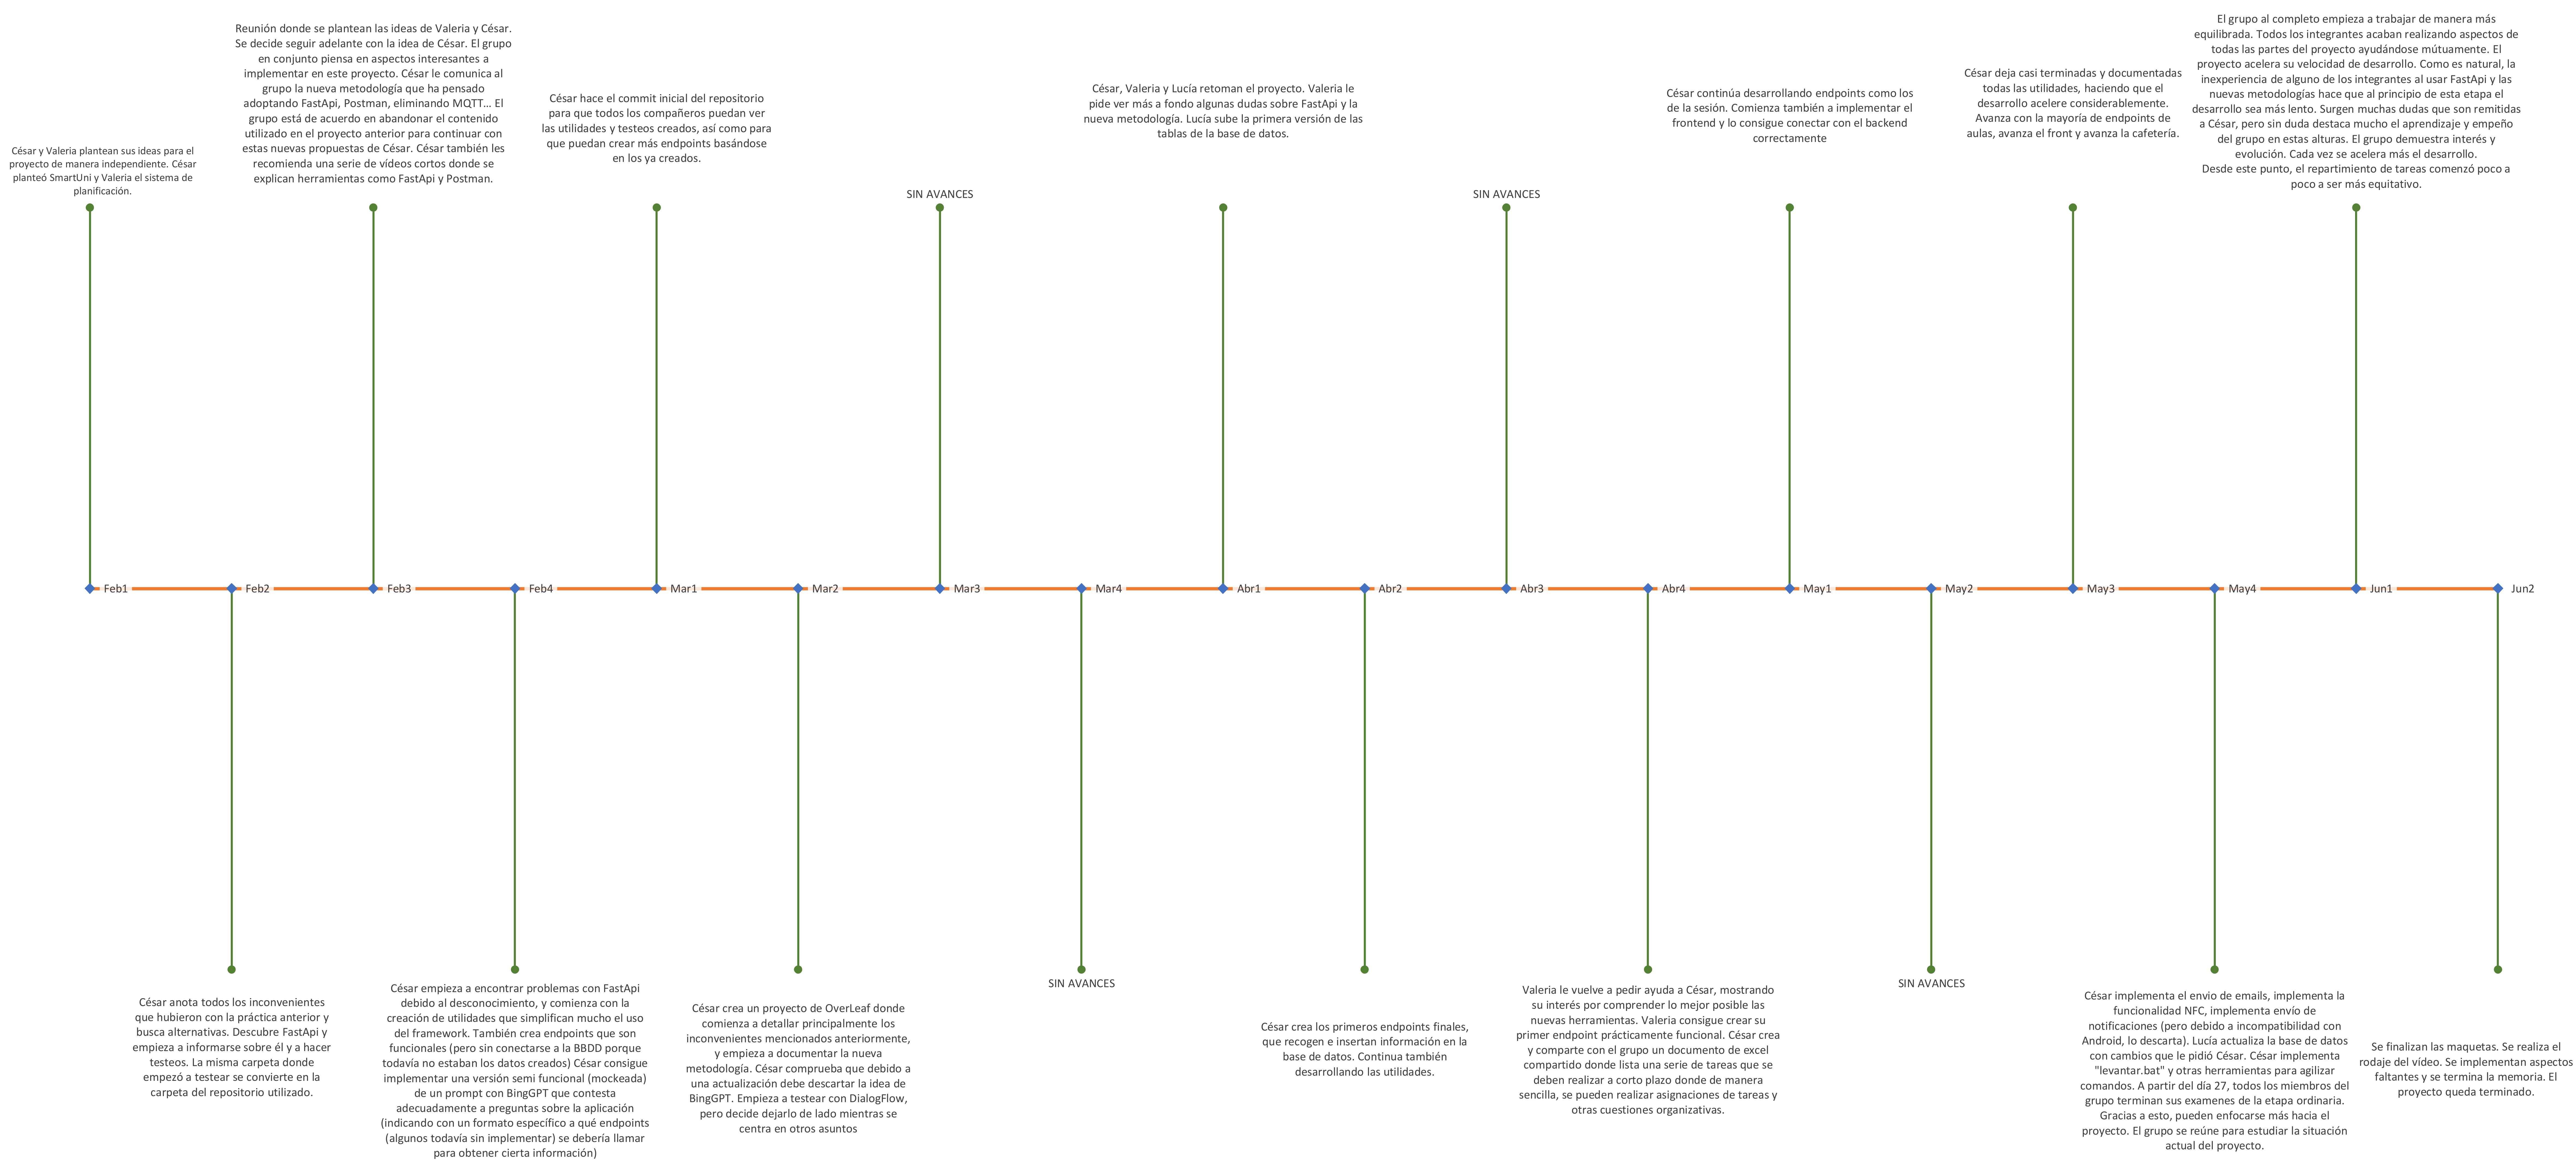
\includegraphics[width=1\linewidth]{imagenes//diagramas/linea de tiempo v2.png}
    \caption{Línea de tiempo del desarrollo de la práctica}
    \label{fig:enter-label}
\end{figure}
\end{landscape}
\newpage
\chapter{Conclusiones}
Indudablemente, el proceso de elaboración de este proyecto ha sido arduo. Un proyecto de esta magnitud siempre demanda un considerable esfuerzo por parte de todos los involucrados.\\

Durante el transcurso de esta práctica, hemos \textbf{adquirido} un amplio \textbf{conocimiento} y hemos demostrado nuestra capacidad para enfrentar desafíos de este nivel.\\

Nos sentimos \textbf{sumamente orgullosos} del resultado final de la práctica, a pesar de que nos hubiera gustado poder implementar funciones adicionales.\\

La utilización de \textit{FastApi} en el desarrollo nos ha permitido \textbf{acelerar} considerablemente el proceso, tal como se ha mencionado en secciones anteriores. Además, haber adoptado \textbf{metodologías más adecuadas}, como el uso de \textit{Postman} para realizar pruebas, ha dado \textbf{resultados notables}.\\

Nos entusiasmaría que en el futuro la Universidad de Alcalá \textbf{adoptara funcionalidades similares} a las que hemos propuesto en \textit{SmartUni}, lo que permitiría \textbf{modernizar y potenciar} la institución.


\newpage
\phantomsection
\addcontentsline{toc}{chapter}{10. Bibliografía}
\begin{thebibliography}{8}
    \bibitem{Repo} Repositorio del proyecto en GitHub, \url{https://github.com/CesarMartin2002/SmartUni}
    \bibitem{IoT} IoT en la educación, \url{https://www.fundacionbankinter.org/noticias/que-esta-aportando-internet-de-las-cosas-a-la-educacion/?_adin=02021864894}
    \bibitem{IoT en la ESO} IoT en las instituciones de educación superior, \url{https://www.researchgate.net/profile/Johan-Rueda-Rueda/publication/319914477_Internet_de_las_Cosas_en_las_Instituciones_de_Educacion_Superior/links/5b3e7dfb0f7e9b0df5f85931/Internet-de-las-Cosas-en-las-Instituciones-de-Educacion-Superior.pdf}
    \bibitem{IoT SW} Propuestas para el uso de IoT con herramientas de SW libre aplicado a la educación, \url{https://repository.unab.edu.co/bitstream/handle/20.500.12749/3410/2017_Tesis_Alvarez_Martinez_Adalberto.pdf?sequence=1}
    \bibitem{IoT educación} Aplicación de la tecnología del IoT en el ámbito educativo, \url{https://riunet.upv.es/bitstream/handle/10251/170674/Gimenez%20-%20Aplicacion%20de%20la%20tecnologia%20de%20Internet%20de%20las%20Cosas%20en%20el%20ambito%20educativo.pdf?sequence=1}
    \bibitem{IoT beneficios} IoT beneficios y claves en la educación,
    \url{https://cpvmicro.com/incorporando-iot-en-centros-educativos-aplicacion-y-beneficios/}
    \bibitem{ESP32}
    ESP32 enviar datos por POST y GET, \url{https://www.youtube.com/watch?v=uLkpILpQKuY&t=141s&ab_channel=IoTicos}
    \bibitem{Github ESP32}    Github: ESP32 POST \& REQUEST, \url{https://github.com/ioticos/esp32_esp8266_post_request/blob/master/src/main.cpp}
    \bibitem{Arduino Time} Arduino Time Library,     \url{https://playground.arduino.cc/Code/Time/}
    \bibitem{Video intro JavaScript} Vídeo de introducción a JavaScript, \url{https://youtu.be/2SetvwBV-SU}
    \bibitem{Web intro JavaScript} Web de introducción a JavaScript, \url{https://developer.mozilla.org/es/docs/Web/JavaScript}
    \bibitem{Web intro HTML} Web de introducción a HTML, \url{https://developer.mozilla.org/es/docs/Web/HTML}
    \bibitem{NFC} Interacción de NFC en Chrome por Android, \url{https://developer.chrome.com/articles/nfc/} 
    \bibitem{FastApi} FastApi con Python:  \url{https://www.youtube.com/watch?v=J0y2tjBz2Ao}
    \bibitem{API Bing Chat}Repositorio de la API de Bing Chat,  \url{https://github.com/acheong08/EdgeGPT}
\end{thebibliography}
\newpage

\begin{appendices}

\chapter{Manual de Usuario de la Aplicación Web}
A continuación se detallará el correcto modo de uso de la aplicación y los aparatos asociados a ella.
La aplicación es totalmente funcional en teléfonos Android e IOS, así como en Windows y macOS, salvo el escaneo de NFC, que solo es funcional en teléfonos Android.
Comenzaremos realizando una guía de la aplicación web y posteriormente una guía sobre el uso del aparato IoT.
\newpage
\section{Bienvenida}
Al abrir la página web accederá a la pagina de bienvenida donde tendrá la opción de iniciar sesión si ya posee un usuario y contraseña, o podrá registrarse en caso contrario.
\\En caso de querer iniciar sesión deberá introducir el correo electrónico asociado a su cuenta en el campo de texto marcado como (1) y su contraseña en el campo (2), una vez rellenados esos campos con la información de su cuenta podrá pulsar el botón de iniciar sesión (3) y se le redirigirá a la página de menú, A.3. 
\\En caso de que no posea una cuenta, siempre podrá crearse una pulsando en registrarte (4), lo cual le redirigirá a la página de registro, A.2.\\
\begin{figure}[H]
    \centering
    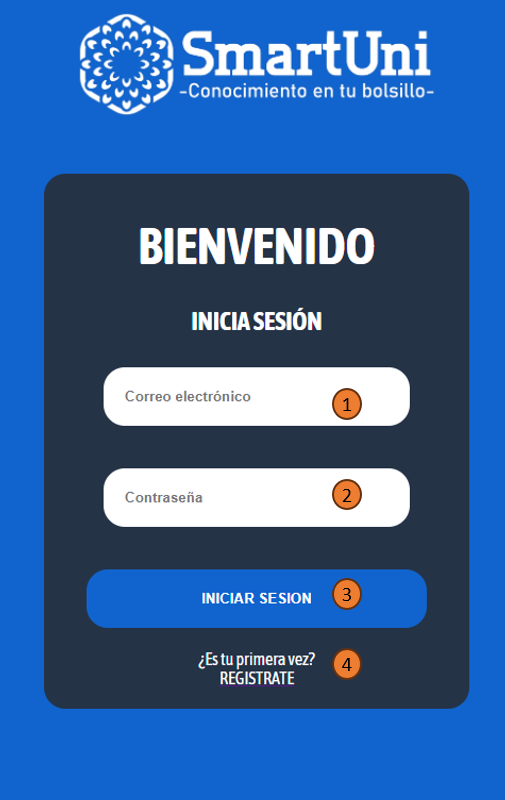
\includegraphics[scale = 0.7]{imagenes//manual_de_usuario/1.png}
    \caption{Inicio}
    \label{fig:Figura3.4.3}
\end{figure}
\newpage
\section{Registro}
Una vez pulsado registrarse en la página de bienvenida será redirigido aquí, donde rellenando los distintos campos se podrá crear su cuenta para disfrutar de los servicios de la aplicación.
\\\\Para crear su cuenta deberá rellenar todos los campos con la información de la cuenta a crear. En el campo de correo electrónico (1) deberá insertar el correo electrónico al que desea vincular su cuenta, seguido de esto deberá escribir su contraseña en el campo (2) y (3) para verificar que no se ha equivocado a la hora de escribir la contraseña, una vez rellenados esos datos podrá pulsar el botón de registrarse (4) y se le redirigirá al menú A.3, en caso de haber entrado a esta página por error o si ya tiene una cuenta podrá pulsar el botón de iniciar sesión (5), lo que le devolverá a la pagina de bienvenida A.1.\\
\begin{figure}[H]
    \centering
    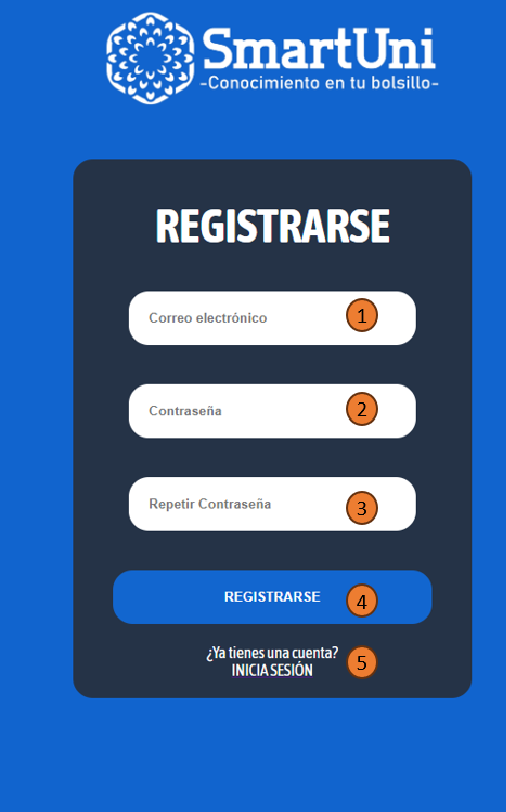
\includegraphics[scale = 0.7]{imagenes//manual_de_usuario/3.png}
    \caption{Registrarse}
    \label{fig:Figura3.4.3}
\end{figure}
\newpage
\section{Menú}
El menú muestra las diferentes secciones del programa a las que puede acceder, el botón (1) le redirigirá al listado de las aulas,A.4, donde podrá ver las diferentes aulas de la Escuela Politécnica Superior y qué se imparte en ellas; el botón (2) le redirigirá a su taquilla, A.8, si posee una o al listado de taquillas, A.6, donde podrá reservar una para uso personal; el botón (3) le llevará a la sección de cafetería, A.9, donde podrá realizar un pedido de manera remota para poder recogerlo y disfrutar de la comida de la cafetería. Si quiere salir de la aplicación podrá pulsar el botón cerrar sesión (4).\\
\begin{figure}[H]
    \centering
    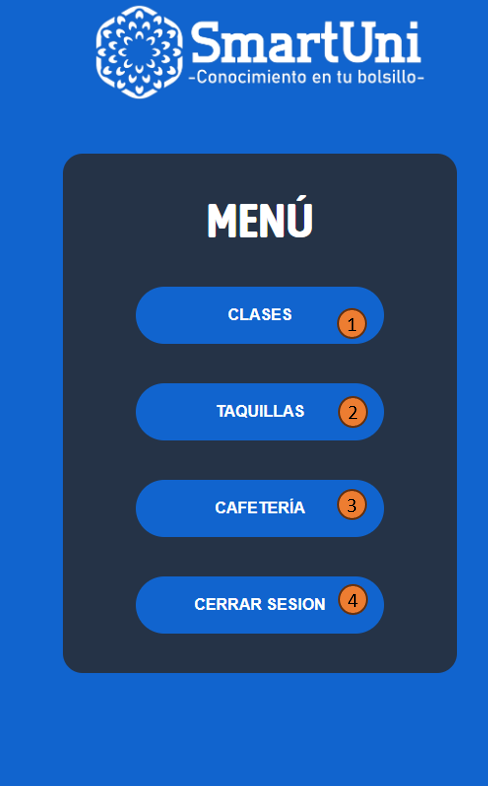
\includegraphics[scale = 0.7]{imagenes//manual_de_usuario/2.png}
    \caption{Menú}
    \label{fig:Figura3.4.3}
\end{figure}
\newpage
\section{Listado de aulas}
Esta página muestra un listado dentro del Box(2) de todas las aulas de las que se dispone información, para ver en detalle la información del aula deberá pulsar el botón del aula que desee(3). En caso de querer volver al menú, podrá pulsar la imagen de SmartUni de la parte superior de la pantalla(1).\\
\begin{figure}[H]
    \centering
    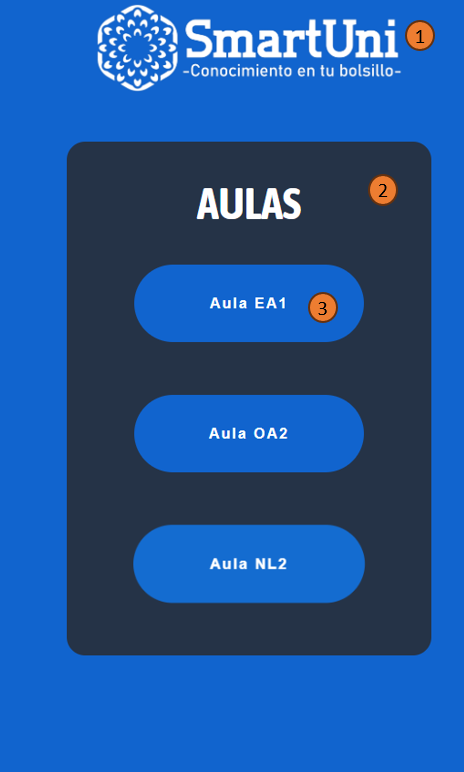
\includegraphics[scale = 0.7]{imagenes//manual_de_usuario/4.png}
    \caption{Listado de aulas}
    \label{fig:Figura3.4.3}
\end{figure}
\newpage
\section{Detalle de un aula}
En esta página se detallará la información disponible sobre el aula, como puede ser la temperatura o las asignaturas que se imparten en ella junto a sus horarios. En caso de querer volver al menú, podrá pulsar la imagen de SmartUni de la parte superior de la pantalla(1).\\
\begin{figure}[H]
    \centering
    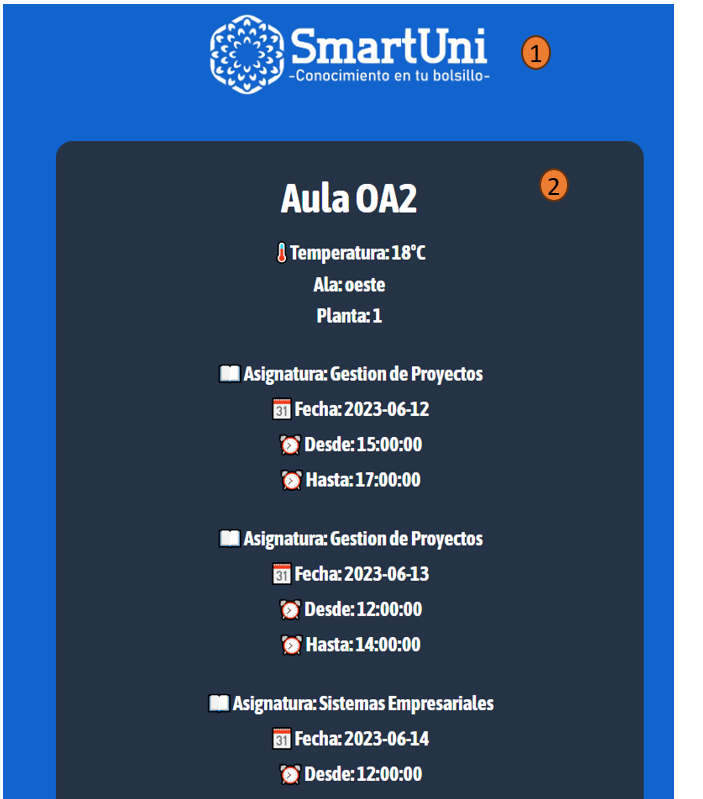
\includegraphics[scale = 0.7]{imagenes//manual_de_usuario/5.png}
    \caption{Detalle de un aula}
    \label{fig:Figura3.4.3}
\end{figure}
\newpage
\section{Listado de taquillas}
Esta página muestra un listado dentro del Box(2) de todas las taquillas disponibles, para ver en detalle la información de la taquilla deberá pulsar el botón de la taquilla que desee(3). En caso de querer volver al menú, podrá pulsar la imagen de SmartUni de la parte superior de la pantalla(1).\\
\begin{figure}[H]
    \centering
    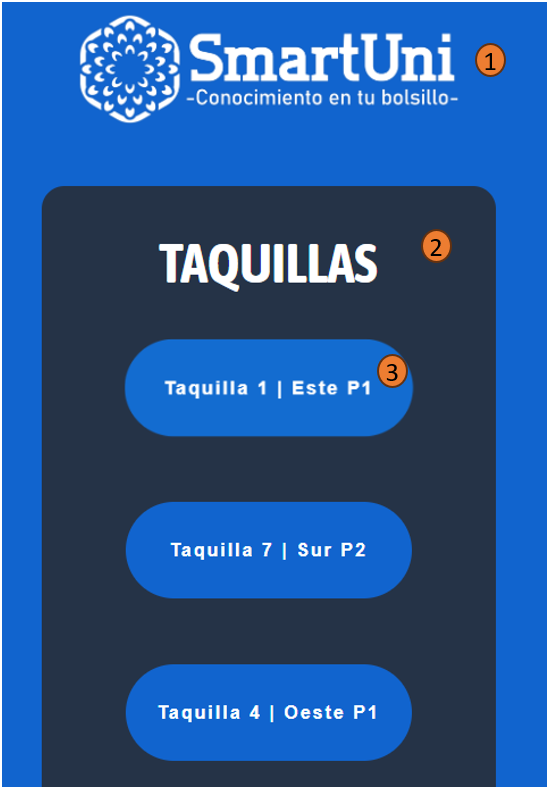
\includegraphics[scale = 0.7]{imagenes//manual_de_usuario/6.png}
    \caption{Listado de taquillas}
    \label{fig:enter-label}
\end{figure}
\newpage
\section{Reserva de Taquilla}
En esta página se ve la información disponible de la taquilla(2), también se puede ver el botón de solicitar taquilla(3), que al pulsarlo le dirigirá a A.7 y vinculará la taquilla a su usuario. En caso de querer volver al menú, podrá pulsar la imagen de \textit{SmartUni} de la parte superior de la pantalla(1).\\
\begin{figure}[H]
    \centering
    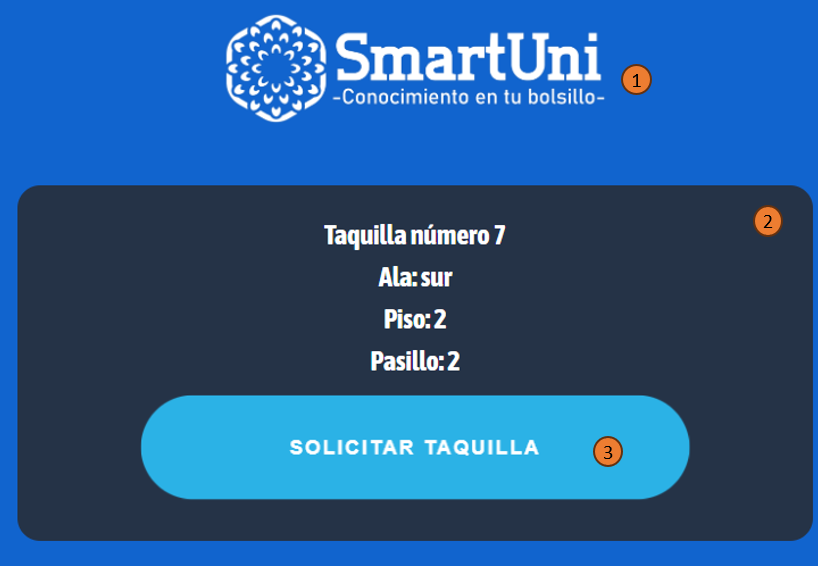
\includegraphics[scale = 0.7]{imagenes//manual_de_usuario/8.png}
    \caption{Reservar una taquilla}
    \label{fig:Figura3.4.3}
\end{figure}
\newpage
\section{Taquilla reservada}
Una vez reservada la taquilla podremos acceder a esta página en la que se mostrará la información de la taquilla incluyendo la contraseña con la que se podrá abrir la taquilla pertinente, se dispone del botón de cancelar taquilla(3), que desvinculará la cuenta de la taquilla. En caso de querer volver al menú, podrá pulsar la imagen de SmartUni de la parte superior de la pantalla(1).\\
\begin{figure}[H]
    \centering
    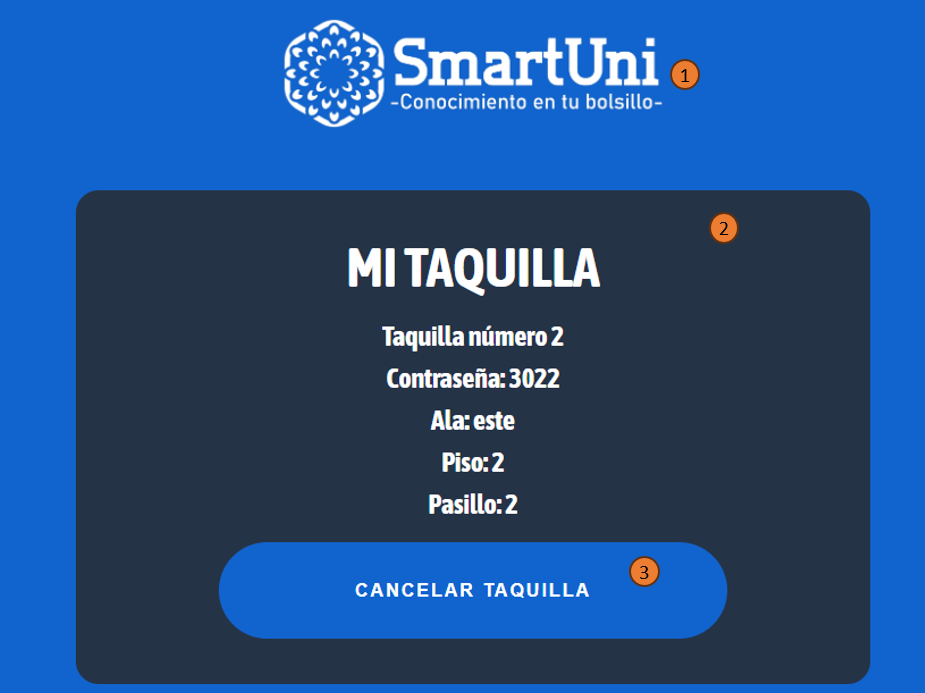
\includegraphics[scale = 0.7]{imagenes//manual_de_usuario/7.png}
    \caption{Detalle de una taquilla}
    \label{fig:enter-label}
\end{figure}
\newpage
\section{Inicio de cafetería}
Esta pagina representa el inicio de la cafetería, en ella se puede realizar un pedido(2), pulsando este botón accederá a A.10. o acceder a los pedidos que ya ha realizado(3), que le redirigirá a A.11. En caso de querer volver al menú, podrá pulsar la imagen de SmartUni de la parte superior de la pantalla(1).\\
\begin{figure}[H]
    \centering
    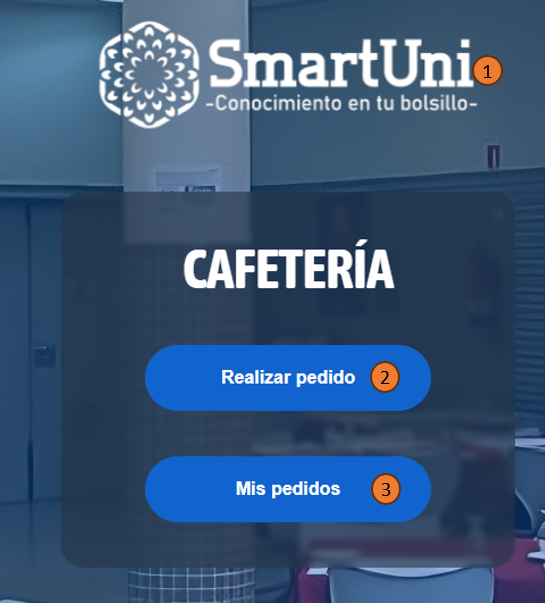
\includegraphics[scale = 0.7]{imagenes//manual_de_usuario/9.png}
    \caption{Inicio de la cafetería}
    \label{fig:enter-label}
\end{figure}
\newpage
\section{Realizar Pedido}
En esta página podrá realizar su pedido de la cafetería, en ella dispone de información como recomendaciones generales y personalizadas(2). 
\\\\También dispondrá de un buscador en el que podrá filtrar los productos por su nombre(3). Para seleccionar sus productos dispone de un listado de botones(5) con los cuales podrá rellenar su pedido. Cada producto esta relacionado a 3 botones, el principal que es el central(7) mostrará la información del producto junto con una foto de él, el botón de +(8), que añadirá una unidad del producto seleccionado a la cesta de compra, y el botón -(6), que quitará una unidad del producto seleccionado a la cesta de compra. \\\\Una vez seleccionados todos los productos, se confirmará el pedido pulsando en el botón Confirmar(4). En caso de querer volver al menú, podrá pulsar la imagen de SmartUni de la parte superior de la pantalla(1).\\
\begin{figure}[H]
    \centering
    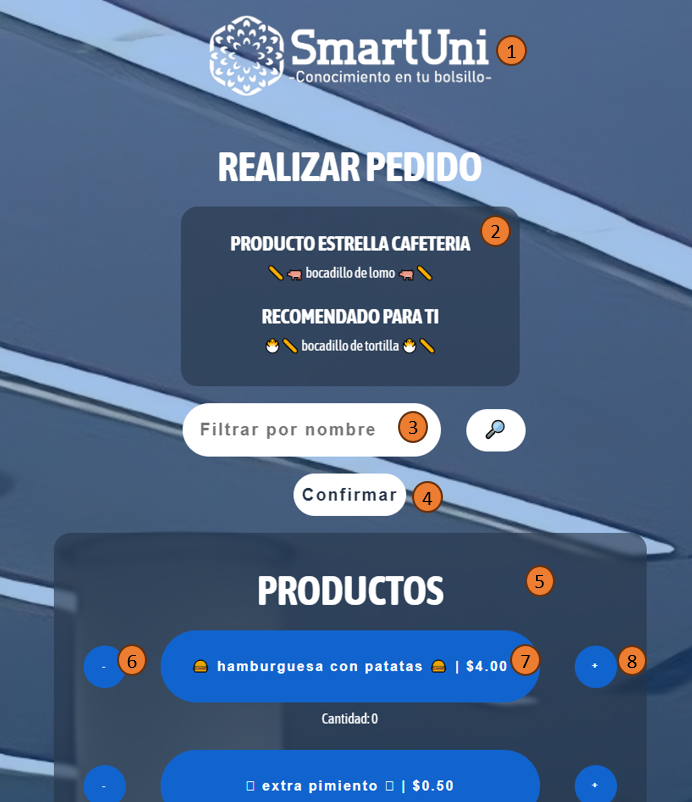
\includegraphics[scale = 0.65]{imagenes//manual_de_usuario/10.png}
    \caption{Realizar pedido}
    \label{fig:enter-label}
\end{figure}
\newpage
\section{Seleccionar pedido}
En esta pagina podrá ver los diferentes pedidos que haya realizado(2), al pulsar en su pedido(3), se le redirigirá a A.12. Los pedidos marcados en rojo son pedidos ya finalizados o cancelados. En caso de querer volver al menú, podrá pulsar la imagen de SmartUni de la parte superior de la pantalla(1).\\
\begin{figure}[H]
    \centering
    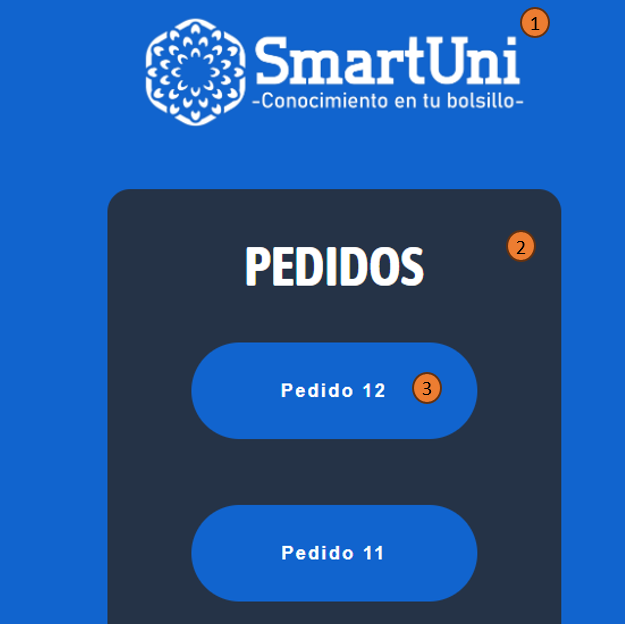
\includegraphics[scale = 0.7]{imagenes//manual_de_usuario/12.png}
    \caption{Seleccionar pedido}
    \label{fig:enter-label}
\end{figure}
\newpage
\section{Información de un pedido}
Esta pagina muestra la información del pedido seleccionado(2), en ella además se podrá escanear el NFC(3) correspondiente a su pedido, la información sobre este NFC se dispondrá en el momento en que se asocie el pedido a una bandeja. Así como poder simularlo(4), este botón simulara la conexión con el NFC de manera ficticia. Además se puede avanzar el estado de su pedido, lo cual esta implementado solo para prueba de pedidos y es un botón experimental. En caso de querer volver al menú, podrá pulsar la imagen de SmartUni de la parte superior de la pantalla(1).
\\
\begin{figure}[H]
    \centering
    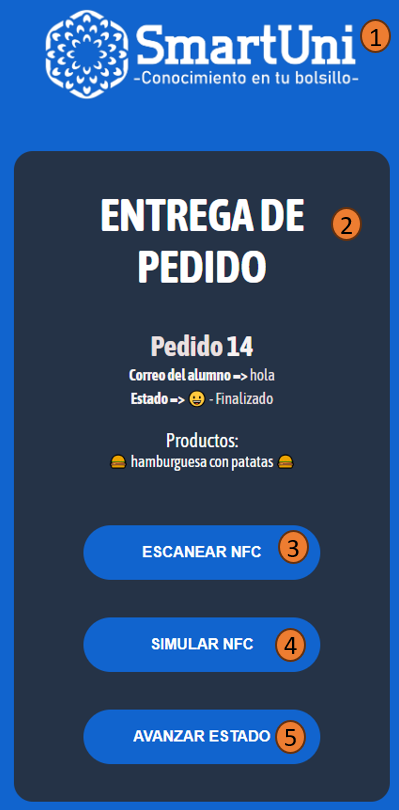
\includegraphics[scale = 0.7]{imagenes//manual_de_usuario/11.png}
    \caption{Información de un pedido}
    \label{fig:enter-label}
\end{figure}
\newpage
\section{Uso de la Taquilla}
Una vez se ha reservado una taquilla, esta tendrá asociada una única contraseña con la que se podrá abrir la taquilla tecleando dicha contraseña en el teclado situado en la parte frontal de la taquilla. Podrá saber si ha introducido correctamente la contraseña si al introducirla se enciende el led 2 veces y a su vez suenan dos señales del buzzer actuador, en caso de error serán 3 veces. Una vez abierta la taquilla podrá depositar sus pertenencias en ella. Para cerrar la taquilla cierre la puerta de la taquilla de forma que empiece a oír un pitido, este se repetirá 5 veces para indicar que la taquilla esta cerrándose. Cabe aclarar que es imperativo no cubrir el orificio situado a la izquierda del marco de la taquilla ya que en el caso de cubrirlo la taquilla no podrá realizar el cierre de esta. El mal uso de este equipo puede conllevar al veto de los servicios de SmartUni.
\section{Recogida de pedido}
En el momento que haya realizado un pedido, espere a que este se asocie a un NFC, cuando este proceso haya terminado y el pedido este listo para recoger, simplemente pulse el botón de escanear NFC y acerque su dispositivo móvil a la bandeja con el NFC indicado en su dispositivo. Podrá reconocer las bandejas ya que en ellas esta indicado el número del NFC que contiene. Es preciso mencionar que este sistema no esta disponible para dispositivos IOS ni ordenadores portátiles o de sobremesa.

\newpage
\chapter{Simulación de datos}

En el proyecto, se han generado datos tanto físicos como virtuales. Por ejemplo, además de la taquilla física representada por el Arduino, existen varias taquillas en el sistema. Lo mismo ocurre con las aulas, donde se han implementado diversas aulas en el sistema, aunque solo se haya relacionado físicamente una de ellas con el Arduino.\\

De hecho, es sencillo configurar el Arduino para simular diferentes aulas o taquillas, simplemente modificando el identificador asociado en el código del Arduino.\\

Por otro lado, la disponibilidad de todos estos datos nos permite realizar simulaciones de uso de la plataforma. A través del archivo "simulaciones.py", se pueden realizar llamadas a varios métodos de la API. Estos métodos permiten simular reservas y cancelaciones de taquillas, así como solicitudes de pedidos a la cafetería, entre otros.\\

Es importante destacar que este archivo debe ejecutarse por separado, independientemente de si el servidor está activo o no. Al ejecutarlo, se seleccionará de manera aleatoria un identificador de alumno, así como una llamada a ejecutar en la API. Los resultados de estas simulaciones se mostrarán en tiempo real en la terminal.

\newpage
\chapter{Hojas de características de los componentes}
A continuación, se adjuntarán las distintas hojas de los componentes empleados en el prototipado:
\begin{itemize}
    \item \textbf{Sensor de ultrasonidos}: \url{https://cdn.sparkfun.com/datasheets/Sensors/Proximity/HCSR04.pdf}
    
    \item \textbf{Sensor de humedad y temperatura DHT11}: \url{https://datasheet.octopart.com/386-Adafruit-Industries-datasheet-81453130.pdf}
    
    \item \textbf{Servomotor sg90}: \url{http://www.ee.ic.ac.uk/pcheung/teaching/DE1_EE/stores/sg90_datasheet.pdf}
    
    \item \textbf{Buzzer}: \url{https://www.farnell.com/datasheets/2171929.pdf}
    
    \item \textbf{Led rojo}: \url{https://www.farnell.com/datasheets/1498852.pdf}
    
    \item \textbf{Keypad}: \url{http://www.electronicoscaldas.com/datasheet/Teclado-membrana-matricial-4x4.pdf}
    
    \item \textbf{ESP32}: \url{http://www.edu.xunta.gal/centros/ieslaxeiro/system/files/ESP-32%20Dev%20Kit%20C%20V2_EN.pdf}
    
    \item \textbf{NFC}: \url{https://www.nxp.com/docs/en/data-sheet/NTAG213_215_216.pdf}
\end{itemize}

\newpage
\end{appendices}
\end{document}
